%%%%%%%%%%%%%%%%%%%%%%%%%%
%%% ENVIRONMENT SETUP  %%%
%%%%%%%%%%%%%%%%%%%%%%%%%%

\documentclass[12pt, twoside, openright]{book}
%%% DEPENDENCIES ETC
\usepackage[utf8]{inputenc}
%importing pdfs keeping track of page number
\usepackage{pdfpages}
%page format (margins etc
\usepackage[a4paper, width=150mm, top=25mm,bottom=25mm, bindingoffset=6mm]{geometry}
% disable automatical indentation
\setlength{\parindent}{0pt} 
%fancy headers and footers
\usepackage{lastpage}
\usepackage{fancyhdr}
\pagestyle{fancy}
%mathsymbols
\usepackage{amssymb}
%images
\usepackage{graphicx} 
\graphicspath{{misc/}}
\usepackage[font={footnotesize, it}]{caption}

\usepackage{subcaption}

% tables https://tex.stackexchange.com/questions/75793/tabular-input-by-columns-i-e-transpose-a-table
\usepackage{booktabs,array}
\def\Midrule{\midrule[\heavyrulewidth]}
\newcount\rowc

\makeatletter
\def\ttabular{%
  \hbox\bgroup
  \let\\\cr
  \def\rulea{\ifnum\rowc=\@ne \hrule height 1.3pt \fi}
  \def\ruleb{
    \ifnum\rowc=1\hrule height 1.3pt \else
    \ifnum\rowc=6\hrule height \heavyrulewidth 
    \else \hrule height \lightrulewidth\fi\fi}
  \valign\bgroup
  \global\rowc\@ne
  \rulea
  \hbox to 10em{\strut \hfill##\hfill}%
  \ruleb
  &&%
  \global\advance\rowc\@ne
  \hbox to 10em{\strut\hfill##\hfill}%
  \ruleb
  \cr}
\def\endttabular{%
  \crcr\egroup\egroup}

% python color code
\usepackage{listings}
% \usepackage{minted}

% mindmaps
\usepackage{tikz}
\usetikzlibrary{trees}

% color box for math formulas
\usepackage[most]{tcolorbox}

% thick 1 function: doublestroke package
\usepackage{dsfont}
\usepackage{bbm}

% rotate figures
\usepackage[figuresleft]{rotating}

\fancyhead[LO,LE]{\fontsize{10}{12}\selectfont\leftmark}  % \nouppercase\leftmark
\fancyhead[RO,RE]{\fontsize{9}{12}\selectfont\nouppercase\rightmark}

% lorem ipsum dummy text generator
\usepackage{lipsum}

% for links
\usepackage{url}
% for math symbols etc
\usepackage{mathtools}

% bibliography manager
\usepackage[backend=biber]{biblatex}
\addbibresource{misc/references.bib}



%%%%%%%%%%%%%%%%%%%%%%%%%%
%%% GLOBAL DEFINITIONS %%%
%%%%%%%%%%%%%%%%%%%%%%%%%%

%%% CHANGE BULLETS FOR LISTING
%%% original ones: $\bullet$, $\cdot$, $\diamond$, $\ast$
\renewcommand{\labelitemi}{---}
\renewcommand{\labelitemii}{$\circ$}
\renewcommand{\labelitemiii}{$\ast$}
\renewcommand{\labelitemiv}{$\cdot$}



%%%%%%%%%%%%%%%%%%%%%%%%%%
%%% START DOCUMENT     %%%
%%%%%%%%%%%%%%%%%%%%%%%%%%
\begin{document}


\includepdf{misc/cover.pdf}
%blank page
\newpage
\thispagestyle{empty}
\mbox{}

\frontmatter

\chapter*{Declaration of Authorship/\\Eidesstattliche Erkl\"arung}
\addcontentsline{toc}{chapter}{Declaration of Authorship/Eidesstattliche Erkl\"arung}
{\Large \textbf{English}}\\
``I do solemnly declare that I have written the presented research thesis by myself and without help from any sources other than that specified, respecting the {\it policy regarding good scientific practice}\cite{goethepolicy}.\\

Where I have used thoughts from external sources, directly or indirectly, published or unpublished, this is always clearly attributed.\\

I certify that this research thesis or any part of it has not been previously submitted for a degree or any other qualification at this University or any other institution in Germany or abroad.''\\[6mm]


{\Large \textbf{Deutsch}}\\
``Hiermit erkl\"are ich, dass ich die Bachelorarbeit selbst\"andig und ohne Benutzung anderer als der angegebenen Quellen und Hilfsmittel verfasst habe.\\

Alle Stellen, die wörtlich oder sinngemäß aus veröffentlichten oder noch nicht veröffentlichten Quellen entnommen sind, sind als solche kenntlich gemacht.\\

Diese Arbeit ist in gleicher oder ähnlicher Form noch bei keiner anderen Prüfungsbehörde eingereicht worden.''\\[6mm]



{\Large \textbf{Signature/Unterschrift}}\\

In Frankfurt am Main, \underline{\hspace{3.5cm}}, 2017\\[2.3cm]
(Signature/Unterschrift)\\%/Datum und Unterschrift:\\

Name/Name: \textbf{Andr\'es Fern\'andez Rodr\'iguez}\\
Matriculation No./Matrikelnummer: \textbf{5692442}\\

%% Examination No.: \textbf{}\\
%% Submission Date:  \textbf{}\\

%blank page
\newpage
\thispagestyle{empty}
\mbox{}

\chapter*{Abstract}
\addcontentsline{toc}{chapter}{Summary}
Among the variety of topics within music classification using machine learning, automatic classification of carnatic r\=agas is an interesting and suitable task for a bachelor's thesis, because the task is relatively well defined in its both musical and technical dimensions, and its intrinsic difficulty involves the study of a variety of recent approaches.\\

The state of the art for such task shows a clear dominance of the domain-specific solutions, with no successful end-to-end approach reported. This poses the question, whether such an end-to-end approach could be possible for the current tools and data avaliable.\\

In order to explore that question, the experiments conducted in the context of the present thesis applied several convolutional neural networks to perform end-to-end supervised learning on the CompMusic carnatic corpus, refraining from applying such domain-specific solutions.\\

The results of the experiments were that the different tested setups were unable to learn any relevant features for this task, possibly due to the inefficience of the chosen representation for the given amount of data.

%blank page
\newpage 
\thispagestyle{empty}
\mbox{}

\chapter*{Acknowledgements}
\addcontentsline{toc}{chapter}{Foreword and Acknowledgements}
I want to thank and dedicate this work to my beloved family for their constant support. Also to Professor Ramesh, Tobi, Sreenivas and especially to Martin for their careful supervision and helpful insights.\\

Last but not least, to Professor Serra's team at the Universitat Pompeu Fabra in Barcelona, for kindly sharing their data and work.\\

Thank you all.

%blank page
\newpage 
\thispagestyle{empty}
\mbox{}

\tableofcontents


% LIST OF FIGURES
\cleardoublepage
% \phantomsection
\addcontentsline{toc}{chapter}{\listfigurename}
\listoffigures
\addcontentsline{toc}{chapter}{\listtablename}
\listoftables

\mainmatter

\chapter{Summary} \label{problem-def}
The present thesis explores the question, whether an end-to-end approach could be successful in automatically learning and performing r\=aga classification, in comparison to existent domain-specific approaches.\\

For that, it starts by a description of the used dataset and the motivations behind its curation in chapter \ref{about-ds}, followed by a brief overview on carnatic music in chapter \ref{about-car}, necessary to achieve a better understanding of the related work and to provide some basis to help the interpretation of the experimental results.\\

Chapter \ref{context} reports the domain-specific approaches that conform the state of the art in r\=aga classification, as well as some recent and successful end-to-end approaches in the related field of Music Genre Recognition (MGR), which serve in this thesis as reference to apply to the r\=aga classification problem.\\

Chapter \ref{about-ml} follows providing a technical basis useful to understand the implementation of the concepts explained in chapter \ref{implementation}.\\

The final chapters \ref{experiments} and \label{conclusion} report the experiments done, as well as the line of thought behind them including motivations, interpretations and possible follow-ups.


\chapter{About the Dataset} \label{about-ds}
This chapter describes briefly the origins and motivations that lead to the collection and curation of the data used in this thesis, as well as some of its main features.


\section{The CompMusic Project}\label{compmsc}

The mp3 files and labels comprising the carnatic corpus that was used in this thesis were gathered as part of the {\it CompMusic: Computational Models for the discovery of the world's music} project, promoted by Professor Xavier Serra at the Universitat Pompeu Fabra (Barcelona) since 2011 and funded by the European Research Council. As described by Professor Serra himself\cite{serra-comp14}, ``The focus of the project lies on computational approaches to describe music recordings by emphasising the use of domain knowledge of particular music traditions, focusing on five music cultures: Arab-Andalusian (Maghreb), Beijing Opera (China), Turkish-makam (Turkey), Hindustani (North-India) and Carnatic (South-India)''. This can be encompassed within the scientific field of Music Information Research (MIR), which ``primarily addresses topics involved in the understanding and modeling of music using information processing methodologies. In particular, it aims to advance our knowledge in representing, understanding, describing, retrieving, archiving and organizing music related data''\cite[p.3]{gulati}.\\

Specifically, CompMusic aims to help overcoming the information bias towards western music present in the MIR field, in order to achieve a broader and more profound understanding of different culture-specific musical phenomena, as well as develope domain-specific research methodologies more appropiate to solve them. Part of the underlying thesis is that ``addressing the research problems in the context of diverse music cultures will not only help in advancing the knowledge in the specific cultures, but also expand the scope of the state of the art in MIR''\cite[p.4]{gulati}. Further quoting, ``Among ethnomusicologists there is a wide consensus that all musics are not alike, and that the approaches used to understand Western musics are not appropriate for other types of musics.''\cite{serra-comp14}. A further and very detailled explanation on the motivations and implications of the project can be found in \cite{serra-comp11} and \cite{serra-comp14}.\\

The creation and curation of the diferent corpora in the context of the CompMusic project responds to a double motivation: it allows the reproducibility of the experiments, and also serves as basis for any data-driven approach that may also be undertaken. For that sake, the CompMusic project has developed the Dunya platform, ``a tool for navigating through music collections which also acts as the central permanent online repository to store the metadata, audio, annotations and research results. Dunya is open source and provides an API for accessing these data''\cite{indian-corpora}.\\

Prof. Serra's research group kindly granted us access to the platform's contents via its open API (\url{https://github.com/MTG/dunya}), and, for the carnatic corpus, we were able to download a total of 2455 labeled recordings as high-quality mp3 files of different lengths. The labels comprise ten different domains: \texttt{r\=aga}, \texttt{form}, \texttt{title}, \texttt{work}, \texttt{album\_artists}, \texttt{t\=a\d{l}a}, \texttt{length}, \texttt{artists}, \texttt{mbid} and \texttt{concert}. The histograms of total length and number of recordings per class can be found in appendix \ref{ds-stats}, for all domains except \texttt{length}, \texttt{title} and \texttt{work} (since they would have one class per sample and such histograms wouldn't be meaningful). Bear in mind that, in some domains, a single recording may appear in several classes (for instance, an ensemble has always several \texttt{album\_artists}), and, for some recordings, several domains may remain unlabeled hence not appearing in all the histograms. Therefore, the overall distribution is different for each domain. The 2014 article cited in \cite{indian-corpora} contains some further statistics, but the corpus has changed considerably since then, as it can be seen in the data presented here (for example, now it has over 500 more recordings, but 25 less r\=agas). In any case, the article contains also further useful information about the agents involved in the compilation and labelling process of all CompMusic's corpora, which may be interesting for curation purposes but outside of the scope of this thesis.\\

For a more detailled description of the dataset's musical contents, see chapter \ref{about-car}.


\section{The R\=aga Recognition Dataset (\(RRD_{CMD}\))} \label{rrd_cmd}

A relevant subset of the carnatic corpus in the context of this thesis is the (\(RRD_{CMD}\)) dataset, introduced by Gulati et al. in 2016 (see \cite[p.84]{gulati}). As a part of the CompMusic project, \(RRD_{CMD}\) was selected and curated to provide a sizable, fixed subset that would fullfill the above mentioned criteria of purpose, coverage, completeness, quality and reusability (as stated in \cite[pages 7, 10 and 83]{gulati}: see chapter \ref{about-car} for more details on the different r\=agas and their musical aspects).  Its main features are pictured in Figures \ref{fig:rrd-overall} and \ref{fig:rrd-ragasvaras}.\\

As explained in \cite[p.61]{gulati}, this test dataset responds to the idea of a static collection (as opposed to a research corpus which can evolve over time) that allows benchmarking and reproducibility of the research results. More specifically, it notes that it ``should not be confused with the training and testing split of a dataset, which are the terms used in the context of a cross validation experimental setup''. For an explanation about this ``cross validation experimental setup'', see \cite[p.121]{goodfellow}.\\

The dataset features are open and accessible in GitHub: \url{https://github.com/sankalpg/MelodicAnalysisDatasets/tree/master/RagaDataset/Carnatic}.\\
From its 480 listed recordings, only 439 were present in the Dunya platform at the moment of downloading. This remaining subset, noted as \(RRD^*\) from now on, is therefore smaller, but still similarly distributed, as it can be seen in Table \ref{fig:rrd-stats}.

\begin{figure}[h]
  \centering
  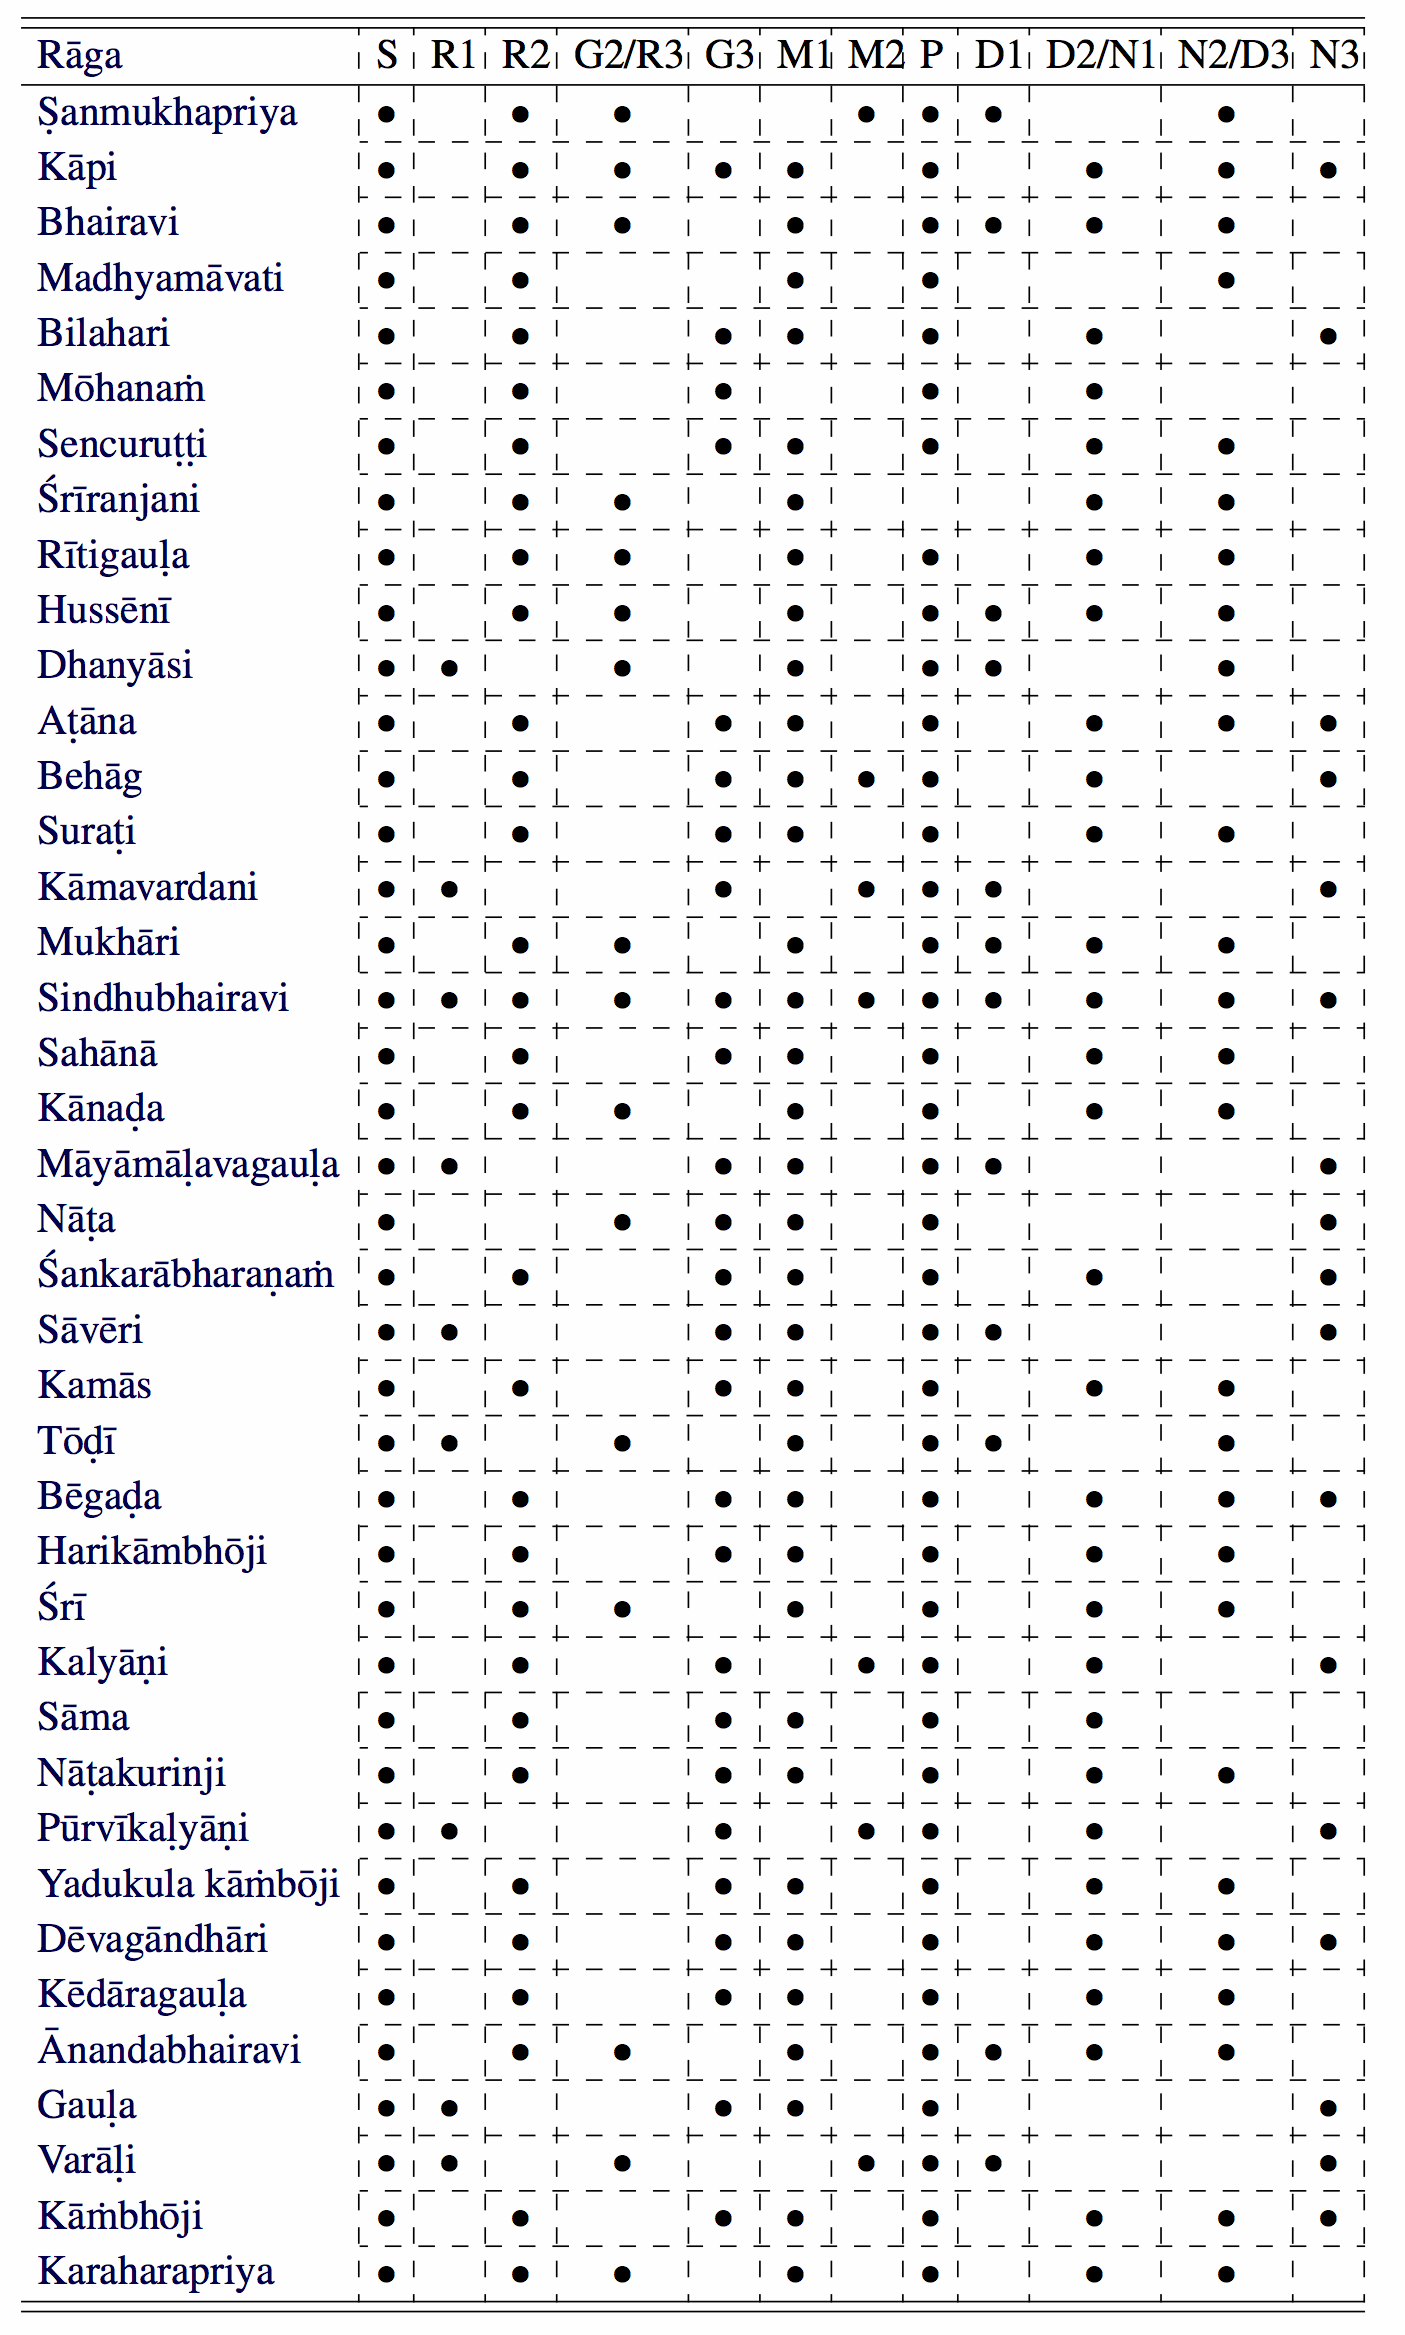
\includegraphics[scale=0.28]{raga_svaras.png}
  \caption{List of the r\=agas in (\(RRD_{CMD}\)) along with their constituent set of svaras. The contents of this table are verified by Vignesh Ishwar, a professional vocalist of carnatic music (from \cite[p.244]{gulati}. See chapter \ref{about-car} of the present thesis for a more detailled description of the r\=agas).}
  \label{fig:rrd-ragasvaras}
\end{figure}

\begin{figure}[h]
  \centering
  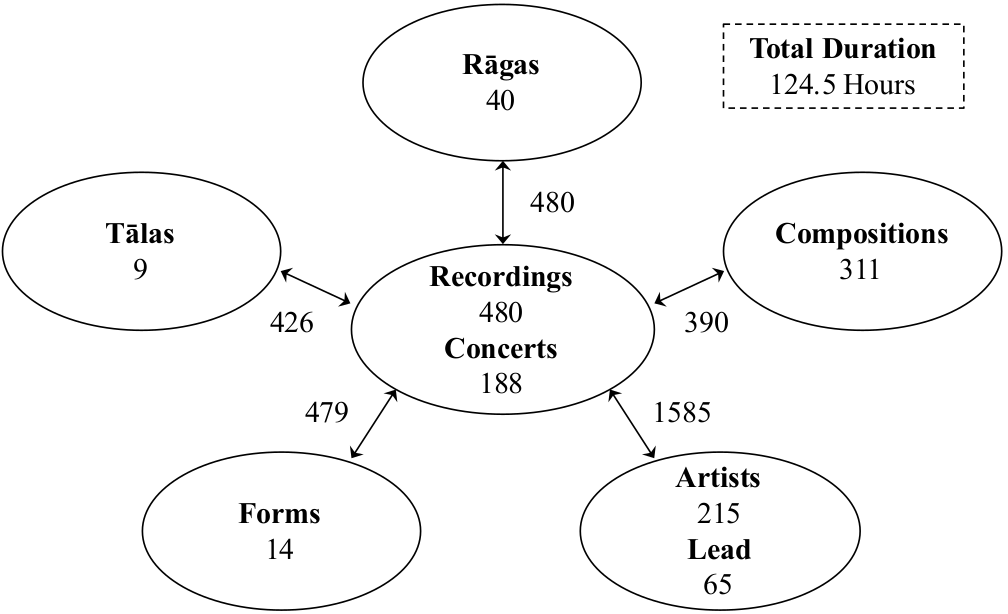
\includegraphics[scale=0.4]{rrd_gulati.png}
  \caption{Details of the rāga recognition dataset (\(RRD_{CMD}\)) comprising Carnatic music recordings in terms of the number of different musical entities and relationships between them. (from \cite[p.85]{gulati}).}
  \label{fig:rrd-overall}
\end{figure}


\chapter{About Carnatic Music} \label{about-car}
Carnatic and hindustani are two musical traditions in the indian subcontinent that are referred to as Indian Art Music (IAM), and whose common roots can be traced back to around 1000 BC\cite[p.15]{gulati}. They have many elements in common, but also notable differences. This chapter intends to provide a brief overview on carnatic music, in order to support a good understanding of the related work in chapter \ref{context}, and provide some basis to help the interpretation of the results of chapter \ref{conclusion}.\\

For that, it will cover first the aesthetical aspects that reflect the idiosyncrasy of its cultural context. This will help to understand the main features of the carnatic concert, the quintessential manifestation this music takes place in, described in the middle section. The last section of this chapter about carnatic music will describe the main elements of the proper musical discourse that are relevant in the context of the present thesis.


\section{Aesthetical Aspects}

Among the many artists present in the carnatic music corpus presented in \ref{about-ds}, Thodur Madabusi Krishna is present with six recorded concerts. Apart from playing carnatic music, he also captured his view of it in a book\cite{krishna}, in which he gives some insights that cana be helpful to understand the components and goals of carnatic music as a cultural phenomenon: ``Karnatik music is a most interesting form in its function within the social fabric and its own evolution. What makes it so is that its function is based on the musical aspects that constitute its existence. These are: raga, tala, composition and improvisation. The function of the musician is to express the various melodic and rhythmic aspects of the music with a complete understanding of its aesthetics and grammar. The musician is neither conveying a social message nor helping interpret a certain theatrical act or delivering a religious experience''\cite[p.30]{krishna}.\\

In fact, even when the music is featuring the human voice, he warns that, apart from the emotional and ideological dimensions that may take part in the artist's creative process, ``when presented in a Karnatik music concert, the focus is on the beauty of the language, its sounds, syllables and their interactions with the raga and tala'' because ``within the context of art music, there is no reason for the creation of music other than the music itself''\cite[p.33]{krishna}. And to clarify this focus even more, he finishes his thoughts on the matter with the following statement: ``Any discussion on the aesthetics of Karnatik music must be driven by this clear intent that the form has when presented as art music. Only such a discussion can lead us to a comprehensive understanding and give us the strength to question prevailing notions about Karnatik music''\cite[p.34]{krishna}.\\

The role of tradition also has a deep impact in the aesthetical aspects: ``Over the centuries, IAM has been orally transmitted across generations, following a hierarchical model of music training such as ghar\=an\=a (or school of music) [..]. Though the fundamental musical concepts used across ghar\=an\=as are the same, each ghar\=an\=a has its own ideology and characteristic style of music performance''\cite[p.16]{gulati}.\\

Such oral tradition does not only contribute to form different schools; it also conditions the evolution of the repertoire across the centuries: ``In Karnatik music, the word sampradaya means both conventions and traditions [...], all changes are considered to be within the spectrum of sampradaya. This gives all musicians the right to claim something as their sampradaya, while simultaneously abdicating the responsibility of comprehending these traditions, if at all they exist [...]. Many of the practices that we follow come under the category of convention, which are often the result of a single musician's actions. Once it is followed by her students and emulated by other musicians, it comes to be established as a sampradaya''\cite[p.13]{krishna}. So the concept of sampradaya poses a school-oriented context in which the different musical elements should take place and interact, and each individual artist has the responsibility of knowing it, as well as the liberty of altering it.\\

This, together with the virtuosism required by the interpretation itself, makes the practice of this repertoire a highly specialized task, so a small ensemble of solists became the natural way to play this music. Also as a consequence, the required attention to the details together with the polarization between interpreters and audience makes the concert an adequate way of delivering this music, and indeed the carnatic concert is the main format in which this music takes place.\\


Summarizing the considerations given so far, it can be said that the aesthetical discourse of carnatic music focuses on the purely musical forms, that are expressed by small ensembles of specialized soloists through the four constitutive aspects: r\=aga, t\=a\d{l}a, composition and improvisation (further elements would be by no means excluded from the performance, but wouldn't be  regarded as a part of the carnatic aesthetics). Also, that the evolution of the musical discourse is articulated through schools and, ultimately, by individual musicians, in a dynamic described via the concept of sampradaya.


\section{The Carnatic Concert}

As a consequence of the aspects above mentioned, it is easier to understand the fact that ``Carnatic music is a performance oriented music tradition, and mainly improvisatory in nature''\cite[p.16]{gulati}. This balance between individual and collective aspects has crystallised in a very specific set of formal conventions, that is known as the concert:\\

``In Carnatic music, a concert, also referred to as kach\=eri, is the natural unit of music performance. It is the unit typically considered for organization and digital distribution of Carnatic music content. A concert of Carnatic music typically comprises around 10 music pieces. Though Carnatic music is improvisatory in nature, the performances are based on compositions. Most of the compositions are to be sung, as a result of which, vocal music is dominant in Carnatic music. Even in instrumental music, artists aim to mimic vocal singing''\cite[p.16]{gulati}.\\

In addition to the formal aspects, the setup responds also to some common patterns:

``IAM is essentially heterophonic in nature, with a main melody being sung or played by the lead artist. Quintessentially, an instrument provides melodic accompaniment and follows the melody of the lead performer. A typical arrangement consists of a lead performer (in rare cases a duo), a rhythm accompaniment generally provided by  m\d{r}da\.{n}ga\.{m}, a constantly sounding drone in the background, and frequently, a melodic accompaniment using violin. The drone sound which is mainly produced by a t\=anpura is the only component that adds a harmonic element to the performance''\cite[p.16]{gulati}. Figure \ref{fig:instruments} pictures some of them.\\

\begin{figure}[h]
  \centering
  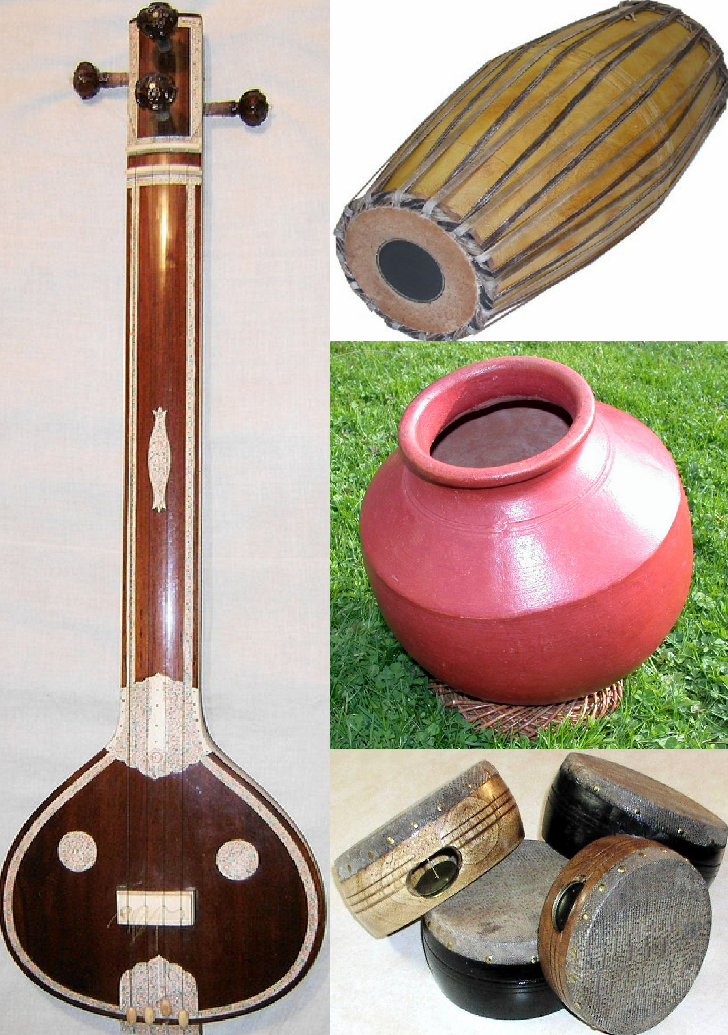
\includegraphics[scale=0.46]{instruments.png}
  \caption{The most popular non-melodic instruments that take part in a concert of carnatic music (Source: Wikipedia). Left: t\=anpura. Top: m\d{r}da\.{n}ga\.{m}. Middle: ghatam. Bottom: kanjira.}
  \label{fig:instruments}
\end{figure}



\section{Musical Elements}

So far, the main ideas and conditions that surround the actual musical elements have been exposed. From the four elements saliented by T. M. Krishna (r\=aga, t\=a\d{l}a, composition and improvisation), this section will describe the r\=aga and t\=a\d{l}a mechanics.\\

A comprehensive explanation of the compositive and improvisatory dimensions of carnatic music is out of the scope of the present thesis, and the details are not needed to understand the concepts presented in chapter \ref{context}. In fact, the carnatic corpus used in the present thesis is compiled based primarily on the r\=aga and t\=a\d{l}a conceps\cite[p.64]{gulati}. Therefore, it won't be covered any further (for that, chapters 5 and 6 of \cite{krishna} are recommended). Some of the reasons have been already mentioned in this chapter: the main difficulty for a systematic approach is one of its core features, the oral tradition itself. In carnatic music, ``at least until the mid-ninetheenth century, the process of composing seems to have been intellectual work passed on orally''\cite[p.72]{krishna}. So a detailled description and analysis of such features would involve a study of all the different schools along their very long history, which is a matter of profound ethnomusicological study by itself. Here, it will suffice to acknowledge that carnatic performances feature high degrees of improvisation, and that this improvisations have some form underlying composed structure that is to be respected by the performers.\\


\subsection{Musical Functions}

As in most traditional repertoires, the constituent elements of the musical discourse have distinct, well-defined functions, that are tightly associated to specific instruments and interpretation practices. Regarding the harmonic dimension, carnatic music can be considered a form of tonal music, since its discourse revolves around a fundamental frequency, fixed along the whole musical piece. In the case of the traditional ensemble, most of the harmonic content (explained later), and especially the fundamental frequency, is provided by the t\=anpura, a mid- to low register string instrument which plays a ``drone'' of sustained notes in the background, and that usually doesn't require a high display of virtuosism to be performed (in fact, there are small electronic devices, the ``electronic t\=anpuras'' that can fullfill this task acceptably).\\

Another functional role in the carnatic ensemble is played by the percussion instruments. They provide a rhythmic basis to the performance by following the t\=a\d{l}a specified by the composition. A t\=a\d{l}a is a ``concrete method of dividing time''\cite[p.63]{krishna} specific to indian art music (more on that later).\\

The most important role in carnatic music, and also the most virtuous one is held by the melodic instruments. They improvise on the played composition following the specified r\=aga, the melodic framework for indian art music (explained later). When having multiple melodic instruments, they form a hierarchy, in which the leader (usually a male or female voice) has a predominant role by having more time and protagonism, and exposing ideas that may be imitated or complemented by the others. Note that although the r\=aga doesn't apply for the percussion instruments, the melodic instruments do have to follow the composition's t\=a\d{l}a, since melody also has rhythmic aspects.

\subsection{R\=agas: The Melodic Framework}

As already said, al the pitched sounds in carnatic music are defined in reference to the fundamental frequency, fixed for the whole performance. This frequency has to be ``carefully chosen by the performer in order to explore the full pitch range effectively in a given rāga rendition''\cite[p.18]{gulati}, so it depends on the performers and is more or less arbitrary.\\

This pitched sounds are organized in the framework of the r\=agas. From \cite{indian-corpora}:\\
``Raga eludes a simple and concise definition, but technically we can say that a raga is a musical entity in which the choice of notes; their order and hierarchy, the manner of intonation of individual notes, relative duration and their specific melodic approach, are clearly defined.''.

More attempts of defining the term can be found in \cite[p.18]{gulati}. As a part of the orally transmitted tradition, every r\=aga has a distinct syntax, that makes it differentiable from the others. But all of them are based on common elements, which are explained hereafter.

\subsubsection{Svaras}

The basic definit element of a r\=aga is given by its supported set of {\it svaras}. ``Every raga has a minimum of five svaras; the maximum is, of course, al seven''\cite[p.53]{krishna}. Svaras are a set of fixed pitch positions\cite[p.46]{krishna} defined as musical intervals in relation to the fundamental frequency, and form the building blocks of the carnatic melody.\\

As in many other musical cultures, the \(2:1\) frequency ratio (known in western music as {\it octave}) works as an identity in many situations, due to its perceived similarity (for example, women sing usually one octave higher than men but learn this system the same way). For this reason, the svaras are defined within one octave and then repeated periodically for every other.\\

Similarly to western music, one octave contains twelve different svaras. Also, as in the case of enharmony or solmisation in western music, where the same note becomes different names depending on the context it is placed in, there are a total of sixteen names for the twelve svaras. And this names are grouped in seven distinct entities: Sa, Ri, Ga, Ma, Pa, Da and Ni. See Figure \ref{fig:svaras} for the specific details.\\

\begin{table}
  \centering
  \resizebox{\textwidth*7/8}{!}{%
    \begin{tabular}{*3c}\toprule
      \bfseries Pitch Position & \bfseries Svara & \bfseries Name\\\Midrule
      1  & Sa      & Shadja (S)  \\\midrule
      2  & Ri      & Shudda Rishabha (R1)  \\\midrule
      3  & Ri2/Ga1 & Chatushruti Rishabha (R2) / Shuddha Gandhara (G1)  \\\midrule
      4  & Ri3/Ga2 & Shatshruti Rishabha (R3) / Sadharana Gandhara (G2)  \\\midrule
      5  & Ga3     & Antara Gandhara (G3)  \\\midrule
      6  & Ma1     & Shuddha Madhyama (M1)  \\\midrule
      7  & Ma2     & Prati Madhyama (M2)  \\\midrule
      8  & Pa      & Panchama (P)  \\\midrule
      9  & Da1     & Shuddha Dhaivata (D1)  \\\midrule
      10  & Da2/Ni1 & Chatushruti Dhaivata (D2) / Shuddha Nishada (N1)  \\\midrule
      11 & Da3/Ni2  & Shatshruti Dhaivata (D3) / Kaishiki Nishada (N2)  \\\midrule
      12 & Ni3      & Kakali Nishada (N3)  \\\bottomrule
  \end{tabular}}
  \caption{The twelve svaras and their sixteen names (from \cite[p.47]{krishna}).}
  \label{fig:svaras}
\end{table}

Depending on the r\=aga, a given svara could belong to one entity or another, and every entity is represented at most by one svara. For example, the Dhany\=asi r\=aga has the Sa=1, Ri=2, Ga=4, Ma=6, Pa=8, Da=9 and Ni=11 svaras, whereas N\=a\d{t}a has Sa=1, Ri=4, Ga=5, Ma=6, Pa=8 and Ni=12: we see that the svara 4 can be Ga or Ri, and that the Da svara is not always present.\\

Among all the entities, Sa and Pa are the only ones that have a unique svara. Sa represents the fundamental frequency in any of its octaves, and Pa represents the \(3:2\) ratio of the fundamental (known as the {\it fifth} in western music), also in any of its octaves. This two svaras correspond to the most basical harmonics of the fundamental and are arguably the most important ones, since both of them are present in practically every r\=aga, Figure \ref{fig:rrd-ragasvaras} is a good example of that. In fact, they can be easily identified in every carnatic piece as they are present in the drone played by the t\=anpura.

\subsubsection{Gamakas}


Although the concept of svara is instrumental to understand hte r\=agas, it has to be noted that ``the svara is a musical form only because of the gamaka [..]. The two concepts are not independent of each other [...]. In other words, the svara does not exist without gamaka''\cite[p.51]{krishna}. But also, that ``the gamaka can be illustrated, can be explained, but it cannot realy be defined. It is described in terms of the svara's oscillation. Gamakas have been explained as melodic ornamentations applied to svaras, giving them mobility around their specific pitch positions''\cite[p.51]{krishna}.\\

This ornamentations are usually microtonal (meaning in western music that they comprise intervals smaller than half tone), and extremely context dependent: specific ornamentations are bound not only to specific r\=agas and gestures, but they can also be tracked to a specific school, artist, or even performance (recall the concept of sampradaya explained before).\\

Despite the difficulty of defining the concept of gamakas in a systematic way, they are an instrumental element of carnatic music. Note that, as the svaras never appear in their pure state, a r\=aga can't be defined just by its set of svaras: the gamakas have to be regarded in every case.


\subsubsection{Ny\=as}

Quoting from \cite[p.19]{gulati}, ``Every r\=aga comprises a set of svaras at which an artist can momentarily pause to release the musical tension built in the melody [...]. The set of svaras on which the pause is permitted in a r\=aga grammar are referred to as ny\=as svaras''.\\

So the ny\=as svaras are also a defining element of r\=agas, but, as the gamakas, they are not trivial to define. Also  from \cite[p.19]{gulati}: ``Typically, occurrence of ny\=as svaras mark the ending of a melodic phrase. A ny\=as is mostly manifested in a melody as a long held svara. However, there are several exceptions to it, which mainly depend on the local melodic context and the global tonal context defined by the r\=aga. R\=aga grammar primarily acts as a guideline, and it does not explicitly define rules for the occurrences of ny\=as in a melody.''

\subsubsection{\=Ar\=ohana and Avr\=ohana}

For this concepts, \cite[p.19]{gulati} offers a very concise and clear description: ``The ascending and descending progression of svaras in a melody of IAM are referred to as \=ar\=ohana and avr\=ohana, respectively. Every r\=aga has a defined constraint on how a melody can progress through its constituent svaras. Thus, \=ar\=ohana-avr\=ohana is a characterizing aspect of r\=agas.''

\subsubsection{Phrases and Chalans}

Similarly to modal melodies in western music, ``every rāga has a set of characteristic melodic phrases that capture the essence of the rāga. These melodic phrases act as a building block to construct melodies''\cite[p.19]{gulati}. Interestingly, this process of creating new melodies by combining preexistent melodic formulas is known as centonization\cite[ch.III]{hoppin}, and is also present in other music cultures like gregorian chant and most notably jazz, which shares with carnatic music the complex relation between compositional and improvisatory aspects.\\

Further quoting from \cite[p.21]{gulati}, ``chalan (literally meaning gait or movement) can be thought of as an abstraction of the melodic phrases. The chalan defines the melodic outline of a rāga, that is, how a melodic transition is made from one svara to another, the precise intonation to be followed during the transition, and the proportion of time spent on each svara''. To provide an intuitive simplification, a phrase can be seen as a chalan with gamaka ornamentations on it.

\subsubsection{Further Considerations}

As seen so far, all the concepts that belong to the core identity of a r\=aga are organically bound one to another, and never appear in their ``pure'' state. And to add more complexity, not every raaga is clearly distinguishable from the others (especially challenging is the case of the allied r\=agas, that ``share a common set of svaras and have a similar melodic phraseology. Typically, these rāgas are differentiated based on subtle melodic nuances and a set of melodic phrases that are specific to them''\cite[p.21]{gulati}). To picture this problematic, figure \ref{fig:carnatic-phrases} shows three different phrases, each one featured by several instances: despite of the evident differences among each group, all the instances are to be identified as belonging to the same phrase.\\

\begin{figure}
  \centering
  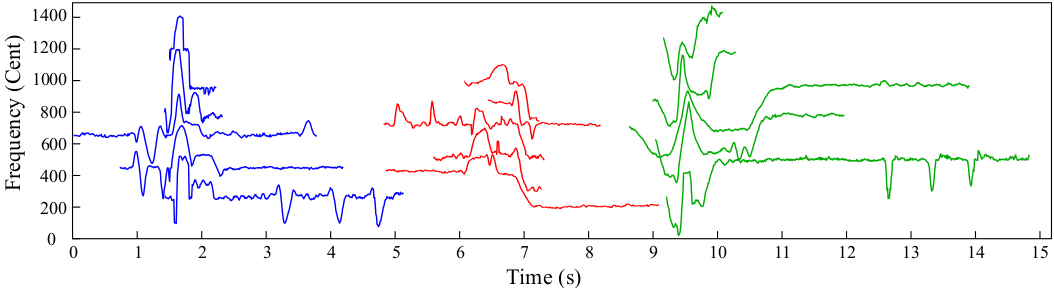
\includegraphics[scale=0.4]{carnatic_phrases.png}
  \caption{Pitch contours of occurrences of three different characteristic melodic phrases in Hindustani music. Contours are transposed in frequency, and shifted in time for a better visualization (from \cite[p.21]{gulati}).}
  \label{fig:carnatic-phrases}
\end{figure}


For all this reasons, r\=aga definition (and therefore also detection and classification) is a highly specialized task that requires a broad domain-specific knowledge, as well as a fine sense. When automating this task, a data-driven approach seems the most reasonable way of tackling it, since, except from the svaras, all the core concepts of a r\=aga can only be defined through context-depended, interconnected sets of examples.


\subsection{T\=a\d{l}a: The Rhythmic Framework}

``Tala is the rhythmic framework governing the temporal aspect of the carnatic music and it can be described as having a certain number of time units or beats (matras) and more importantly sections into which these beats are grouped and stressed''\cite{indian-corpora}.\\

The main difference between the rhythmic frameworks of western and carnatic music (apart from the fact that the latter follows an oral tradition), is that western music subdivides the temporal units from top to bottom, whereas carnatic music does the opposite. Western music follows an approach developed in the Middle Ages, in which each value could be subdivided in three (perfect division) or two (imperfect division) values of equal duration\cite[ch.XIV]{hoppin}. This system naturally evolved to allow more complex relations, but the hierarchical organization remained top down ever since then. Carnatic music builds its rhythmic abstractions by putting together rhythmic elements of shorter duration. Therefore, this section will explain those elements following that order.

\subsubsection{Layas}


Another main difference between western and carnatic music is that the former usually relates the speed to a mathematical value, by taking a specific rhythmic figure and assigning a speed to it, usually in beats per minute. And this speed is basically unrelated to the melodic or harmonic contents that the music may present.\\

In carnatic music, on the other side, ``speed is not equal to an exact mathematical value. It is generally measured as slow, medium or fast (chauka, madhyama, durita). In a generic sense, laya refers to this sense of speed, and is critical to the aesthetics of Karnatik music. The raga form is shaped on the basis of this sense and changes according to this sensed speed''\cite[p.61]{krishna}. Also, the laya of a rhythmic phenomenon ``is not experiencedby a measurable number, but by a general sense of time''\cite[p.61]{krishna}.\\

And further: ``Other tha a general sense of speed, laya also refers to the measure of the interval between every division [...]. When laya comes together with a fixed number of divisions, a composite rhythmic unit, or a tala, is created. A tala is a concrete method of dividing time [...]. Pulsation is found in many places, but it is not considered a tala unless it is created by melody''\cite[p.63]{krishna}.\\

So, after this considerations, it can be said that laya describes a general, emotional sense of rapidness provided by a rhythmic pattern, and only when the pattern becomes predictable and embodies some intentionality can be perceived as a t\=a\d{l}a.

\subsubsection{Kriyas and T\=a\d{l}a Angas}

The predictability of a rhythmic pattern is given by its periodicity: ``Every tala is cyclical in that it repeats its form in exactly the same way right through a composition''\cite[p.63]{krishna}. The layas in this context become then measurable, due to that periodicity, and are known as kriyas.\\

Kriyas are the basic building blocks of a t\=a\d{l}a, and take the form of physical manifestations ``by which both the musician and the listener can identify the tala structure''\cite[p.63]{krishna}. They can be of two types: ``those that make a sound (sashabda kriya), and those that make no sound (nishabda kriya), the first kriya in every tala is referred to as the sama -- the beginning, always the slap on the thigh''\cite[p.64]{krishna}.\\

Kriyas are combined in three structural groups, known as t\=a\d{l}a angas: ``laghu (a slap on the thigh followed by finger counts of 2,3,4,6 or 8 units), druta (a slap on the thigh followed by a flip of the palm) and anudruta (only a slap on the thigh). While druta always has two beats and anudruta one, the laghu is a variable form that can have 3,4,5,7 or 9 beats. This values are essential to all the different tala structures and the laya''\cite[p.64]{krishna}.\\

All the angas have a fixed length, except laghu, that presents ``five j\=atis (categories): chaturashra (with length 4), tisra (length 3), mishra (length 7), khanda (length 5), sankirna (length 9)''\cite[p.64]{krishna}.\\


\subsubsection{Avartanas and T\=a\d{l}as}

The t\=a\d{l}as are formed by combining few t\=a\d{l}a angas into a ``complete tala form called avartana, that is repeated cyclicaly within a specific musical representation''\cite[p.64]{krishna}. If wanting to build an analogy to western music, the role of the avartana would be similar to the measure in a baroque dance suite: the sarabande is a slow dance with has three units (with a stress in the second one) subdivided in groups of two, the gigue is a fast dance with two units (with a stress in the first one) subdivided in groups of three, and so on.\\

``In Karnatik music, there are seven talas that form the basis for the tala structures [...], known as the suladi sapta tala. Most talas in use today are variations of these seven primary talas''\cite[p.64]{krishna}. The suladi sapta talas are pictured in Table \ref{fig:taalas}.


\begin{table}
  \centering
  \resizebox{\textwidth*7/8}{!}{%
    \begin{tabular}{*3c}\toprule
      \bfseries Tala & \bfseries Structure & \bfseries Total\\\Midrule
      Dhruva  & Laghu (4) + Laghu (4) + Druta (2) + Laghu (4)    & 14 \\\midrule
      Matya   & Laghu (4) + Druta (2) + Laghu (4)                & 10  \\\midrule
      Rupaka  & Druta (2) + Laghu (4)                            & 6  \\\midrule
      Jhampa  & Laghu (7) + Anudruta (1) + Druta (2)             & 10  \\\midrule
      Triputa & Laghu (3) + Druta (2) + Druta (2)                & 7  \\\midrule
      Ata     & Laghu (5) + Laghu (5) + Druta (2) + Druta (2)    & 14 \\\midrule
      Eka     & Laghu (4)                                        & 4 \\\bottomrule
  \end{tabular}}
  \caption{The seven primary talas (from \cite[p.65]{krishna}).}
  \label{fig:taalas}
\end{table}



\subsubsection{Final Considerations}

After this considerations, it is fairly safe to say that t\=a\d{l}as are much easier to identify than r\=agas: not only there are much fewer types (as it can be seen in appendix \ref{ds-stats}), but their features are also simpler and much less context-dependent. The identification of the different angas is an easier task compared to, for instance, the gamakas. Given a basic beat of fixed duration, They comprise a fixed amount of beats (among a limited range of options) and they start with a specific gesture, the slap, which is identifiable not only visually but also audibly. When automating this task, there is an added difficulty coming from the fact that not every instrument is repeating the exact same pattern in every avartana, but this can be overcomed by exploiting two main redundancies: first, the periodicity of the avartana itself, which is kept constant thorough the whole piece, and second, the fact that all the instruments of the ensemble are following the same t\=a\d{l}a.


\chapter{Related Work}\label{context}
R\=aga classification belongs to the more general task of music tagging, which is ``one of the fundamental tasks in the field of Music Information Retrieval (MIR)''\cite{stokowiec} and consists of mapping a given audio recording to features attributed to it. Depending on the specific problem domain, this can be a single-label (like r\=aga detection itself) or a multi-label (instrument detection) classification task.\\

To the present moment and to the extent of my knowledge, no successful end-to-end supervised learning research for r\=aga classification was reported. The dominant trend in this field is to apply more domain-specific approaches, which perform well, as as recent work shows, and can be in some cases translated to other domains. Such domain-specific approaches, most notably the research performed by S. Gulati in \cite{gulati}, are  presented in section \ref{context_raaga}.\\

On the other hand, plenty of successful and recent examples of such research with end-to-end, supervised learning setups can be found in the field of Music Genre Recognition (MGR). Also a form of music tagging, MGR is arguably close to r\=aga classification since it shares some of the features and most of the problematic. An overview of the field and the related work is presented in section \ref{context_mgr}.\\




\section{Related Work in Music Genre Recognition} \label{context_mgr}


\subsection{Problematic of the MGR Field}\label{mgr-problematic}

At the moment of writing this thesis, no dataset or approach has been found to be widely accepted as representative of the problem of MGR, as it could be the ImageNet or CIFAR classification contests in the field of Visual Object Recognition (VOR). This could be due to the fact that the idea of genre itself is extremely context-dependent: each musical genre hast its own relevant features, and the degree of differentiation needed for a feature varies a lot from one genre to another. Also, the data is presented in a more abstract form: ``unlike visual image recognition tasks, where outlines of images play an important role, music spectrograms mainly consist of continuous, smooth gradients. There are not only local correlations but also global correlations such as harmonic structures and rhythmic events''\cite{choi-explaining}.\\

Whithout such unified data and error metrics approach, a general benchmarking of the MGR task would be neither possible nor meaningful. And evaluating the state of the art in the MGR field just based on the success of, for instance, western-based contents and genres, would be culturally biased. This is precisely one of the main motivations that led to the foundation of the CompMusic project (as explained in \cite{serra-comp11} and \cite{serra-comp14}), and to the consequent curation of the dataset used in the present thesis (more detais about the dataset can be found in section \ref{about-ds}).\\

B. L. Sturm tackles precisely this problematic in a 2012 survey\cite{mgr_survey}, in which he explores the different initiatives in the MGR field an concludes that ``While genre is an inevitable condition of human communication in general, a way to automatically identify it in music remains elusive''. The reason behind it is the already mentioned context-dependence of the defining features of a genre (or a style, which he considers equivalent), which gets reflected into the variety and diversity of datasets, models and evaluation criteria involved.\\

This said, more recent work has been centered on applying supervised end-to-end setups to systematically explore the context-dependence of musical categories such as genre: K. Choi et al.(2017)\cite{convtransfer} analyzes the performance of convolutional neural networks that have been pre-trained on specific musical categories, when applied on different domains: ``The pre-trained convnet was first trained to predict music tags and then transferred to solve genre classification, vocal/non-vocal classification, emption prediction, speech/music classification, and acoustic event classification''\cite{convtransfer}.\\

\subsection{Comparatives of Different Algorithms}

Among the different datasets reported in \cite{mgr_survey}, one of the most prominent is the Milliong Song Dataset (MSD), a ``freely-available collection of audio features and metadata for a million contemporary popular music tracks''\msdataset. In a 2016 ``Comparative Study on Music Genre Classification Algorithms''\cite{stokowiec} based on this dataset, W. Stokowiec compares ``the performance of various music genre classification algorithms including Random Forests, Multi-class Support Vector Machines and Deep Belief Networks, with an emphasis not only on classification accuracy but also on robustness and scalability of algorithms''. Regarding the results, he observes that ``Random Forests and Decision Trees outperform Multi-class SVM, Multinomial Logistic Regression and naively trained DBN independently of the chosen features, genre dataset or benchmarking partitions. Highest scoring algorithm (Random Forest) trained on dataset with 13 classes reached accuracy of 62\% [...]. In all cases Multi-class SVM had at least 10\% of accuracy less than Random Forest''. But in the case of the deep belief networks (a clase of neural networks, explained in section \ref{neuralnetworks}), he concludes that ``DBN adjustment and optimization'', among other factors, could be an interesting way to explore, since ``in the case of DBN hyperparameter tuning, using grid-search has occurred to be computationally intractable and time constraints become an important issue'', which ``led to unsatisfactory results''.\\

A similar trend regarding the better performance of neural networks for western-based MGR tasks was noticed in 2011 by Haggblade et al.\cite{haggblade}. They also tested different machine learning algorithms, based on four diferent genres of the GTZAN Genre Collection, ``a dataset of 1000 audio tracks each 30 seconds long, with 10 genres represented, each containing 100 tracks''. In it, ``The simpler and more naive approaches, k-NN (supervised) and k-Means (unsupervised), predictably did worse than the more sophisticated neural networks (supervised) and SVMs (unsupervised)''. As a curiosity, it is interesting to remark how the landscape has shifted since then: ``we expected similar performance from SVMs and neural networks based on the papers we read, so the significant superiority of neural networks came as a surprise''.\\


\subsection{Data Representation}

It is interesting to note that the MSD does not contain audio recordings: due to licensing issues, it ``provides precomputed features instead of raw audio [...]. Unfortunately, some authors [9] claim that the absence of accurate documentation of the extraction algorithm renders the audio features provided by MSD of limited use.''\cite{stokowiec}. Other datasets, as the already mentioned GZTAN, do provide the recordings, but in smaller scale. This contrasts with the data curated in the context of the CompMusic project (as the carnatic dataset used in this project and described in chapter See \ref{about-ds}), which doesn't present any of this disadvantages.\\

Regarding the explicit focus on representations in the context of the end-to-end MGR, most of the research done up to 2017 (like \cite{ireland-mfcc}, \cite{haggblade}, \cite{belgium-mfcc} or \cite{choi-robustness}) is based on time-frequency representations of the sound (explained in section \ref{timefreqrepr} of the present thesis).\\

Back in 2011, researchers from the University of Montreal and Google posed the question wether MFCC deserved its popularity in the MGR field: ``Many automatic annotation systems use features such as MFCCs because they have shown their worth in the speech recognition domain. However, music audio is very different from speech audio in many ways. So, MFCCs, which have been engineered for speech analysis might not be the optimal feature to use for music audio analysis''\cite{montreal-mfcc}.\\

But the fact is that they are still very popular. The current situation to this respect is very well summarized in \cite{choi-robustness}: ``STFT and melspectrogram have been the most popular input representations for deep learning for music. Melspectrograms provide an efficient and perceptually relevant representation compared to STFT and have been shown to perform well in various tasks. However, an STFT is closer to the original signal and neural networks may be able to learn a representation that is more optimal to the task. This requires large amounts of training data however [...]: using melspectrograms outperformed STFT with a smaller dataset''.\\

Interestingly, recent work seems to have found a solid reason for that: Lee et al\cite{wavdeep} showed this year that deep convolutional neural networks (DCNN) trained with raw waveforms ``are sensitive to log-scaled frequency along layer, such as mel-frequency spectrogram that is widely used in music classification systems''. In other words: the networks trained on raw waveforms tend to invest more of their representational capacity into the frequencies that are more important to the human ear according to the mel scale (see Figure \ref{fig:wav-to-mfcc} for a visualization of the trained weights, and Figure \ref{fig:melscale} for a plot of the mel scale).\\

\begin{figure}[h]
  % \hspace*{-0.6cm}
  \centering
  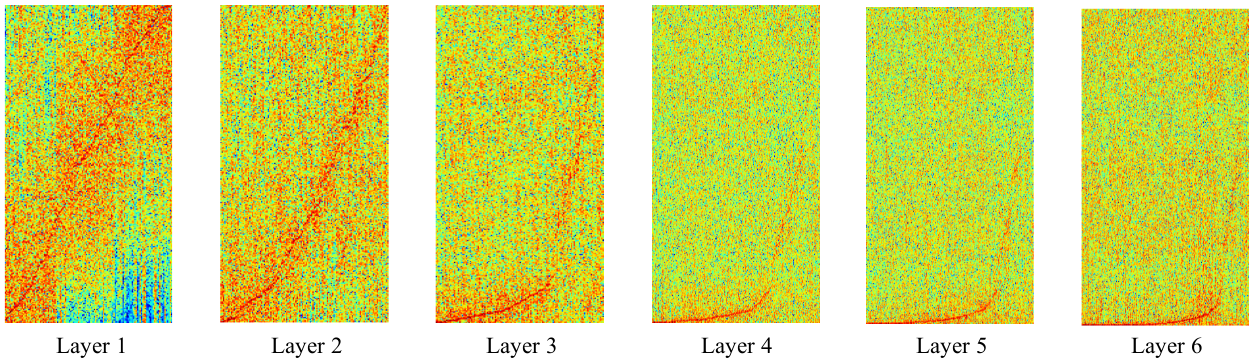
\includegraphics[scale=0.34]{wav_to_mfcc.png}
  \caption{``Spectrum of the filters in the sample-level convolution layers which are sorted by the frequency of the peak magnitude. The x-axis represents the index of the filter, and the y-axis represents the frequency'' (from \cite{wavdeep}).}
  \label{fig:wav-to-mfcc}
\end{figure}



\subsection{Models and Architectures}

Following the general trend suggested by the aforementioned comparatives (and observed in many other fields of the machine learning discipline), research based on the application of deep neural networks for end-to-end supervised learning for perceiving and predicting high-level musical features has observed a growth in quantity and success in the last years.\\

For instance, Lambert et al. combined in 2015 a network of non-linear oscilators with a deep recurrent neural network to sucessfully perceive and predict expressive rhythms\cite{expressive-rhyt}.\\

More specifially to MGR, the team of Choi et al. at the Centre for Digital Music of the Queen Mary University of London has been focusing in developing, implementing, testing and interpreting different deep learning approaches for the last few years. From their work in 2017 so far, apart from the already mentioned work reported in \cite{convtransfer} and \cite{choi-robustness}, it is worth to highlight a very interesting article in which they discuss novel techniques and approaches to interpret the process of learning and predicting high-level musical features by DCNNs\cite{choi-explaining}, especially the idea of auralisation.\\

Regarding specific architectures, they presented last year several fully-convolutional models \cite{choi-fcn}, able to learn high-level features from different domains ``such as emotion (sad, anger, happy), genre (jazz, classical) and instrumentation (guitar, strings, vocal, instrumental)'' on two different datasets, and perform multi-label tagging on them with a top performance of 0.851 AUC-ROC, which is a figure of merit that takes both precision and recall into account (see section \label{errormetrics} for more information).\\

\begin{figure}[h]
  % \hspace*{-0.6cm}
  \centering
  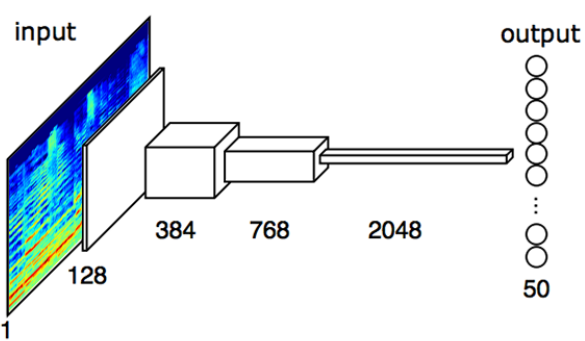
\includegraphics[scale=0.5]{fullyconv.png}
  \caption{One of the fully-convolutional neural architectures proposed in \cite{choi-fcn}. The numbers indicate the number of feature maps (i.e. channels)}
  \label{fig:wav-to-mfcc}
\end{figure}


Two months after, they presented for the same task a convolutional recurrent neural network (CRNN)\cite{choi-crnn}, which combines ``(CNNs) for local feature extraction and recurrent neural networks for temporal summarisation of the extracted features''. In the experiments they observed ``a trade-off between speed and memory: the computation of the purely convolutional network is faster than that of CRNN across all parameter settings, while the CRNN tends to outperform it with the same number of parameters''.









\section{Related Work in Carnatic R\=aga Classification} \label{context_raaga}

The task of r\=aga classification presents similar problems to the ones already exposed in section \ref{mgr-problematic} for the music genre classification: as explained by S. Gulati in 2016, ``the datasets used for evaluation by the existing methods vary immensely in terms of the number of r\=agas, the chosen set of r\=agas, the duration and the number of the audio recordings per r\=aga, and the type of audio content (monophonic or polyphonic). With such diverse datasets, it is difficult to draw any concrete conclusions on the performance of the methods across different studies. Even the survey studies such as those in Koduri et al. (2011) have not performed any exhaustive comparative evaluations on the same dataset and under the same experimental setup. Thus, creating diverse, sizable and sharable datasets that are representative of the music tradition is a potential avenue for contribution in this task. In addition to the datasets, poor description of the implementation details is another common factor amongst several existing studies. This situation becomes even more difficult as none of the approaches make their code publicly available for ensuring reproducibility of the research results''\cite[p.44]{gulati}.\\


For this reason, he opts to ``refrain from comparing the absolute r\=aga recognition accuracies across studies''\cite[p.37]{gulati}. Following this criterium, the present section will be focused on his work, since it is the most relevant for the present thesis: both this and his work are based on the same dataset, from which he is not only one of the curators (see \cite{indian-corpora}) but also its most relevant contributor to the moment. Furthermore, the dataset is ``to the best of our knowledge the largest ever used for this task''\cite[p.178]{gulati} (see chapter \ref{about-ds} for more details on the dataset).\\

Specifically, the two following sections describe ``two novel approaches for rāga recognition that jointly capture the tonal and the temporal aspects of melody'', developed by him in the context of his 2016 dissertation at the Universitat Pompeu Fabra in Barcelona. Finally, some applications of his work are also mentioned. A detailed summary of the work preceding Gulati's can be seen in Figure \ref{fig:gulati-related}.

\begin{sidewaysfigure}%[h]
  % \hspace*{-0.6cm}
  \centering
  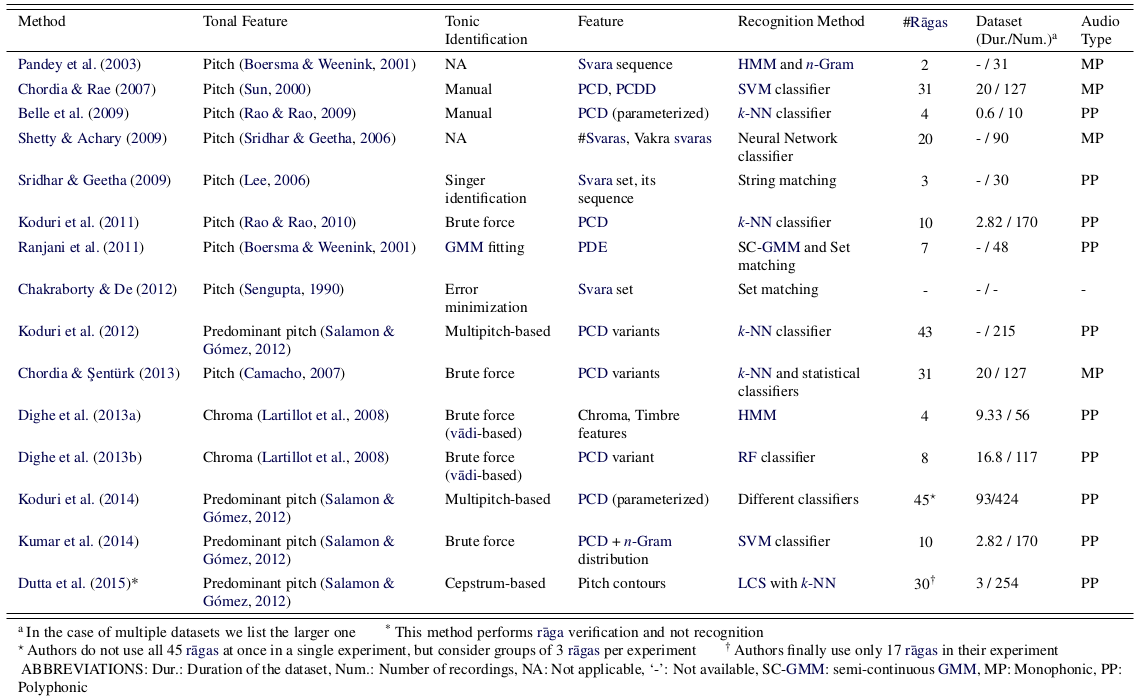
\includegraphics[scale=0.57]{gulati_related.png}
  \caption{Summary of the r\=aga recognition methods in cronological order (from \cite[p.39]{gulati})}
  \label{fig:gulati-related}
\end{sidewaysfigure}



\subsection{Vector Space Modelling (VSM) Approach}

The first approach ``employs concepts of vector space modelling to perform r\=aga recognition using melodic patterns''. It is divided in three parts: first, the audio is sent through a pipeline that is able to identify melodic patterns by extracting specific audio features. This patterns are then clustered when they are considered ``different occurrences of the same underlying melodic phrase''. Finally, and similarly to word embeddings in the text-technology field, the different clustered phrases are considered as elements of the vocabulary, and their sequence of appearance is modelled as a vector, which is finally used to detect a specific r\=aga by the type and frequency of appearance of its elements.\\

This model ``shows promising results by achieving an accuracy comparable to the state of the art method'' and ``has several advantages such as musically meaningful interpretation of the classification results''\cite[p.191]{gulati}. For instance, its experimental results ``suggest that, considering just the presence or the absence of a melodic pattern, irrespective of its frequency of occurrence, might be sufficient for r\=aga recognition. Interestingly, this finding is consistent with the fact that characteristic melodic patterns are unique to a r\=aga and a single occurrence of such patterns is sufficient to identify the r\=aga''\cite[p.186]{gulati}.\\


\subsection{Time Delayed Melodic Surface (TDMS) Approach}

This approach ``uses a novel feature, the time delayed melodic surface (TDMS). TDMS captures tonal and temporal melodic aspects that are useful in characterizing and distinguishing rāgas. TDMSs alleviate several of the shortcomings in the existing approaches and improves the accuracy of r\=aga recognition by large margins, without the use of any elaborated classification schema''. The only drawback for that is that it ``seeks to abstract the melody representation'', giving up some of its interpretability.\\

As explained in\cite[p.192]{gulati}, the computation of a TDMS involves three steps: pre-processing (which normalizes a low-level representation of the melody with respect to the tonic pitch), surface generation (a two-dimensional discretized histogram of the elements of the pre-processed melody), and post-processing (consisting on applying some compression and smoothing to the surface). Figure \ref{fig:tdms} shows an example of such surface, before and after post-processing.\\

All the proposed variants of this method scored at least 81.5\% of accuracy when applied to the 40 r\=agas of the \(RRD_{CMD}\) dataset (described in chapter \ref{about-car}).


\begin{figure}[h]
  \centering
  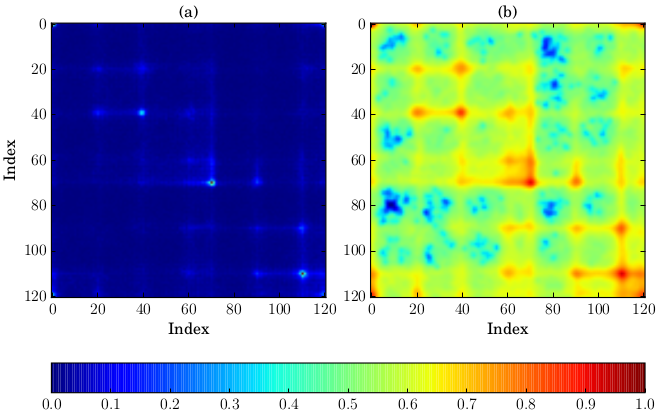
\includegraphics[scale=0.5]{tdms.png}
  \caption{An example of the generated TDMS for a music piece in r\=aga Yaman, before (a) and after (b) applying post-processing (from \cite[p.195]{gulati})}
  \label{fig:tdms}
\end{figure}


\subsection{Applications}

The results of Gulati's work have already found several applications. One of them is the {\it raagawise}\cite{raagawise} web-application, which performs r\=aga recognition based on an incoming audio stream. Another remarkable one is the tonic identification software present in the Dunya platform (described in section \ref{compmsc}). Figure \ref{fig:dunya-player} shows a screenshot of the platform's audio player, wich besides the raw audio wave displays its extracted melodic and spectral features.

\begin{figure}[h]
  \centering
  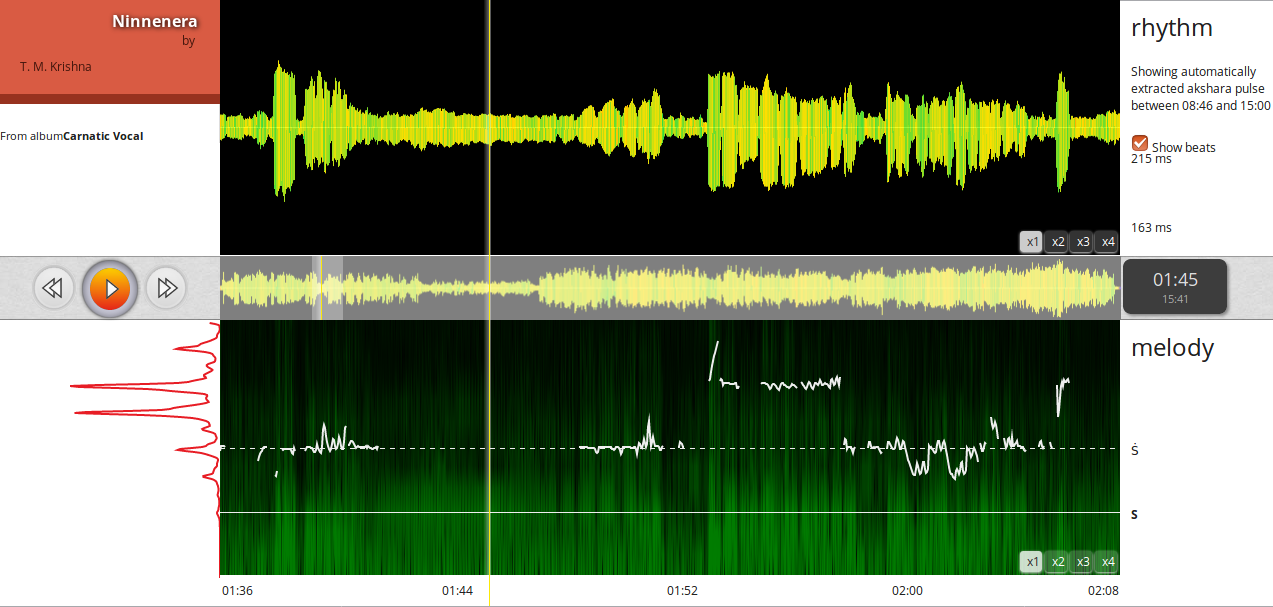
\includegraphics[scale=0.33]{dunya_player.png}
  \caption{A screenshot of the main section of Dunya's music player. Note the extracted melodic and spectral features.}
  \label{fig:dunya-player}
\end{figure}
 

\chapter{About Machine Learning} \label{about-ml}
As already anticipated in the summary, the present thesis implements a supervised learning model for music classification. This chapter will cover the technical basis necessary to have a sound understanding of the model, following the mindmap provided in figure \ref{fig:mindmap}.

\begin{figure}[h]
  \hspace*{-0.6cm}
  \centering
  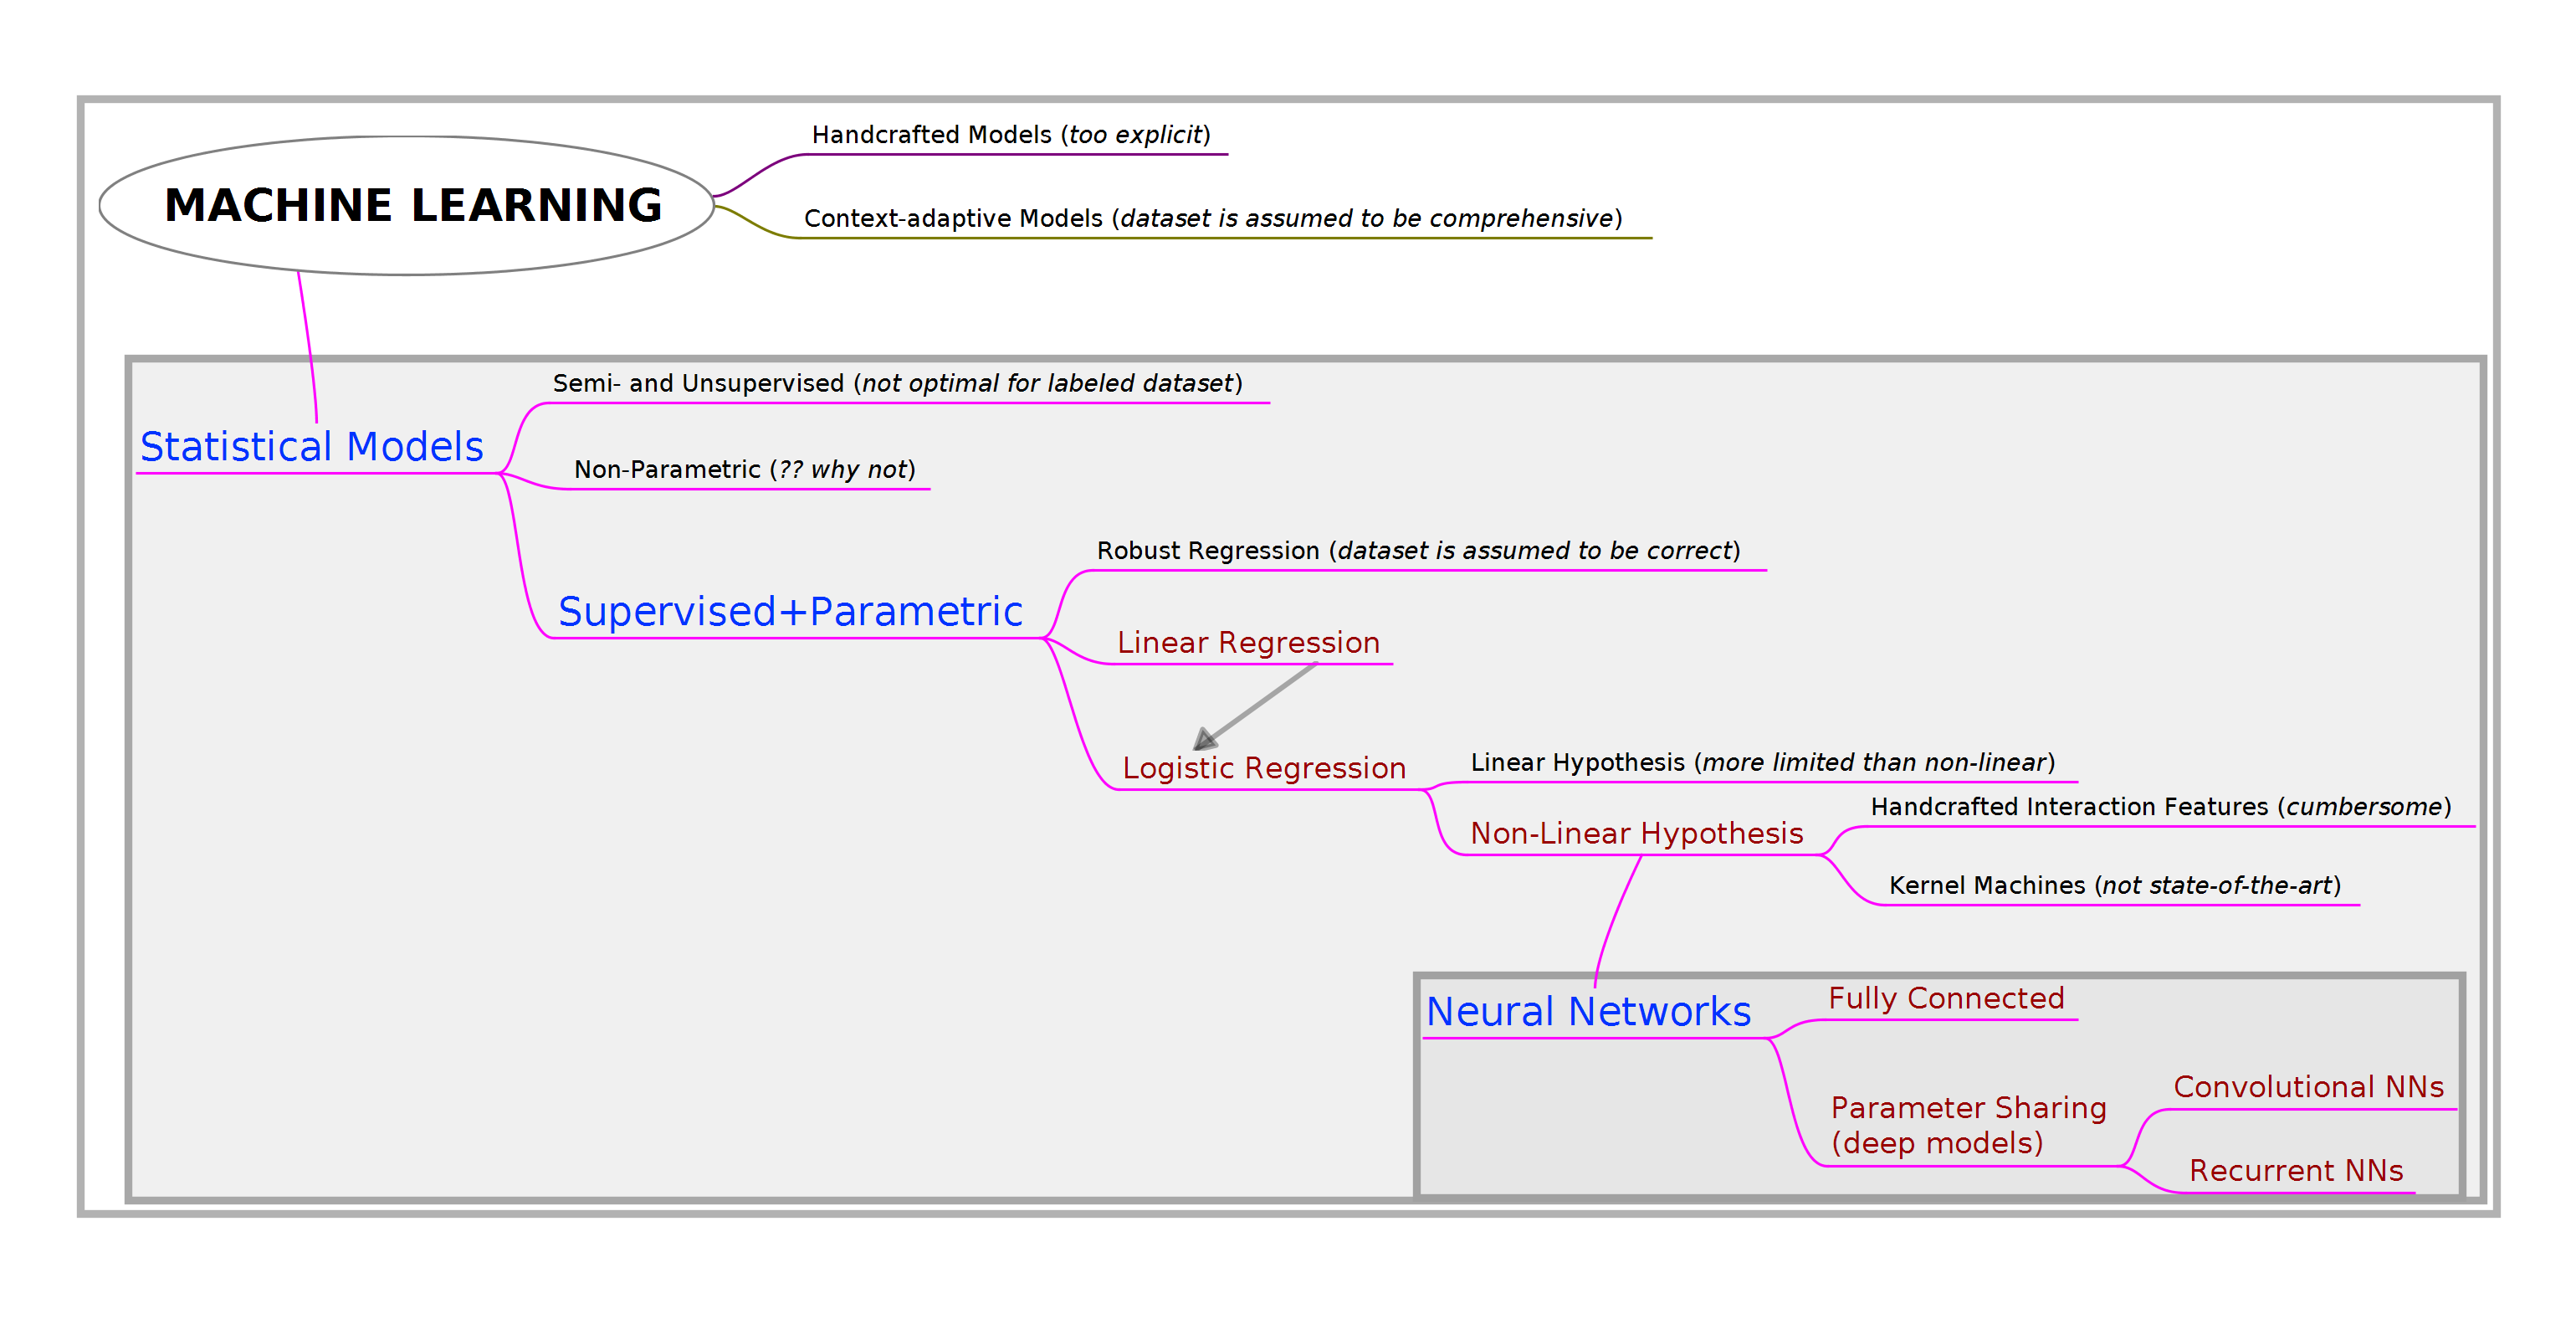
\includegraphics[scale=0.6]{freeplane/machine_learning.png}
  \caption{A mindmap of this chapter's contents. The concepts in the smallest font weren't used in this project, and are covered just enough to understand why (a small explanation can be found in the parentheses).}
  \label{fig:mindmap}
\end{figure}


The mindmap covers some machine learning models, building up from very simple mathematical concepts to the state of the art models for classification. But although deep learning is a specific kind of machine learning\cite[p. 98]{goodfellow}, it doesn't mention the word deep, for a reason: When a machine learning model is structured in hierarchical layers (like neural networks), it is possible to talk about its {\it depth}. In this context, {\it deep} learning models (as opposed to {\it shallow} models) are machine learning models with many layers. But the fact is that ``there is no single correct value for the depth of an architecture, nor is there a consensus about how much depth does a model require to qualify as {\it deep}''\cite[p.8]{goodfellow}. Also, it is much more reasonable to structure the chapter contents based on the mathematical techniques that the different models are based on, rather the exact number of implemented layers.\\


In fact, the depth of the model plays a very relevant role not only from a technical point of view, and there is much support to claim that ``Deeper models tend to perform better''\cite[p.202]{goodfellow}. The concept of {\it deep learning} is fairly new, dating from 2006\cite[p.13]{goodfellow}, but the practice has actually decades of rich history (there are many divulgative texts covering the history of deep learning in further detail, notably \cite{deephist} and also \cite[p.13]{goodfellow}).\\



\section{Machine Learning}

The main idea of machine learning was already formulated by Turing in 1950, with the idea of the {\it child programme} and the education process\cite{turing:50}: based on this idea, some steps in the solving process are automatically inducted from a given dataset instead of hardcoded. But this definition is very broad, and encompasses well over 60 years of history (some core techniques like the {\it least squares optimization} trace back to Gauss' times\cite{lso}), covering a wide amount of paradigms, structures, techniques and concepts used in many different applications. Tom M. Mitchell provided in 1997 a much more specific concept of learning applied to machines\cite[p.99]{goodfellow}:
\begin{quote}
  A computer program is said to learn from experience E with respect to some class of tasks T and performance measure P , if its performance at tasks in T , as measured by P ,improves with experience E.
\end{quote}
The advantage of this definition is that it involves a fairly simple set of elements, and expresses the rather complex task of learning as a relationship among them that not only is conceptually very elegant, but also very practical. It also seems to be widely accepted, being directly used in \cite{goodfellow} and \cite{coursera-ml}, and indirectly in \cite{russell}. But the fact is that it still encompasses a very broad range of AI techniques. John Launchbury, a director of the {\it Defense Advanced Research Projects Agency} (DARPA) has released very recently a brief Perspective on Artificial Intelligence\cite{darpa-slides}-\cite{darpa-vid}, in which he provides a more comprehensive and structured view. In it, he defines artificial intelligence as the ``{\it programmed} ability to process information'', that can be decomposed in a set of four skills: \textbf{perceiving}, \textbf{learning}, \textbf{abstracting} and \textbf{reasoning}. Based on this, he distinguishes 3 historical ``waves of AI'':
\begin{enumerate}
\item Handcrafted Knowledge (characteristical task: {\it describe}): ``Engineers create sets of rules to represent knowledge in well-defined domains. The structure of knowledge is defined by humans, the specifics are explored by the machine''. An example of this are the classical Chess AIs. This models have high capacity of reasoning, a minimal perceiving of the environment, and no learning or abstracting capability.
\item Statistical Learning (characteristical task: {\it categorize}): ``Engineers create statistical models for specific problem domains and train them on big data.''. In some cases, it is very difficult or impractical for humans to define a problem domain as an explicit set of rules, but much easier to collect a set of examples that implicitly responds to those rules. This kind of models are able then to learn an explicit representation of those rules by inspecting the dataset (ref manifold): as opposed to the deductive nature of the first-wave models, statistical models base their learning on induction. They are great in perceiving the environment and learning from it, but have poor abstracting and reasoning capabilities. As a consequence, ``this models are individually unreliable: inherent flaws can be exploited and skewed training data creates maladaptation''(see figure \ref{fig:panda}). So for them to success, the selection of the data has to be carefully done by humans, and even in that case they are exposed to flaws like the shown in figure \ref{fig:panda}, because the representation that this models learn is in most cases too abstract to be directly interpreted. Hence, the model architecture can only be validated by trial and error, they are treated as black boxes, and their training process is considered an ``end-to-end'' one. This makes very problematic to use them in critical domains, where it is very important not only to have a good overall success rate, but also to be able to handle anomalies consistently ``in such a way that the secret of the mechanism are revealed, with no surprises left [...]. Disregard of this principle has not infrequently led to disaster''\cite[p.436]{controlsystems}. A more recent case covering the so-called {\it adversarial examples} can be found in \cite{adversarial}.\\
  Nevertheless, statistical models are widely used and conform the state of the art for many problem domains. Artificial neural networks belong to this category.
\item Contextual Adaptation (characteristical task: {\it explain}): ``The (future) third wave of AI, comprises systems that construct contextual explanatory models for classes of real world phenomena: Understand why/why not, know when will success/fail, know when to trust it, know why it failed''. This is the kind of knowledge that addresses the problems derived from the black-boxed nature of the second-wave models, but not only that: They are as capable to perceive and learn from the environment, but in a way such that the inferred categories have an explicit semantics, and therefore can be combined for further reasoning and abstracting. The drawback of this approach is that, in contrast with the second-wave models, the development and application often involves a more complex methodology and higher computational costs.
\end{enumerate}

\begin{figure}[h]
  \centering
  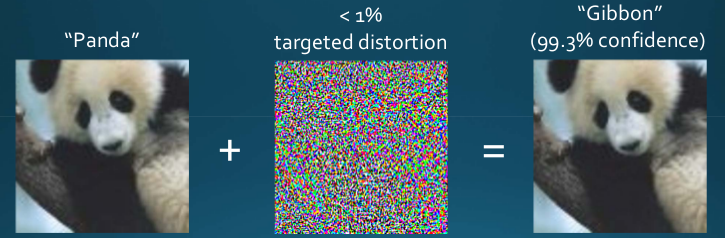
\includegraphics[scale=0.6]{panda-gibbon.png}
  \caption{From \cite{darpa-slides}: Example of the inherent flaws of statistical models: for the human eye, the distorted panda looks almost identical to the original; whereas the trained model predicts a gibbon.}
  \label{fig:panda}
\end{figure}


%% The question wether artificial intelligence is limited to information processing, and/or measured by a combination of those four skills is matter for an interesting discussion, but arguably out of the scope of this thesis. In any case, the points exposed so far enable a way to contextualize and justify the approach taken in this project, namely to use artificial neural networks for music classification:

%% \begin{itemize}
%%         \item As in most art forms, music categories aren't a well-defined problem domain, except for the most trivial cases (and carnatic music is definitely not one of those). So the first-wave approach is discarded: it would be extremely impractical (at best) to attempt to define a rule-based algorithm that describes such complex categories comprehensively.
%%         \item Assuming that no life-critical task would depend on music classification, and that there isn't a systematic to establish that a piece of carnatic music is more relevant than the others, the overall classification success rate is arguably a good measure for the model's success. Following this criteria, statistical models are not excluded.
%%         \item Furthermore, in this project is also assumed that the dataset is comprehensive, correctly labeled, and that carnatic music didn't experience any radical change in the last century. Based on this assumptions, contextual adaptation would be desirable, but not required and third-wave models aren't needed to correctly perform classification on the dataset. It would also follow that the results on the dataset are extrapolable for any kind of current or recorded carnatic music. Of course, this are very strong assumptions and can severely skew the conclusions, but the curation of a dataset or the expertise in the history of carnatic music are matters outside the scope of this thesis.
%%         \item The Dunya dataset is fairly recent, and hasn't been fully explored yet. The range of applications where deep learning models outstand is steadily growing (they conform the state of the art for many classification problems), and the question on how do they perform on that dataset is {\it per se} a legitimate one.
%%         \item Last but not least, there are also practical considerations: statistical models are currently a relevant technology and a sound knowledge on how to design and apply them is not only desirable, but also necessary before critizising and improving them. Context-adaptative approaches are also desirable, but would require sound knowledge in more advanced techniques like covariance propagation, bootstrapping and others that would be more suitable in the context of a more advanced study level.
%% \end{itemize}




\section{Supervised Learning}\label{supervlearning}

As already mentioned, identifying an example as belonging to a category is sometimes much easier as defining the category itself. In that case, the categories can be implicitly defined as a collection of labeled examples, by doing this comprehensively. It is also possible for statistical models to learn categories from a dataset with few or even no labels, by performing unsupervised and semi-supervised learning. But if the dataset has been already labeled (and is assumed to be correct, consistent and comprehensive, as in this thesis), it is more sensible to perform supervised learning, since it profits the most from the extra information provided by each sample's label.\\

This section will describe the general features of every parametric model performing supervised learning, as well as the main strategy to follow: maximizing the likelihood.

\subsection{Setup Formalization}

The task of supervised learning, as described in \cite[Chapter 18]{russell}, is:
\begin{quote}
  Given a \textbf{training set} \((X, y)\) of \(m\) input-output pairs \( (x^{(1)}, y^{(1)}), (x^{(2)}, y^{(2)}), ...  \) \((x^{(m)}, y^{(m)}) \), where each \(y^{(j)}\) was generated by an unknown function \(y = f(x)\), discover a function \(h\) that approximates the {\it true function} \(f\).
\end{quote}
Where each \(x^{(i)}\) is a \textbf{feature vector} in \(\mathbb{R}^n\), having \(n\in\mathbb N_{> 0}\) dimensions (the \textbf{features}) and elements labeled from \(x_1^{(i)}\) to \(x_n^{(i)}\). This specifical kind of dataset is also called labeled, because each \(x^{(i)}\) is coupled to its \textbf{label} \(y^{(i)}\in\(\mathbb{R}\)\). The compact notation \((X, y)\) is used here to refer to the whole dataset, being \(y\in\(\mathbb{R}^m\)\) the vector of labels and \(X\in\mathbb{R}^{m\times n}\) the matrix holding all \(x^{T}\) feature vectors.\\
The defining characteristic of supervised learning is that it is always based on labeled data, and it has two main applications: \textbf{regression}, where \(y^{(i)}\) and the output of \(h\) are real numbers, and \textbf{classification}, where they are discrete. The possible outputs of a classificator are called \textbf{classes}.\\

In this context we define a \textbf{model} where \(h(\theta, x)\) (usually called the \textbf{hypothesis} function) has some \textbf{parameters} or \textbf{weights} \(\theta\) and combines them with the \textbf{input} \(x\) to make its \textbf{prediction}. If there is only a limited set of weights, the model is called \textbf{parametric}. The goal of the training is to adjust those parameters so that \(h\) ends up as close as possible to \(f\). And to get those parameters ``better'' it is needed at first point a criterion to know how ``good'' they are. This is given by the \textbf{cost function} \(J(\theta, X, y)\) (also called \textbf{objective}, \textbf{loss} or \textbf{error} function indistinctly), that performs some kind of comparation between each \(h(\theta, x^{(i)})\) and its respective \(y^{(i)}\), and outputs a non-negative real number representing how bad \(h\) behaves. This number can be interpreted as the ``distance'' between the hypothesis and the true function.


\subsection{Optimization Strategy}

Once we have \(J\) as a way to measure the quality of the parameters, the problem turns into a numerical optimization one, namely:
\begin{equation*}
  \begin{aligned}
    & \theta^* = \underset{\theta}{\text{minimize}}
    & & J(\theta, X, y)
  \end{aligned}
\end{equation*}
Where the best parameters (\(\theta^*\)) are the ones that afford the minimal value of \(J\) for the given dataset. This means \(J\) is used in the model as a criterium not only to \textbf{evaluate} but also to \textbf{learn}.\\

It is important to remark that coming up with a good \(J\) isn't a trivial task: its criterium must be formulated in a concise but general way, but on the other hand it must be kept computationally simple since it must be usually applied many times on big amounts of data. The optimization of \(J\) is also rarely trivial (see \ref{graddesc} for more details and an explanation of the \textbf{gradient descent} algorithm, used in most settings and also in this project for the optimization of \(J\)). For all this reasons, the cost function is one of the most characteristical and important features of a learning model.\\

In this context, and always quoting from \cite[p.131]{goodfellow}: ``Rather than guessing that some function might make a good estimator, we would like to have some principle from which we can derive specific functions that are good estimators for different models. The most common such principle is the \textbf{maximum likelihood principle}.''
``One way to interpret maximum likelihood estimation is to view it as minimizing the dissimilarity between the empirical distribution p̂ data defined by the training set and the model distribution, with the degree of dissimilarity between the two''.

If X represents all our inputs and Y all our observed targets, then the conditional maximum likelihood estimator is:

\begin{equation*}
  \begin{aligned}
    & \theta_{ML} = \underset{\theta}{\text{maximize}}
    & & P(y | X, \theta)
  \end{aligned}
\end{equation*}

And if the examples are assumed to be independent and identically distributed (as we assume for our dataset), then this can be decomposed into:
\begin{equation*}
  \begin{aligned}
    & \theta_{ML} = \underset{\theta}{\text{maximize}}
    & & \sum_{i=1}^m log P(y^{(i)} | x^{(i)}, \theta)
  \end{aligned}
\end{equation*}


Under the right conditions, the main appeal of the maximum likelihood estimator is that it can show \textbf{consistency} (meaning that as the number of training examples approaches infinity, the maximum likelihood estimate of a parameter converges to the true value of the parameter) and \textbf{efficiency} (meaning that compared to other estimators, it will require fewer examples to obtain a fixed level of generalization error). See \cite[p.134]{goodfellow} for a more detailed explanation.


\subsection{Caveats}

The provided explanation so far applies to all the supervised learning techniques explained in the following subsections. Note that it is exposed to many other problems apart from the already mentioned, for instance:
\begin{itemize}
\item It doesn't regard if the modelled \(h\) is complex enough to be able to emulate \(f\), this is something that the designer must care about. On the other hand, if the model is too complex, it may tend to simply memorize the training examples and fail to generalize well, a problem known as \textbf{overfitting}.
\item Even if the model seems adequate, a bad management of the data (for example, testing on the same data that was used to train) or an inconsistent dataset may strongly skew the outcome.
\item Many models are also very sensitive to how the data is formatted, and some simple preprocessing may be recommendable or even necessary (for example, normalizing the data before performing a PCA compression).
\item The total cost or the success ratio aren’t always appropiate ways to measure performance. For example, if some detection problem has only 0.001\% positives, simply assigning every case to negative would provide a 99.999\% accuracy without being useful at all.
\end{itemize}





%%    \section{Linear Regression}\label{linearreg}
%%    This category comprises the regression techniques that base their hypothesis function on a \textbf{dot product} between the input vector \(x\) (passed to some function \(\phi\)) and a parameter vector \(\theta\) of the same dimensionality. It can be thought as ``a sum of elements in the input vector weighted by elements of the parameter vector''\cite[ch. 10.1]{cohen}. In its simplest form, sufficient for this explanation, \(\phi\) is the identity function \(\phi(x)=x\) and can be omitted (alternative strategies for \(\phi\) and their motivations will be discussed in \ref{interaction}). The remaining dot product is a linear function that can be intuitively seen as an ``affinity filter'' between the to-be-learned \(\theta\) vector and the given features, producing its predicted, real-valued output. This is the core idea and that's why it is called linear regression. Actually, what \(h\) performs is an \textbf{affine function}, that is, the explained linear transformation followed by a translation. This translation is necessary to approximate functions with constant components, and is achieved by adding a \textbf{intercept} or \textbf{bias term} \(b\) to the dot product:\\
%%    \begin{equation*}
%%      h(\theta, b, x) = \theta^Tx+b
%%    \end{equation*}

%% Some languages and libraries allow to write this operation directly in this algebraic (so-called \textbf{vectorized} form: for more on vectorization see \ref{vectorization}). Also, for the sake of notation brevity, and as explained in \ref{implicitbias}, this work will use the following {\it implicit bias} notation as equivalent:

%%    \begin{equation*}
%%      h(\theta, x) = \theta^Tx
%%    \end{equation*}


%% \subsection{Hypothesis Function}

%% The simplest case takes place when the input has only one feature (for example, predict the weight of a person based on the height). The hypothesis is in its expanded form \(h(\theta, x)=\theta_0+\theta_1x\), and implies that the model is expected to work well when the {\it true function} behaves close to linearly (example: see figure \ref{fig:unilinreg_b}). In fact, it will reach zero cost if and only if all the points of the dataset are alligned, or ``collinear''.\\

%%  Multivariate linear regression, as the name suggests, applies when the input vector has more than one dimension. For example, predict the prize of a car based on its many features: length, color, horsepower... although an univariate approach based only on the horsepower would probably be effective, taking more features helps to make preciser predictions. It can be intuitively seen as the simultaneous learning of many univariate linear regressions, where all bias terms add up to a single \(\theta_0\), since all of them share the same ``bias feature'' (\(x_0=1\)), and all the other terms are linearly independent from each other. Again, the expanded form of the hypothesis for \(n\) features is: \(h(\theta, x) = \theta_0+\theta_1x_1+\cdots +\theta_nx_n\).


%% \subsection{Cost Function and Optimization Objective}

%%    The linear basis explained so far has the advantage of being stable, and computationally very efficient, especially when combined with the \textbf{mean squared error} (also referred as the \textbf{MSE}, \textbf{L2} or \textbf{euclidean}) cost function: as the name says, it measures the mean of the squared distance between the hypothesis function and the labels. The optimization objective is to minimize it is known as the \textbf{least squares estimation} ({\it LSE}):
%%    \begin{equation*}
%%      \begin{aligned}
%%        & \underset{\theta}{\text{minimize}}
%%        & & J(\theta, X, y) = \frac{1}{2m}\sum_{i=1}^m\{(h(\theta,x^{(i)})-y^{(i)})^2\}
%%      \end{aligned}
%%    \end{equation*}

%% The computational efficiency becomes evident by the fact that the derivative of a square function is a linear function itself. In fact, the \(\frac{1}{2}\) factor is there simply to make the derivative used in the gradient descent equation of \(J\) even more straightforward, as shown below:

%%   \begin{tcolorbox}[ams align*]

%%                The derivative for the mean squared error with respect to a parameter \(\theta_j\) can be calculated following this derivation rules:
%%              \begin{align*}
%%                \begin{aligned}
%%                  &(f(z)+g(z))' = f'(z) + g'(z)\\
%%                  &(f(z)g(z))' = f'(z)g(z) + f(z)g'(z)\\
%%                  &(f(g(z)))' = f'(g(z))\cdot g'(z)\\
%%                \end{aligned}
%%              \end{align*}
%%              Where, in the case of \(J(\theta, X, y) = \frac{1}{2m}\sum_{i=1}^m\{(h(\theta,x^{(i)})-y^{(i)})^2\)\}
%%              \begin{align*}
%%                \begin{aligned}
%%                  & \frac{\partial \frac{1}{2m}}{\partial \theta_j} = 0\\
%%                  & \frac{\partial (\theta^Tx^{(i)}-y^{(i)})^2}{\partial \theta_j} = 2(\theta^Tx^{(i)}-y^{(i)})\cdot x_j^{(i)}\\
%%                \end{aligned}
%%              \end{align*}
%%              Therefore, it holds:
%%              \begin{align*}
%%                \begin{aligned}
%%                  \frac{\partial \(J(\theta, X, y)}{\partial \theta_j} &= \frac{1}{2m} \cdot 2 \{\sum_{i=1}^m(\theta^Tx^{(i)}-y^{(i)})\cdot x_j^{(i)}\}\\
%%                  &= \frac{1}{m} \{\sum_{i=1}^m(\theta^Tx^{(i)}-y^{(i)})\cdot x_j^{(i)}\}\\
%%                \end{aligned}
%%              \end{align*}   % ( \big( \Big( \bigg( \Bigg(
%%               For all \(i\in \{1, ..., m\}\) sample indexes and \(j\in \{1, ..., n+1\}\) dimensions.
%%   \end{tcolorbox}

%% Note that the \(\frac{1}{m}\) normalization factor helps to unify the interpretation of \(J\) and the regularization (see \ref{regularization}) between experiments with different \(m\) (thus it can be ignored if \(m\) is kept constant). With this derivative, the gradient descent equation ends up looking like this (see \ref{graddesc} for more details on gradient descent):




%%    \begin{equation*}
%%      \theta_j := \theta_j-\alpha\frac{\partial J}{\partial\theta_j} = \theta_j-\alpha\frac{1}{m}\sum_{i=1}^m(h(\theta,x^{(i)})-y^{(i)})\cdot x_j^{(i)}
%%    \end{equation*}
%%    Assuming that the data presents independence and linearity among dimensions, or taking the average among the samples as this model does carries some implications that can be problematic, depending on the dataset. In that case, linear regression still has a chance of performing well by using another \(\phi(x)\) that takes interactions and non-linearities into account (see \ref{interaction} for more information on that). For bigger datasets, keeping the computation simple becomes a priority (since it usually helps to overcome those problems too), and a main criterion when choosing a model. In fact, using the {\it LSE} allows to even bypass the whole gradient descent approach, since it yields a convex optimization problem for every possible dataset\cite[p. 719]{russell} (see figure \ref{fig:unilinreg_a} for an example with two parameters), which means that there is a single global optimum that can be calculated analitically (the so-called \textbf{closed-form optimization}. Solving the \textbf{normal equations} for the model achieves exactly that. Since the cost function is quadratic and non-negative, the idea is that the optimized parameters \(\theta^*\) that return the global minimum match the point in which all gradient derivatives equal zero:

%% \begin{tcolorbox}[ams align*]

%% The assumed independence between dimensions allows to formulate the given definition for \(J\) in its vectorized, {\it implicit bias} form:

%% \begin{align*}
%%    \begin{aligned}
%%    J (\theta, X, y) = \frac{1}{2m} (X\theta - y)^T(X\theta - y) \right)
%%    \end{aligned}
%%    \end{align*}

%%    And solving the kernel space of its derivative yields the solution:

%%    \begin{align*}
%%    \begin{aligned}
%%    \frac{\partial}{\partial \theta}  J (\theta^*, X, y) = 0 \iff \frac{\partial}{\partial \theta} \left((X\theta^* - y)^T(X\theta^* - y) \right) = 0\\
%%    \iff \frac{\partial}{\partial \theta} \left(\theta^{*T} X^T X \theta^* - 2\theta^{*T} X^T y+y^T y \right) = 0\\
%%    \implies 2 X^T X \theta^* - 2 X^T y = 0 \\
%%    \implies \theta^* = (X^TX)^{-1}X^T y
%%    \end{aligned}
%%    \end{align*}

%% \end{tcolorbox}



%% See \cite[p. 109]{goodfellow} and (regularization-tikhonov???) for more details on the normal equations. Note that since this method delivers the global optimum in ``one step'', this is usually the preferrable way, unless the number of dimensions \(n\) becomes too big: its computation involves matrix inversion, whose complexity is in $\mathcal{O}(n^3)$ (actually is slightly below), whereas gradient descent is in $\mathcal{O}(n)$\cite{normalequation}. Again, see \ref{graddesc} for the details on gradient descent.\\

%% And last but not least, it can be shown that calculating the {\it LSE} (either with the normal equations of with gradient descent) for the linear regression model yields the same estimate of the \(\theta\)  parameters as does maximizing the log-likelihood\cite[p.134]{goodfellow}, with the corresponding nice properties already mentioned in \ref{supervlearning}.\\

%% For all this reasons, the linear regression + {\it LSE} combo has become the basis for many statistical models, including the most popular and performant ones (like neural networks), so even when linear regression wasn't directly used in the context of this thesis, getting a good intuition on how it works is very recommendable in order to develop and apply those models effectively.



%% \begin{figure}
%%         \centering
%%         \begin{subfigure}[b]{0.4\textwidth}
%%           \centering
%%           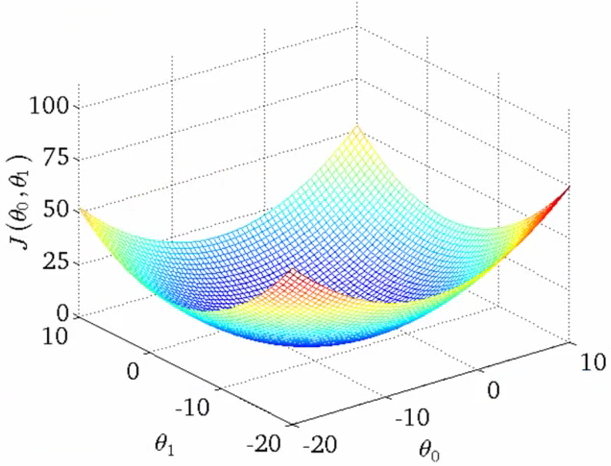
\includegraphics[width=\textwidth]{uni_linreg_j.png}
%%           \caption{An example of \(J(\theta_0, \theta_1)\) from Ng. both moving the th0 and th1 increases quadratically}
%%           \label{fig:unilinreg_a}
%%         \end{subfigure}
%%         \hfill
%%         \begin{subfigure}[b]{0.4\textwidth}
%%           \centering
%%           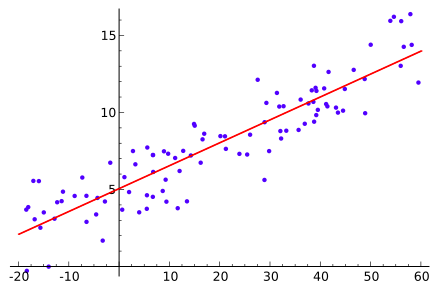
\includegraphics[width=\textwidth]{uni_linreg_h.png}
%%           \caption{an example of \(h(x)\) see how changing th0 (shifting fn) or th1 (gradient) would rise J from wikipedia}
%%           \label{fig:unilinreg_b}
%%         \end{subfigure}
%%         \hfill
%%         \caption{Univariate linear regression: examples for convex \(J\) and optimal \(h\)}
%%         \label{fig:unilinreg}
%%       \end{figure}


\section{Logistic Regression} \label{logreg}

Logistic regression is a classification technique with discrete output. Apart from the fact that classification is required for more complexer tasks, as detection or tracking, logistic regression is especially important in the context of this thesis because it conforms the necessary basis to understand neural networks, as the {\it TensorFlow} API states:
\begin{quote}
  ``The usual method for training a network to perform N-way classification is multinomial logistic regression, aka. softmax regression. Softmax regression applies a softmax nonlinearity to the output of the network and calculates the cross-entropy between the normalized predictions and a 1-hot encoding of the label. For regularization, we also apply the usual weight decay losses to all learned variables. The objective function for the model is the sum of the cross entropy loss and all these weight decay terms, as returned by the loss() function.''\cite{tf-cnn}
\end{quote}

This section will provide a detailed explanation for the multinomial softmax regression, used to classify among \(C\in\mathbb N_{\geq 2}\) different classes, and trained with gradient descent using the cross-entropy as its cost function.

\subsection{Hypothesis for Two-Class Classification}
Any regression model whose hypothesis is based on the \(\theta^T \phi(x)\) dot product can be almost directly used to perform a simple two-class classification: it only needs to be combined with a \textbf{decision boundary}, a real number representing the border between two classes: the positive, labeled as 1 and the negative, labeled with 0. This is achieved by passing the hypothesis to a \textbf{threshold function} (\(Threshold = (\theta^Tx+b)>=t\)), predicting \(x\) as belonging to the \textbf{positive} class when true and \textbf{negative} else, where \(t\in\mathbb{R}\) would be the threshold, usually 0 (again, the identity function \(\phi(x)=x\) is assumed, so it can be omitted until \ref{interaction}). This is the basic idea behind the \textbf{perceptron}\cite[p.729]{russell}, ``the first model that could learn the weights defining the categories given examples of inputs from each category''\cite[p.15]{goodfellow}. A brief and interesting contextualization can be found in the introduction of \cite{vapnik}.\\

But the threshold function has several problems, well summarized in \cite[ch.1]{nielsen} and \cite[p. 725]{russell}: The threshold function is discontinuous, not differentiable and its output announces always a completely confident prediction: 1 or 0. This is problematic for many reasons:
\begin{itemize}
\item Muticlass prediction is not possible: when having more than 2 accepted classes, there is no way to know which one fits best, since all become the same score, a 1.
\item The gradient of the threshold function is always zero except for the boundary, where it is undefined. This makes learning difficult, since it is possible to know if a prediction is false (by comparing it with the label) but not to what extent.
\item Small changes in the hypothesis can produce huge changes in the cost, since all samples that cross the decision border pass from maximal cost to none, or vice versa.
\end{itemize}


\begin{figure}[h]
  \centering
  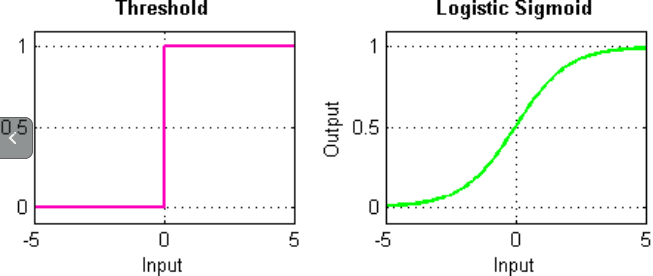
\includegraphics[scale=0.4]{thresh-sig.png}
  \caption{The threshold function with \(t=0\) and the logistic sigmoid\cite{activation-funcs}.}
  \label{fig:sigmoid}
\end{figure}


And there is where logistic regression comes to play: by substituting the threshold function for a softer \textbf{logistic function} (hence the name), all of these issues can be solved to a large extent. For instance, the logistic \textbf{sigmoid} (\(\sigma\)) can be used. It is not as fast to calculate, but it is continuous, differenciable and has a very simple derivative that can be written in terms of its output:

\begin{equation*}
  \sigma(z) = \frac{1}{1+e^{-z}} \qquad \qquad \qquad \frac{d}{dz}\sigma(z) = \sigma(z)(1-\sigma(z))
\end{equation*}\\

This leads to a very efficient calculation, by reusing this output and requiring only one extra subtraction and multiplication. The process of obtaining the derivative will be detailed below.

\begin{tcolorbox}[ams align*]

  The derivative for the sigmoid function can be calculated following the chain rule for derivatives:
  \begin{align*}
    \begin{aligned}
      (f(g(z)))' = f'(g(z))\cdot g'(z)
    \end{aligned}
  \end{align*}
  Where, in the case of \(\sigma(z) = (1+e^{-z})^{-1} = f(g(z))\):
  \begin{align*}
    \begin{aligned}
      & f(z) = z^{-1} \quad \Longrightarrow \quad f'(z) = -z^{-2}\\
      & g(z) = 1+e^{-z} \quad \Longrightarrow \quad g'(z) = -e^{-z}\\
    \end{aligned}
  \end{align*}
  Therefore, it holds:
  \begin{align*}
    \begin{aligned}
      \frac{d}{dz}\sigma(z) = \sigma'(z) &= -(1+e^{-z})^{-2} \cdot -(e^{-z})\\
      & = \frac{e^{-z}}{(1+e^{-z})^{2}}\\
      & = \frac{1}{1+e^{-z}} \cdot \frac{e^{-z}}{1+e^{-z}}\\
      & = \sigma(z) \cdot \frac{1+e^{-z}-1}{1+e^{-z}}\\
      & = \sigma(z) \cdot  \big( \frac{1+e^{-z}}{1+ e^{-z}} - \frac{1}{1+e^{-z}} \big)\\
      & = \sigma(z) \cdot (1 - \sigma(z))\\
    \end{aligned}
  \end{align*}   % ( \big( \Big( \bigg( \Bigg(
\end{tcolorbox}

In the context of neural networks, such functions as the threshold and the sigmoid are called \textbf{activation functions}, because of the analogy to neurons (more on this in section \ref{neuralnetworks}). For a visual comparation between some different activation functions see Figure \ref{fig:sigmoid} .\\


The sigmoid also allows a more refined interpretation: its output can be seen as a probability distribution \(P(y=1|x)\)\cite[p.181]{goodfellow} continuous in the \((0, 1)\) range, and the decision boundary can now be obtained by choosing any \(t\) in such range. The standard is \(t=0.5\), since the probability distribution can be now interpreted as the ``degree of belief'' the system has, being results close to 1 clear positives and results close to 0 clear negatives (note that \(\sigma(z)=0.5\) means that \(z=0\), see \ref{errormetrics} for more information about choosing different values for \(t\)). In this context, the \(z = \theta^Tx\) variable ``defining such a distribution over binary variables is called a \textbf{logit}''\cite[p.182]{goodfellow}.\\

Now it is possible to define the hypothesis for the two-class logistic regression with sigmoid activation function, by \(z\) with \(\theta^Tx\) as the sigmoid's argument:

\begin{equation*}
  h(\theta, x) = \sigma(\theta^Tx) \qquad \qquad \qquad x \text{ is positive} \iff h(\theta, x)>=t\\
\end{equation*}

And last but not least, this hypothesis, combined with the proper cost function, leads to a very efficient formula for the gradient descent algorithm that maximizes the likelihood\cite[p.184]{goodfellow}, with the corresponding nice properties already mentioned in \ref{supervlearning}. This will be explained in detail after describing the multinomial version of the logistic regression, which is a generalization of the two-class model explained so far and shares the same gradient descent formula and likelihood maximization properties.


%% The nice properties of this function apply also when its gradient is used in order to {\it learn} those parameters (see \ref{graddesc} for more details on gradient descent): not only the gradient can be efficiently calculated as already explained, but also it is very adequate: its steepness is maximal in the middle and converges to zero in both extremes. The intuition behind that is that if the sigmoid is interpreted as the ``degree of belief'', the steepness can be seen as the ``permeability to different beliefs'', following the analogy: The more certain the prediction is, the less prone to change will it be. So if gradient descent is initialized in a way that every prediction starts close to the ``center'' (which represents the total uncertainty), the parameters will be able to keep maneuvrability until the predictions converge to one side or the other.\\

%% In this context, the naive approach for a cost function \(J\) would be simply to take the mean square error between each label and the corresponding prediction, as with logistic regression, and then minimize it with gradient descent [QUESTION: IS IT FEASIBLE TO SOLVE IN CLOSED-FORM WITH SIGMOID+MSE?]. This would actually be very problematic, since it would make almost impossible to correct big errors using gradient descent: the gradient of \(J\) for such cases (that is, when \(h\) predicts a value close to 0 but 1 was expected, or vice versa) would be almost zero (see \cite{softmax}), and the model should be able to learn from every failure, especially the big ones.\\

%% So the challenge here is to find a function that avoids this problem, but keeping at the same time the nice properties of the sigmoid: that is exactly what the \textbf{cross-entropy} achieves. But due to the fact that the approach explained so far for two classes is the simplest form of a more general model with \(C\in\mathbb{N}_{\geq2}\) classes, this will be explained in the next subsections in order to avoid duplicity.

\subsection{Hypothesis for Multinomial Classification} \label{multiclass}
Multinomial classification answers the question: ``Having \(C\in\mathbb{N}_{\geq2}\) classes, Which class \(c\in C\) does \(x\) belong to?''. To answer this, it suffices to apply the sigmoid model seen so far multiple times, with a different set of parameters for each class, and picking the answer with the biggest output. But when classifying between disjoint classes (which means the samples can only belong to one class), raising one outcome should obviously reduce the others. The multiple sigmoid approach deprives the model of this knowledge, which is not optimal\cite{softmax}. The \textbf{softmax function} adresses this issue. It ``can be seen as a generalization of the sigmoid function''\cite[p.183]{goodfellow}, and is ``a way of forcing the outputs of \(h\) to sum to 1, so that they can represent the probability distribution across discrete, mutually exclusive alternatives''\cite{softmax}:

\begin{equation*}
  S(z)_c = \frac{e^{z_c}}{\sum_{j=1}^C(e^{z_j})}\\[3mm]
\end{equation*}

In this case, instead of a scalar, this function accepts a \(z\in \mathbb{R}^C\) logit vector and returns a vector of same dimensionality. This output vector behaves also as a probability distribution \(P(y=c | x)\), holding the ``degree of belief'' for each \(z_i\) logit: every output is in the range \((0, 1)\), and the sum of all its outputs is always 1. And, analogous to the sigmoid, its derivative can be also expressed in terms of its output, but the derivation is a little more involved, since it requires some notions on vector calculus. Specifically, the dimension of both output and input components has to be specified:
\begin{equation*}
  \frac{\partial S(z)_a}{\partial z_b} \qquad a,b \in \{1, ..., C\}\\[3mm] %  = S(z)_c(1-S(z)_c)
\end{equation*}

Thus, the complete definition of the derivative comprises \(C\times C\) partial derivatives, which are usually displayed in a matrix called the \textbf{jacobian}\cite[p.86]{goodfellow}. The derivative is explained below.\\

As a side note regarding the properties of the softmax function, dividing the logit vector by a scalar \(\mu\in\mathbb{R}_{>1}\) before passing it to \(S\) will tend to uniformize the output distribution, and multiplying to polarize its belief towards the output with the maximal score. This property can be used to regulate the ``radicality'' of the classificator, which could tend to either equalize or magnify the actual differences. Also, as usual in exponential functions, there are some numerical issues that must have be taken into account, to avoid over- and underflowing when performing their calculation. This is worth to mention, but the present project relies on lower-level libraries to provide a stable implementation and therefore won't be further covered (see \cite[p.81 and p.185]{goodfellow} for more details).


\begin{tcolorbox}[ams align*]

  The jacobian for the softmax function can be calculated following the derivation rule for division:

  \begin{align*}
    \begin{aligned}
      \Big( \frac{f(z)}{g(z)}\Big)' = \frac{f'(z)g(z) - f(z)g'(z)}{g(z)^2}
    \end{aligned}
  \end{align*}
  Where, in the case of \(S(z)_a = \frac{f(z)_a}{g(z)}\):
  \begin{align*}
    \begin{aligned}
      & f(z)_a = e^{z_a} \quad \Longrightarrow \quad \frac{\partial f(z)_a}{\partial z_b}
      = \begin{dcases}
        e^{z_a} = e^{z_b} & \text{if } a=b\\
        0     & \text{otherwise}
      \end{dcases}\\
      & g(z) = \sum_{j=1}^C(e^{z_j}) \quad \Longrightarrow \frac{\partial g(z)}{\partial z_b} = e^{z_b}\\
    \end{aligned}
  \end{align*}
  Therefore, it holds:
  \begin{align*}
    \begin{aligned}
      \frac{\partial S(z)_a}{\partial z_b} = \begin{dcases}
        \frac{e^{z_a}g(z)-e^{z_a}e^{z_b}}{g(z)^2} = \frac{e^{z_a}(g(z)-e^{z_b})}{g(z)g(z)}  = S(z)_a(1-S(z)_a)       & \text{if } a=b\\
        \frac{0g(z)-e^{z_a}e^{z_b}}{g(z)g(z)} = -\frac{e^{z_a}}{g(z)}\frac{e^{z_b}}{g(z)} = -S(z)_a S(z)_b
        & \text{otherwise}
      \end{dcases}\\
    \end{aligned}
  \end{align*}   % ( \big( \Big( \bigg( \Bigg(
  Or, abbreviated:
  \begin{align*}
    \begin{aligned}
      \frac{\partial S(z)_a}{\partial z_b} = S(z)_a(\mathbbm{1}_{i=j}-S(z)_b)
    \end{aligned}
  \end{align*}   % ( \big( \Big( \bigg( \Bigg(
  Where \(a,b\) would also denote the corresponding index in the jacobian matrix.
\end{tcolorbox}


Having this explained, the hypothesis the multinomial version of \(h\) can be now formulated by substituting each \(z_c^{(i)}\) in the softmax function with the actual logit \(\theta_c^Tx^{(i)}\). That means, the model needs \textbf{one \(\theta_c\) parameter vector per class}. In this context, \(h\) can be more generally formulated as follows:\\
\begin{equation*}
  h(\Theta, x)_c = S(\Theta^Tx)_c \qquad \qquad \qquad class(x) = index(max(h(\Theta, x)))\\[3mm]
\end{equation*}
Where \(x\) is still the same feature vector in \(\mathbb{R}^{(n+1)}\) (holding \(n\) features {\it plus the implicit bias}, see \ref{implicitbias}), and \(\Theta\in\mathbb{R}^{(n+1)\times C}\) is a matrix that holds all parameter vectors (one for each class), so the output of \(h\) (as well as the bias term \(b\)) is now a vector with \(C\) dimensions (holding one prediction per class).\\

Especially, note that {\it the one-dimensional version of softmax and its derivative are equal to the two-class model using the sigmoid}. This makes easier to see why this model is a generalization of the former, but there is one notational inconsistency: for \(C\) classes softmax accepts a vector with \(C\) dimensions, whereas for two classes the sigmoid accepts a single scalar instead of a two-dimensional vector.\\

And not only that: a naive implementation of a two-class problem using the general model implementation would require a \((2\times C)\) matrix instead of a \(C\)-dimensional vector, with the corresponding memory and computational overhead. This is worth to note, and should be handled properly when implementing the low-level algorithms, but won't be covered here. Instead, and for convenience reasons, the general notation will be used here for any classification problem with \(C\in \mathbb{N}_{\geq 2}\).\\

It only remains one more inconsistency before finally tackling the cost function and optimization objective for the multinomial logistic regression: the output of the hypothesis for the \(x^{(i)}\) sample is a vector, whereas the predicted label \(class(x^{(i)})\) is a scalar. In this form, a direct comparation between hypothesis and labels is undefined. This is solved by adapting the labels to the so-called \textbf{one-hot} format, explained in the next section.

\subsection{One-Hot Encoding}

As explained before, the output of the hypothesis is a discrete probability distribution in \((0,1)^C\), but the \(y^{(i)}\) labels in the training set are natural numbers in \(\{1, ..., C\}\). In its \textbf{one-hot} version, the natural number \(y^{(i)} = c\in C\) corresponding to the labeled class is converted to a \(\vec{y}\) vector with \(C\) dimensions where all \(\vec{y_i}\) entries are 0 except \(\vec{y_c}\), which is 1:
\begin{equation*}
  y^{(i)}= c  \iff \vec{y}= \begin{bmatrix}y_0 = 0 \\ y_1 = 0 \\ \vdots \\ y_c = 1 \\ \vdots \\ y_C = 0\end{bmatrix}
\end{equation*}
This vector can be now formally compared with the output of \(h\). Note that there are no negative classes in this context, since every one-hot encoded label is positive to exactly one class (a two-class classification would have this way a two-dimensional vector instead of a boolean scalar).



\subsection{Cost Function and Optimization Objective}\label{logregcost}

The cost function used to measure the difference between the hypothesis and the dataset labels is called \textbf{cross-entropy}, designated here with the letter \(\mathcal{L}\) (see \ref{kldivergence} for a more detailed background):

\begin{equation*}
  \mathcal{L}(P, Q) = -\sum_{i=1}^{m} \Big\{P(\epsilon_{ic}) log(Q(\epsilon_{ic})) \Big\}\\[3mm]
\end{equation*}

Whereas the event \(\epsilon_{ic} := \{Y_i=c\}\) corresponds to the \(i^{th}\) sample of some random variable \(Y\) belonging to class \(c\). As we assume that the samples in the dataset are independent and identically distributed (i.i.d), the formula translated to the model explained so far (including the one-hot encoded \(\vec{y}\) labels) turns into:

\begin{equation*}
  J(\Theta, X, y) = -\frac{1}{m}\sum_{i=1}^m \Big\{ log \big(S(\Theta^Tx^{(i)})^T \cdot \vec{y}^{\:(i)} \big) \Big\}\\[3mm]
\end{equation*}


As already anticipated, the optimization of this cost function is equivalent to maximizing the likelihood (with the corresponding consistency and efficiency properties already mentioned in \ref{supervlearning}). Quoting from  \cite[p.184]{goodfellow}:

\begin{quote}
  ``As with the logistic sigmoid, the use of the exp function works very well when training the softmax to output a target value y using maximum log-likelihood [...]. Defining the softmax in terms of exp is natural because the log in the log-likelihood can undo the exp of the softmax''.
\end{quote}


And also importantly, it is very convenient for the optimization with the gradient descent algorithm since its derivative is very efficient to calculate. For instance, note that due to the one-hot encoding, only the \(\vec{y}^{\:(i)}_c = 1\)  component of the label contributes to the dot product with \(S\) (and hence to the cost), so the rest of the components don't have to be calculated. Also, in a {\it i.i.d.} discrete distribution, every sample has a \(P(x^{(i)}) = \frac{1}{m}\), so the term is the same for all of them and can be taken out of the summation. And last but not least, the fact that ``\textbf{the steepness of \(\mathcal{L}\) exactly balances the flatness of \(S\)}''\cite{softmax} allows a great simplification of the derivative, which ends up looking like this (see below for a detailed explanation):

\begin{equation*}
  \frac{\partial}{\partial \Theta}J(\Theta, X, y) = \frac{1}{m}\sum_{i=1}^m \Big\{ (S(\Theta^T x^{\:(i)}) - \vec{y}^{\:(i)}) \cdot x^{\:(i)}^T \Big\} \in \mathbb{R}^{C \times (n+1)}\\[-5mm]
\end{equation*}

This way, the update equation for the gradient descent remains as follows (more information about gradient descent in \ref{graddesc}):


\begin{equation*}
  \begin{aligned}
    \Theta_{next} :&=  \Theta_{current} - \alpha \frac{\partial}{\partial\Theta}J(\Theta_{current}, X, y) \\[3mm]
    &= \Theta_{current} - \frac{\alpha}{m}\sum_{i=1}^m \Big\{ (S(\Theta_{current}^T x^{\:(i)}) - \vec{y}^{\:(i)}) \cdot x^{\:(i)}^T \Big\}\\[3mm]
  \end{aligned}
\end{equation*}

As a side remark, note its great similarity with the gradient descent formula for linear regression.



%% This allows the following reformulation:

%%  \begin{equation*}
%%        J(\Theta, X, y) = -\frac{1}{m}\sum_{i=1}^m \Big\{ log \big(S(\Theta^Tx^{(i)})_{yi}\big) \Big\}\\[3mm]
%%      \end{equation*}

%% With \(S(z)_{yi}\) being the component of the softmax output indexed by the \(y^{(i)} \in \{1, ..., C\}\) label.\\




%% \begin{equation*}
%%      &\frac{\partial}{\partial \Theta_{a,b}} J(\Theta, x^{(i)}, \vec{y}^{\;(i)})  = \begin{dcases}
%%                                     (S(\Theta^Tx^{(i)})-\vec{y}^{\:(i)})x_b^{\:(i)} & \text{if } a=yi\\
%%                                     0  & \text{otherwise}
%%                                     \end{dcases}\\[0mm]
%%      \end{equation*}




\begin{tcolorbox}[ams align*]

  The derivative for the cross-entropy function of the softmax logistic regression (see \cite{softmax} for more references)\\[-20]

  \begin{equation*}
    J(\Theta, X, y) = -\frac{1}{m}\sum_{i=1}^m \Big\{ log \big(S(\Theta^Tx^{(i)})^T \cdot \vec{y}^{\:(i)} \big) \Big\}
  \end{equation*}

  with respect to a parameter \(\Theta_{a,b} \in \mathbb{R}\) (corresponding to class \(a \in \{1, ..., C\}\) and dimension \(b \in \{1, ..., n+1\}\)) can be calculated by applying the multivariate chain rule for multiple nested functions, that is, multiplication of jacobian matrices. But this would yield a very sparse matrix (many entries as it is shown, would be zero), so it can be much more efficiently calculated by treating the functions as univariate derivatives for different cases:

  \begin{equation*}
    % \frac{\partial J}{\partial \Theta_{a,b}} = \frac{\partial J}{\partial S_a}\frac{\partial S_a}{\partial h_a}\frac{\partial h_a}{\partial \Theta_{a,b}}\\[3mm]
    \frac{\partial f(g(h))}{\partial \Theta_{a,b}} = \frac{\partial f}{\partial g} \cdot \frac{\partial g}{\partial h} \cdot \frac{\partial h}{\partial \Theta_{a,b}}\\[1mm]
  \end{equation*}

  This way, the function composition \(f(g(h)) = -log(S(\Theta^Tx^{\:(i)})^T \cdot \vec{y}^{\:(i)})\) represents the cost for the \(i^{th}\) sample, having the following components:
  \begin{align*}
    \begin{aligned}
      &h = \Theta^Tx^{\:(i)} \in \mathbb{R}^C := \text{logit for sample } x^{\:(i)} \in \mathbb{R}^{n+1}\\
      &g = S(z)^T \vec{y}^{\:(i)} = S(z)_c \in (0, 1) := \text{labeled component of the softmax function}\\
      &f= -log(\epsilon) := \text{{\it self-information} of the probability of an event } \epsilon \in [0,1]\\[1mm]
    \end{aligned}
  \end{align*}
  In this context, the partial derivatives of those components are the following:
  \begin{align*}
    \begin{aligned}
      &\frac{\partial h}{\partial \Theta_{a,b}} = \frac{\partial (\Theta^Tx^{\:(i)})}{\partial \Theta_{a,b}}
      % = \frac{\partial (\Theta_{(a,\, ...)}x^{\:(i)})}{\partial \Theta_{a,b}}
      = x^{\:(i)}_b\ \quad \text{(the \(x_{v \neq b}\) components don't interfere)}\\
      &\frac{\partial g}{\partial h} = \frac{\partial S(h)_c}{\partial h} = \begin{dcases}
        S(h)_{c}(1-S(h)_{c}) & \text{if } a=c\\
        S(h)_{c}(0-S(h)_{c})  & \text{otherwise}
      \end{dcases}\\
      &\frac{\partial f}{\partial g}= \frac{\partial(-log(S))}{\partial S} := -\frac{1}{S}\\[-0mm]
    \end{aligned}
  \end{align*}

  See \ref{multiclass} for a detailed derivation of the softmax function. Now it is possible to apply the chain rule to obtain the derivative of the cost for the \(i^{th}\) sample whit respect to the parameter \(\Theta_{a,b}\):\\[-10mm]

  \begin{equation*}
    &\frac{\partial f(g(h))}{\partial \Theta_{a,b}} = \begin{dcases}
      -\frac{1}{S(h)_c} \; S(h)_c(1-S(h)_c) \; x_b^{\:(i)} = (S(h)_c-1)x_b^{\:(i)} & \text{if } a=c\\
      -\frac{1}{S(h)_c} \; S(h)_c(0-S(h)_c) \; x_b^{\:(i)} = (S(h)_c-0)x_b^{\:(i)}  & \text{otherwise}
    \end{dcases}\\[0mm]
  \end{equation*}

  Which very nicely allows to express all the derivatives for the \(\Theta\) matrix at once by using the one-hot encoded label:
  \begin{equation*}
    &\frac{\partial f(g(h))}{\partial \Theta} = \Big( (S(\Theta^T x^{\:(i)}) - \vec{y}^{\:(i)}) \cdot x^{\:(i)}^T \Big) \in \mathbb{R}^{C \times (n+1)}\\[-2mm]
  \end{equation*}
  The derivative for \(J\) over the whole dataset would be then the mean of this derivative for all \(m\) samples.\\[-13mm]
\end{tcolorbox}



\subsection{Final Intuition on Logistic Regression}

Summarizing, logistic regression is a classifying method whose hypothesis function is an affine function that is passed to a logistic layer. The logistic layer allows it to output a degree of confidence for every class, and to learn efficiently from that information.\\

In order to learn, the cross-entropy with softmax can be conveniently used as cost function: not only it is very effective and fast to calculate, but it also ends up being very intuitive: \textbf{the size of the gradient is directly proportional to the size of the error}, which makes it a very natural criterion to correct the difference between labels and hypothesis. This can be clearly seen in the update formula for the gradient descent algorithm.\\

This way, by starting with a very low confidence everywhere (usually \(\Theta\) as a zero matrix, which should cause a numerically stable softmax to output an uniform distribution), the optimization of \(J\) becomes a ``confidence raising process'', in which each labeled example forces the parameters to get away from zero, in order to approximate the response of \(h\) to the corresponding one-hot label: the prediction for the labeled class should get closer to 1, and the rest of predictions to 0. With this process, the model ends up capturing the features that the classes in the dataset may have, since it performs a maximum likelihood estimation. Nevertheless, logistic regression is a linear model and therefore it has its limitations, as it will be discussed in the next section.\\


\section{Non-Linear Hypothesis}\label{interaction}

The linear basis for the logistic regression explained so far, based on the dot product \(\theta^T\phi(x)\), assumes the use of the identity function \(\phi(x)=x\), which results in a linear hypothesis. In that case, the solution provided by the model is a linear combination of linear functions (in the case of the classificators, the boundary of a linear problem is a {\it hyperplane}).  This can be a valid solution for many problems, but many others won't fit into that assumption. For instance, Minsky and Papert demonstrated in 1969 that the linear perceptron cannot solve functions like XOR or NXOR (as explained and exemplified in \cite[p. 10]{deephist}). Moreover, such linear models ``cannot understand the interaction between any two input variables''\cite[p. 169]{goodfellow}.\\

Actually, for many problem domains it is safe to assume that such interactions and non-linear behaviours are present, and, if that is the case, the ability to craft a non-linear hypothesis can lead to a better solution and is desirable. This is done by using a different \(\phi\) function. As explained in \cite[p.169]{goodfellow}, there are three main strategies:
\begin{enumerate}
\item Handcraft \(\phi\). This was the dominant approach until the advent of deep learning. It can be very effective and efficient, but requires high specialization and has little transfer between domains.
\item Choose a very generic \(\phi\) that maps the data to a very high-dimensional space, and work linearly on that space. If the dimensionality is high enough, we can always have enough capacity to fit the training set, but generalization to the test set often remains poor.
\item Let the model itself learn \(\phi\) (the approach of neural networks). This enables the model to capture the benefits of the other approaches, with the drawback that it is the only variant that gives up the convexity.
\end{enumerate}

The implications and details of this approaches will be briefly discussed in the next subsections.


\subsection{Handcrafted Mapping}

By handcrafting the \(\phi(x)\) function to be a polynomial (or equivalent) function it is possible for the hypothesis to capture specific non-linearities and the so-called \textbf{interaction features} without giving up the linearity of the model: it still behaves as a multivariate linear regression, since it is linear respect to the \(\theta\) parameters, and therefore the optimization of \(J\) still works the same as in the linear models explained so far. The following examples help to illustrate how this works:

\begin{itemize}
\item It may be observed that the rent prices in some city grow quadratically when approaching the center. In that case, a polynomial of degree 2 would make appropiate predictions: \(h(\theta, x) = \theta_0+\theta_1x_1+\theta_2x_1^2\). Here, \(h\) has 3 parameters, although the original data has only a single feature (\(x_1\)), representing the distance to the city center.
\item Two different parameters may also interact with each other, like predicting the prize of a car insurance given age (\(x_1\)) and vision capacity (\(x_2\)): the following hypothesis is able to represent even elliptic and hyperbolic curves: \(h(\theta, x) = \theta_0+\theta_1x_1+\theta_2x_2+\theta_3x_1x_2+\theta_4x_1^2+\theta_5x_2^2\).
\end{itemize}

The intuition behind this examples is the following:  both \textbf{embed} the data into a higher dimensional space, in which they find a linear hypothesis that will reflect the ground truth more closely, or, at least, perform as good as a linear hypothesis (by optimizing the non-linear \(\theta\) coefficients to zero). In fact:
\begin{quote}
  ``\textbf{If the data samples are mapped into a space of sufficiently high dimension, then they will be almost always linearly separable} ---if you look at a set of points from enough directions, you'll find a way to make them line up [...] four dimensions suffice for linearly separating a circle anywhere in the plane (not just at the origin), and five dimensions suffice to linearly separate any ellipse. In general (with some special cases excepted) if we have \(N\) data points then they will always be separable in spaces of \(N-1\) dimensions or more''\cite[p. 746]{russell}.
\end{quote}

\begin{figure}
  \centering
  \begin{subfigure}[b]{0.36\textwidth}
    \centering
    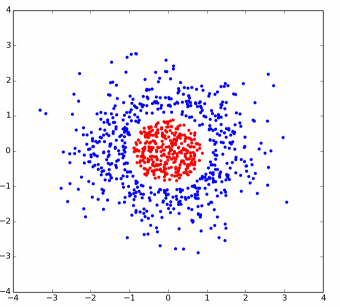
\includegraphics[width=\textwidth]{interact-ft1.png}
    \caption{original 2D dataset}
    %\label{}
  \end{subfigure}
  \hfill
  \begin{subfigure}[b]{0.5\textwidth}
    \centering
    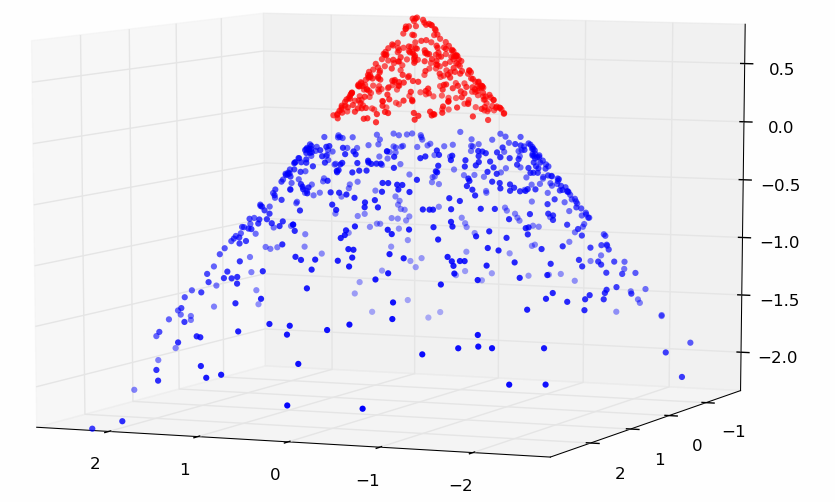
\includegraphics[width=\textwidth]{interact-ft2.png}
    \caption{dataset embedded to a 3^{rd} dimension\\\(\;z = 1-\sqrt{x^2 + y^2}\) becomes linearly separable at \(z=0\)}
    %\label{}
  \end{subfigure}
  \hfill
  \caption{http://stackoverflow.com/questions/1148513/difference-between-a-linear-problem-and-a-non-linear-problem-essence-of-dot-pro}
  \label{fig:interact}
\end{figure}

See figure \ref{fig:interact} to complete this intuition with an example of a classification problem. As a side remark regarding the use of a polynomial \(\phi\), note that it can be desirable to apply mean normalization when optimizing with gradient descent, since the ranges of the features grow very fast when multiplied/exponentiated, and this can delay or even skew the convergence of the algorithm. Actually, and depending on the used software, even optimizing with the normal equations may also benefit from to normalizing the data to avoid error propagation (see {\it poor conditioning}, \cite[p.82]{goodfellow} for more information).\\


\subsection{Generic Mapping}

Ideally, \(\phi\) is handcrafted to provide the smallest embedding possible to effectively model the data. But note that the number of parameter combinations grows exponentially with the number of dimensions, so choosing by hand which combination fits best can become a very time-consuming and is reasonable only in a small scale.Rather,  the \textbf{kernel trick} can be used. Quoting \cite[p.141]{goodfellow}, it ``consists of observing that many machine learning algorithms can be written exclusively in terms of dot products between examples''. For instance, it can be shown that

\begin{equation*}
  \begin{aligned}
    \theta^T\phi(x) = \sum_i^m \{ \alpha_i \phi(x)^T\phi(x^{(i)})\}
  \end{aligned}
\end{equation*}

Where \(x\) is the current input, \((x^{(1)}, ..., x^{(m)})\) the training examples and \(\alpha\) a vector of coefficients. Quoting further,
\begin{quote}
  ``Rewriting the learning algorithm this way allows us to replace x by the output of a given feature function \(\phi(x)\) and the dot product with a function \(k(x, x^{(i)}) = \phi(x)^T\phi(x^{(i)})\) called a kernel [...]. The kernel trick is powerful for two reasons. First, it allows us to learn models that are nonlinear as a function of x using convex optimization techniques that are guaranteed to converge efficiently. This is possible because the optimization algorithm can view the decision function as being linear in a different space. Second, the kernel function k often admits an implementation that is significantly more computational efficient than naively constructing two \(\phi(x)\) vectors and explicitly taking their dot product.In some cases, it can even be infinite dimensional (using, for example, the \textbf{RBF} kernel function), which would result in an infinite computational cost for the naive, explicit approach [...]. The category of algorithms that employ the kernel trick is known as \textbf{kernel machines} or \textbf{kernel methods}''.\cite[p.141]{goodfellow}
\end{quote}

Because of this nice properties, kernel machines, like like the {\it Support Vector Machines}, are a very reasonable off-the-shelf model for many problem domains. But they also present disadvantages. One of them, already anticipated, is that they often lack generalization ability. Also, they don't scalate well for big datasets: the evaluation of the hypothesis function is linear to the number of samples, and:

\begin{quote}
  ``Prior to the advent of deep learning, the main way to learn nonlinear models was to use the kernel trick in combination with a linear model. Many kernel learning algorithms require constructing an \(m\times m\) matrix \(G_{i,j} = k(x^{(i)},x^{(j)})\). Constructing this matrix has computational cost $\mathcal{O}(n^2)$, which is clearly undesirable for big datasets. In academia, starting in 2006, deep learning was initially interesting because it was able to generalize to new examples better than competing algorithms when trained on medium-sized datasets with tens of thousands of examples. Soon after, deep learning garnered additional interest in industry, because it provided a scalable way of training nonlinear models on large datasets.''\cite[p.152]{goodfellow}
\end{quote}

For this reasons, kernel machines weren't used in the context of this thesis and therefore won't be further covered.


\section{Neural Networks}\label{neuralnetworks}

Neural networks can be thought as a stack of linear classifiers on the top of each other, interleaved with some activation layer to avoid the so-called {\it linear lasagna} (since a linear combination of linear layers is equivalent to a single linear layer).\\

See Figure \ref{fig:neurons} for an illustration of the natural and artificial models for a neuron. This basic concept allows a great flexibility: the approaches explained so far have an explicit separation between designing the model and training it on the data. This is the main difference with neural networks: instead of directly mapping the data to a certain space, this models perform multiple mappings, which are learned during the training: the initial one becomes the data, and the last one outputs the classification; but the intermediate ones are learned by the model.\\

This can be put under the broad category of \textbf{representation learning}: ``the last layer of the network is typically a linear classifier, such as a softmax regression classifier. The rest of the network learns to provide a representation to this classifier. Training with a supervised criterion naturally leads to the representation at every hidden layer (but more so near the top hidden layer) taking on properties that make the classification task easier. For example, classes that were not linearly separable in the input features may become linearly separable in the last hidden layer''\cite[p.530]{goodfellow}. There are many ways to implement this idea. In fact, the great flexibility that NN-related models show is one of their strengths, since it makes easier to compromise between hand-engineeried parts and end-to-end training.\\

But this flexibility has also a drawback: the more abstraction is managed by the model, the harder can become for us to interpret what is happening and why is working. This empirical approach is known as \textbf{end-to-end}, because the setup only has explicit control over both the input and the output.\\

The main way of classifying neural networks is by the linear operation that they perform in their layers. If the operation is a matrix-multiplication, that layer is said to be a fully conected, because the matrix contains a weight for every single row-to-column pair, representing the connections between every column-neuron to every row-neuron. The other main type of linear operation, relevant for this thesis, is the convolution. As explained in \cite[p.176]{goodfellow} ``Designing and training a neural network is not much different from training any other machine learning model with gradient descent''. In fact, the only main difference and one of the main reasons of the success of neural networks is the application of the \textbf{backpropagation} algorithm, which leverages the application of the chain rule for specific families of functions in order to compute the derivatives across the layers of the neural network very efficiently. See \cite[p.203]{goodfellow} for a detailled explanation on backpropagation for the different families of neural networks.\\

Another important factor involving the definition of a neural network is the activation function used. ``In modern neural networks, the default recommendation is to use the ReLU''\cite[p.173]{goodfellow}. ReLU is an acronym for Rectified Linear Unit, which in its basic form is the function \(f(x) = max(0, x)\). Its simplicity gets reflected in the numerical stability and computational simplicity of its derivative, which makes it very suitable for ``modern'' networks, which usually feature more layers and representational power. The other prominent activation function, the sigmoid/softmax family, has already been explained in section \ref{logreg}.\\

\begin{figure}
  \centering
  \begin{subfigure}[b]{0.35\textwidth}
    \centering
    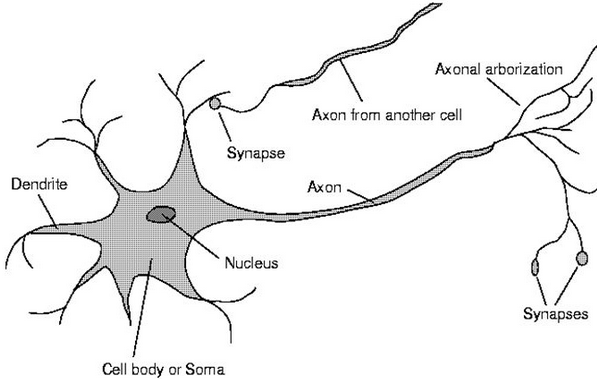
\includegraphics[width=\textwidth]{neuron.png}
    \caption{``The parts of a nerve cell or neuron'', from \cite[p.11]{russell}}
    \label{fig:neuron}
  \end{subfigure}
  \hfill
  \begin{subfigure}[b]{0.6\textwidth}
    \centering
    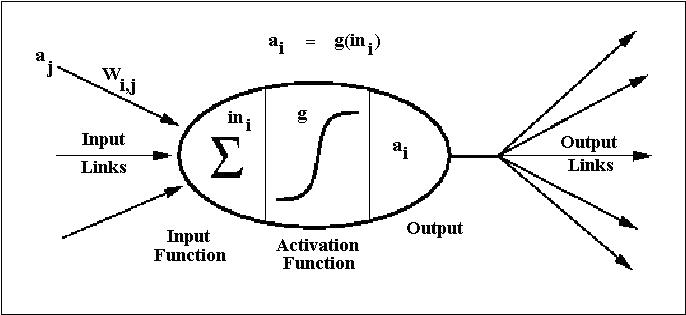
\includegraphics[width=\textwidth]{neuron-model.png}
    \caption{``A simple mathematical model for a neuron'', from \cite[p.728]{russell}}
    \label{fig:neuron-model}
  \end{subfigure}
  \hfill
  \caption{``One should not view deep learning as an attempt to simulate the brain [...]: it is primarily concerned with how to build computer systems that are able to successfully solve tasks requiring intelligence, while the field of computational neuroscience is primarily concerned with building more accurate models of how the brain actually works.''\cite[p.17]{goodfellow}}
  \label{fig:neurons}
\end{figure}


\subsection{Convolutional Networks}

\subsubsection{Parameter Sharing}

Fully connected layers have a great representational power, but it has been shown that deeper networks with smaller layers are more meaningful and perform empirically better\cite[p.202]{goodfellow}. One key concept in this context is the idea of parameter sharing, ``a way to express our prior knowledge about suitable values of the model parameters, by, for instance, forcing sets of parameters to be equal''\cite[p.251]{goodfellow}. This has been proven especially helpful with convolutional networks, which naturally capture such prior knowledge as locality.\\

\subsubsection{Convolution and Pooling}

As every neural network, CNNs consists of multiple layers. And within each layer, we typically find ``three stages. In the first stage, the layer performs several convolutions in parallel to produce a set of linear activations. In the second stage, each linear activation is run through a nonlinear activation function, such as the rectified linear activation function. This stage is sometimes called the detector stage. In the third stage, we use a pooling function to modify the output of the layer further''\cite[p.340]{goodfellow}.\\

The convolution, is a linear operation that, somewhat like the dot product, acts like an ``affinity filter'' between two functions. In fact, convolution is equivalent to performing many localized dot products between that two functions (one of them reversed), giving thus a ``by-position'' affinity between those two functions. In the case of the neural networks, one of those functions is the data and the other is the so-called ``kernel''. See \cite[p.332]{goodfellow} for a more detailled explanation. For this reason, the size of the kernel is an important factor: for a specific location, it will determine the range of the data that will be regarded to compute that dot product. \\

Pooling is the other major operation involved in convolutional neural networks: it ``replaces the output of the net at a certain location with a summary statistic of the nearby outputs''. For example, ``the max pooling operation reports the maximum output within a rectangular neighborhood''\cite[p.340]{goodfellow}. Pooling introduces a strong prior into the architecture: the locality, in other words, the idea that the dot products returned by the convolution that are close to each other are related.\\

\subsubsection{Architecture}

Usually, each convolutional layer contains several kernels, in order to capture the different independent features that the data may show. The number of kernels determines the number of channels of the outcoming representation, also known as its ``depth''.\\

A typical approach for a convolutional neural network is to increase the depth layer by layer, and decrease the width and heigth via the pooling operation, until reaching a representation of just one pixel but arbitrary depth. This to-be-learned representation is then passed to a classifier placed on the top of the network, which outputs then the logits.

%% http://stats.stackexchange.com/questions/182734/what-is-the-difference-between-a-neural-network-and-a-deep-neural-network?rq=1
%% http://neuralnetworksanddeeplearning.com/chap5.html


\section{General Concepts} \label{general-concepts}

\subsection{Implicit Bias Notation}\label{implicitbias}

In linear classification models, the calculation of the {\it logits} corresponds to an \textbf{affine function}, that is, a linear transformation followed by a translation. This translation is necessary to approximate functions with constant components, and is achieved by adding a \textbf{intercept} or \textbf{bias term} \(b\) to the dot product:\\
\begin{equation*}
  h(\theta, b, x) = \theta^Tx+b
\end{equation*}

This single bias term has to be learned exactly the same way as any other parameter; in fact, it {\it is} an extra parameter. Based on this observation, the formula above can be expressed in a more compact way: prepending the terms \(\theta'_0=b\) and \(x'_0=1\) to the \(\theta'\) and \(x'\) vectors leaves the following equivalent expression
\begin{equation*}
  h(\theta', x') = \theta'^{\,T}x'
\end{equation*}

The quote in \(\theta'\) and \(x'\) is to note that they have {\it one more dimension} than their corresponding counterparts, that is, \(n+1\) dimensions: the \(n\) features plus the implicit bias \(\theta'_0*x'_o=b*1=b\), incorporated as the ``zero-dimension'' or feature. The equivalence \(\theta^Tx+b= \theta'^{\,T}x'\) becomes then evident. Unless specified otherwise, the dot product with implicit bias will be the default notation in this thesis, so for convenience it will be expressed without the quotation mark (that is, \(\theta^Tx\)).

\subsection{Gradient Descent}\label{graddesc}
Gradient descent\cite{cauchy} is a family of algorithms that perform numerical optimization of functions, that is, finding a value for \(x\) that minimizes (or maximizes) \(y=f(x)\). They come to use for non-linear models (like neural networks), where ``most cost functions can no longer be optimized in closed form. This requires us to choose an iterative numerical optimization procedure, such as gradient descent''\cite[p.153]{goodfellow}. In fact, some models may even ``require special-case optimizers because their cost functions have flat regions that make them inappropriate for minimization by gradient-based optimizers''\cite[p.154]{goodfellow}.\\

In general, non-convex optimization can be a very complex domain way beyond the scope of this thesis, so, following the global trend, it will be assumed here that many models (including neural networks) ``work very well when trained with gradient descent''\cite[p. 152]{goodfellow}, since  ``it often finds a very low value of the cost function quickly enough to be useful''\cite[p. 152]{goodfellow}.

\subsubsection{Intuition Behind Gradient Descent}
The gradient of a function \(y=f(x)\) is useful for minimizing \(f\), because ``it tells us how to change \(x\) in order to make a small improvement in \(y\)'' (see \cite[p. 83]{goodfellow} for more details). This is the basic idea behind gradient descent: starting from a given \(x\), it is possible to iteratively ``reduce \(f(x)\) by moving \(x\) in \textbf{small steps} with opposite sign of the derivative of \(f\)''\cite[p. 83]{goodfellow}, until it converges to a point with zero gradient (see the next subsection for the mathematical formulation). This point is ideally the global minimum of the function, but it also can be any local minimum, a saddle point or even a maximum.\\

More precisely, when having a cost function \(J(\theta, X)\) that states how well an hypothesis performs for the given dataset \(X\), its partial derivatives on the \(\theta\) parameters will tell us how to (locally) change \(\theta\) in order to reduce the overall cost. Figure \ref{fig:graddesc} may also help to become a very basic intuition: the process closely resembles the idea of ``dropping a ball'' at any starting point and letting it fall down the direction of the slope, having a ``speed'' proportional to the steepness.\\

\begin{figure}[h]
  %\hspace*{-0.6cm}
  \centering
  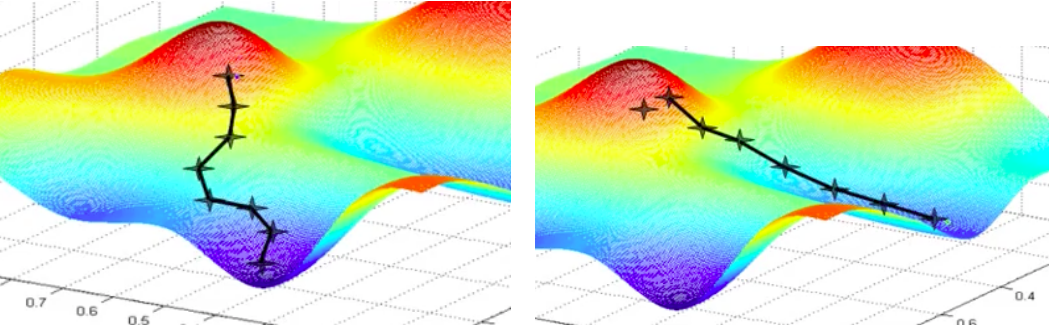
\includegraphics[scale=0.4]{graddesc.png}
  \caption{Two different gradient descent optimizations of the same non-convex function: the slightly different starting points lead to different local minima (from \cite{coursera-ml} video: ``Gradient Descent'').}
  \label{fig:graddesc}
\end{figure}

The explanation so far comprises the intuition behind the ``vanilla'' version of the algorithm, the \textbf{batch gradient descent} (abbreviated {\it BGD}), which is presented in the next subsection. This basic version is exposed to many issues that can drastically alter its performance, and for most complex settings requires some tweaking to be able to perform acceptably. In fact, the different algorithms of the gradient descent family are variations of the {\it BGD} motivated by such issues. Therefore it is desirable to have a sound understanding of the {\it BGD}, in order to be able to identify possible performance issues, understand their cause and identify the most appropiate variation for each case. This will also be covered in the next subsections with some detail.\\

\subsubsection{Batch Gradient Descent}

The general strategy is to start with any convenient parameter vector \(\theta^{(0)}\) and {\it simultaneously} update all its \(\theta_j\) components as follows:
\begin{equation*}
  \begin{aligned}
    & \text{repeat until \(|\theta_j^{\,(i+1)}-\theta_j^{\,(i)}|<\epsilon\):}\\[5mm]
    & \qquad \qquad \theta_j^{\,(i+1)} :=  \theta_j^{\,(i)}-\alpha\frac{\partial J}{\partial\theta^{\,(i)}_j}  \\[3mm]
    & i \in \mathbb{N}, \quad \epsilon, \alpha \in \mathbb{R}^+, \quad \theta  \in \mathbb{R}^{(n)}, \quad  \forall j \in \{1, ...,  n\}
  \end{aligned}
\end{equation*}

\(|\theta_j^{\,(i+1)}-\theta_j^{\,(i)}|<\epsilon\) is the convergence condition: Ideally, it would be sensible to say ``repeat until convergence'' instead, which would imply that \(\epsilon=0\), but in some cases, it may be convenient to stop before this happens. In others, it may be desirable to keep going.\\

The \(\alpha\) factor is called the \textbf{learning rate}, and affects directly the size of each step. As already seen, for non-convex functions the information given by the derivative holds only locally. More precisely, holds only at infinitesimal level: this means that the most precise way to update \(\theta\) would be to have the smallest \(\alpha\) possible, but this would maximize the number of iterations needed in order to converge. On the opposite side, a very big \(\alpha\) would cause the algorithm to go ``too far away'', and the information given by the derivative of \(J\) would become useless (in some cases an oversized learning rate could even make {\it BGD} diverge to the infinity). So in an ideal scenario, it would be possible to apply the optimal \(\alpha\) to each iterative step, but due to the properties of most const functions, there is no trivial systematic way of calculating it. In fact, choosing the appropiate learning rate is one of the key points which the different gradient descent variants focus on.\\

%% Luckily enough, it is possible to know if it is too small or too big (NG VIDEOS ON EVOLUTION CURVES WHEN m PROGRESSES?). It must also be noted that, even with a fixed learning rate, the size of steps will decrease if the gradient itself will become smaller. This can mean, with some luck, that the step size will nicely adapt when converging to a minimum, but could also make some parameters converge into any suboptimal zero-gradient point (e.g. bad local minima, \textbf{local maxima} or \textbf{saddle points}), and stop there. It is possible to overcome, or at least mitigate some of this issues by applying MOMENTUM to the vector, and SECOND, THIRD ORDER?? (hessian, jacobian) derivatives. Other gradient descent variations explained here will as well focus on this techniques.\\
%% regarding momentum: \url{http://distill.pub/2017/momentum/}

And last but definitely not least, there is a performance problem: every cost function, as well as any of its derivatives, is based on a given dataset, and requires to perform calculations for every given sample. On the top of that, BGD does this for every feature, once per iteration! (hence the ``batch'' term). So given m samples, j features and i total steps until convergence, the worst-case amount of operations will be BGD=O(m*j*i), which scalates very poorly. There are GD variations that overcome this problem, as explained further on. (vectorization, parallel GD, SGD, miniBatchGD, early stopping)\\



\subsubsection{Stochastic and Minibatch Gradient Descent}

``Stochastic gradient descent has many important uses outside the context of deep learning. It is the main way to train large linear models on very large datasets. For a fixed model size, the cost per SGD update does not depend on the training set size m. In practice, we often use a larger model as the training set size increases, but we are not forced to do so. The number of updates required to reach convergence usually increases with training set size. However, as m approaches infinity, the model will eventually converge to its best possible test error before SGD has sampled every example in the training set. Increasing m further will not extend the amount of training time needed to reach the model’s best possible test error. From this point of view, one can argue that the asymptotic cost of training a model with SGD is O(1) as a function of m''\cite[p.152]{goodfellow}

Again, starting with any convenient parameter vector \(\theta^{(0)}\) and {\it simultaneously} updating all its \(\theta_j\) components:
\begin{equation*}
  \begin{aligned}
    & m \in \mathbb{N}\;\hat{=} \text{ dataset size}\\
    & b \in \mathbb{N}\;\hat{=} \text{ batch size, } b\leq m\\
    & I \in \mathbb{N}\;\hat{=} \text{ number of iterations}\\[5mm]
    & \text{1) shuffle all } (X^{(i)}, y^{(i)}) \text{ tuples in the dataset}\\[2mm]
    & \text{2) for } i \in \{1, ..., I\} \text{:}\\[5mm]
    & \qquad \qquad j := (b*i)(mod\;m)\\
    & \qquad \qquad \theta^{\,(i+1)} :=  \theta^{\,(i)}-\frac{\alpha}{b}\frac{\partial}{\partial\theta^{\,(i)}}J(\theta, X^{(j...(j+b))}, y^{(j...(j+b))})  \\[3mm]
    & \alpha \in \mathbb{R}^+, \quad \theta  \in \mathbb{R}^{(n)}, \quad  \forall j \in \{1, ...,  n\}
  \end{aligned}
\end{equation*}


\subsubsection{Further Optimizations}

One of the problems that poses the use of gradient descent, is the application of a proper learning rate. This issue becomes even bigger in the stochastic gradient descent algorithm, which features also further hyperparameters like the batch size. Algorithms like the Adam optimizer\cite{adam} offer a solution to this problem by taking into account further derivatives of the cost function (the so-called Hessian and Jacobian matrices) in order to calculate a dynamic, context-depending learning rate.



%%    \subsection{Overfitting and Regularization}\label{regularization}

%% http://neuralnetworksanddeeplearning.com/chap3.html

%%   reminder: the derivative of L2 \(\lambda* 0.5 * \Theta\) with respect to theta a,b is lambda* theta a,b

%%    FIGURES:
%%    in log.reg., comparative graph showing effects of regularization: no reg, ok reg, high reg



%%    When a model tends to oversimplify his hypothesis, we say it is \textbf{biased}. And conversely, if due to its excesive capacity tends to memorize the training data thus failing to generalize, we say it is \textbf{overfitting} the data. A more intuitive vision is given by the {\it skinny jeans} approach\cite{stretchpants}: finding the model that fits perfectly (the skinny jeans) is very hard, so everybody end up wearing loose pants (overfitting). The solution for that are the stretchpants (regularizing): ``they fit well, but because they're flexible, they don't make things harder to fit in''. Thus, \textbf{``regularizing means applying artificial constraints on your network, that implicitly reduce the number of free parameters, while not making it more difficult to optimize''}.

%%    -early termination still the best way

%%    In his
%%    l2 and dropout regul. overfitting and bias

%%    normal equations:  (see \url{https://en.wikipedia.org/wiki/Regularization_(mathematics)#Tikhonov_regularized_least_squares}).

%%    \subsection{Cross Validation}\label{crossvalidation}
%%    FIGURES: learning curves for bias, overfitting and ok
%%    In supervised learning, the problem formulation talks about a training set. Apart from the considerations in\ref{datapreprocessing}, the bigger it is, better for the system
%%    cross validation set, learning curves

%%    higher-order CV procedures: auto-weka (2016): \url{http://www.cs.ubc.ca/labs/beta/Projects/autoweka/}
%%    \subsection{Error Metrics}\label{errormetrics}
%%    precision recall f2
%%    en logreg,hablar de cambiar el threshold para variar el prec y recall

%% voting


%%         TALK ABOUT AUC ROC?



\subsection{KL-Divergence and Cross-Entropy}\label{kldivergence}

The cross-entropy is used to measure the similarity between the hypothesis and the dataset in classification problems, modelled as probability distributions. To become a better idea on how does this work, some background on information theory is needed. Specifically, how to quantify the information given by a probability distribution. Most of the explanations of this section (especially the quotes), as well as extra information can be found in \cite[p.73]{goodfellow}.
\subsubsection{Self-Information and Shannon entropy}

The information of an event \(\epsilon_{ic} := \{Y_i=c\}\) given by any probability distribution \(P(Y)\) is related, among other things described in \cite[p.73]{goodfellow}, to the likelihood of that event: ``learning that an unlikely event has occurred is more informative than learning that a likely event has occurred''. It can be quantified with the {\it self-information} of such event:
\begin{equation*}
  I(\epsilon_{ic}) = -log(P(\epsilon_{ic}))\\[3mm]
\end{equation*}
If the basis of the logarithm is 2, the returned value is the amount of information in {\it bits}. If the natural logarithm (with basis \(e\)) is used, the information unity are the {\it nats}: ``One nat is the amount of information gained by observing an event of probability \(e^{-1}\)''\cite[p.73]{goodfellow}. This way it is also possible to quantify the average amount of information in the whole distribution by calculating the expectation for the self-information over all its possible outcomes. This is known as the {\it Shannon entropy} of the variable, expressed here in its version for discrete probability distributions:
\begin{equation*}
  H(P) = \mathbb{E}_P[I(Y)] =  \sum_{i=1}^{m} \Big\{P(\epsilon_{ic}) I(\epsilon_{ic}) \Big\} =  - \sum_{i=1}^{m} \Big\{P(\epsilon_{ic}) log(P(\epsilon_{ic})) \Big\}\\[3mm]
\end{equation*}

When used with basis 2, this calculation ``gives a lower bound on the number of bits needed on average to encode symbols drawn from a distribution \(P\). Distributions that are nearly deterministic (where the outcome is nearly certain) have low entropy; distributions that are closer to uniform have high entropy''.

\subsubsection{KL-Divergence}
``If we have two separate probability distributions \(P(Y)\) and \(Q(Y)\) over the same random variable Y, we can measure how different these two distributions are using the Kullback-Leibler (KL) divergence'':
\begin{equation*}
  D_{KL}(P || Q) = \mathbb{E}_P[log(P(Y))-log(Q(Y))] = \sum_{i=1}^{m} \Big\{P(\epsilon_{ic}) (log(P(\epsilon_{ic}))-log(Q(\epsilon_{ic})) \Big\}\\[3mm]
\end{equation*}

The KL-divergence is non-negative, and zero if and only if both distributions are identical. For this reason ``it is often conceptualized as measuring some sort of distance between these distributions. However, it is not a true distance measure because it is not symmetric''. There are some caveats (especially the fact that it is not a symmetric operation, and others explained in \cite[p.74]{goodfellow}), but the idea of measuring the distance between two distributions will suffice for the present explanation.

\subsubsection{Cross-Entropy and Intuition}
When training a classificator, the information of the dataset as a probabiliy distribution can be purely regarded in terms of the information contained in its labels. Conversely, the hypothesis of the model can be also regarded as a different distribution, generating a different set of labels. This way, the KL-Divergence can be systematically used to measure how well does the hypothesis resemble the training data, regardless of the specific features of the data space. In that case, the optimization objective is to minimize it, which can be done with gradient descent. This is precisely the strategy followed by unsupervised learning algorithms like t-SNE\cite{t-sne}.\\

But, when performing supervised learning, only the distribution given by the hypothesis is optimized, so it is not necessary to take both \(log(P(Y))\) and \(log(Q(Y))\) terms into account. This is where the cross-entropy comes into play:

\begin{equation*}
  \mathcal{L}(P, Q) = -\mathbb{E}_P[log(Q(Y))] = -\sum_{i=1}^{m} \Big\{P(\epsilon_{ic}) log(Q(\epsilon_{ic})) \Big\}\\[3mm]
\end{equation*}

In other words, ``minimizing the cross-entropy with respect to Q is equivalent to minimizing the KL divergence, because Q does not participate in the omitted term''\cite[p.75]{goodfellow}. An explanation on how to use it in combination with the softmax function to perform gradient descent optimization can be found in \ref{logregcost}.

%% \subsection{Robust Models}\label{robust}

%%       Applying the same cost function to every sample and taking the overall average causes the model to be sensitive to noisy and context-dependent data. For example, hardware errors and other excepcionalities may generate samples way out from the context, greatly incrementing the output of the cost function, thus affecting the learning process. Robust regression methods (as, for example, the {\it Theil-Sen estimator}, see \cite{theil} and \cite{sen}) incorporate extra criteria to define a \textbf{prior} context in which data is expected to happen, and properly handle such cases in which out-of-context samples, known as \textbf{outliers} may skew the result. As for 2017, wikipedia warns\cite{robust-wiki} that such methods are surprisingly unpopular:

%% \begin{quote}
%% Despite their superior performance over least squares estimation in many situations, robust methods for regression are still not widely used. Several reasons may help explain their unpopularity (Hampel et al. 1986, 2005). One possible reason is that there are several competing methods and the field got off to many false starts. Also, computation of robust estimates is much more computationally intensive than least squares estimation; in recent years however, this objection has become less relevant as computing power has increased greatly. Another reason may be that some popular statistical software packages failed to implement the methods (Stromberg, 2004). The belief of many statisticians that classical methods are robust may be another reason.
%% \end{quote}

%% And indeed, the fact that such ``bibles'' as \cite{russell}, \cite{bishop} or \cite{goodfellow} do not contain a single reference to the term is a strong indicator of that. Regarding this thesis, as already explained in the beginning of this chapter, it is assumed that the dataset is comprehensive and correctly labeled and therefore no robust methods will be needed. For this reason, they won't be further covered (see \cite{andersen} and \cite{tendeiro} for a broad coverage on the topic).


%% \subsection{Non-parametric Models}\label{nonparametric}

%%                            REVISE THIS! quote ``all of statistics'' for definition of NPM. Also talk briefly about KNN (see goodfellow p. 143) because the 2015 paper uses it. \cite{svm_knn}

%%         All the models explained so far are parametric, meaning that they have a fixed set of parameters independently of how does the data look like. This forces the model to make some assumptions on the data and its context, which has advantages and disadvantages. Non-parametric models adapt their architecture to the given dataset, which implies a totally different workflow, in which the data itself directly influences many design decisions. For this reason, this approach is known as {\it data-driven} design (as opposed to the {\it model-driven} approach associated with parametric models).\\
%%         Both approaches are legitimate and useful depending on the context. Currently, parametric models are gathering the most attention. The reasons for that are that, in the best-case scenario,  having a fixed set of parameters and their combinations can lead to an explicit interpretation on how does the ``ground truth'' work, which can help to transfer the achieved knowledge to other domains and applications more easily. Plus, because of their more predictable architecture, it is possible to achieve a better sinergy amongst the different components (especially libraries and hardware) and effectively scale them up.\\
%%         Of course, the best-case scenario for parametric models doesn't always apply, and some problem domains can be tackled more effectively following a {\it data-driven} approach. Non-parametric models are in any case a field of expertise on their own and won't be covered here since they didn't play a relevant role in this thesis. Some examples of non-parametric models are: {\it pieceweise linear nonparametric regression} (a.k.a. ``connect-the-dots''), {\it \(k\)-nearest neighbours average}, {\it \(k\)-nearest neighbours regression} and {\it locally weighted regression}.

%% \subsection{Universal Approximation Theorem}
%% asdf

%% %% \subsection{Central Limit Theorem?}
%% %% asdf

%% %% \subsection{Manifolds}
%% %% fdas

%% \subsection{Invariance}
%% fdas

%% \subsection{Sparsity and Parameter Sharing}
%% \url{http://ml.typepad.com/machine_learning_thoughts/2005/11/when_does_spars.html}


\chapter{About the Implementation}\label{implementation}
In order to describe the experiments that I've conducted in the context of this thesis, two general aspects have to be covered: one, common for all the experiments conducted, concerns the tools that I used, as well as the specific pipeline that I developed, in order to be able to conduct such experiments. This will be the focus of the present chapter.\\
The other aspect, specific for each experiment, concerns the motivations that led to every specific experiment, together with a description of the settings, architectures and results involved, as well as the interpretation of the results that led to subsequent experiments. This will be discussed in chapter \ref{experiments}.\\

Note that the following general considerations apply to the whole chapter:
\begin{itemize}
\item All the Python scripts can be found under the https://github.com/andres-fr/bachelor-thesis/code/ link.
\item The data and the labels can be found under the https://github.com/andres-fr/bachelor-thesis/datasets/ link.
\item The computer language used for the development of the whole project is \texttt{Python 2.7}.
\end{itemize}



\section{Data Downloading and Storage}

As described in chapter \ref{about-ds}, the curators of the carnatic corpus developed and kindly granted us access to Dunya, an open-source platform that provides a web service as well as a Python API for accessing the labels and recordings needed to conduct the experiments. The source files, together with a description of their usage can be found in the following GitHub link: \url{https://github.com/MTG/dunya}.\\

The API function \texttt{get\_recordings()} provides a list of unique IDs, that can be used to access each recording as an mp3 file, and its label as a dictionary of unicode strings. See the Python scripts \texttt{1\_download\_carnatic.py} and \texttt{2\_download\_metadata\\.py} in the \texttt{code} folder for more details.\\

The downloaded data is stored as \texttt{HDF5} (a binary data format that allows storage of huge amounts of numerical data), via the \texttt{h5py} Python package\cite{h5py}, which is allows to ``easily manipulate HDF5 data from NumPy''\cite{h5py}. \texttt{NumPy} is ``the fundamental package for scientific computing with Python''\cite{numpy}.\\

HDF5 alows different ranges of lossless compression on the stored data, as well as very flexible hashing and indexing of the data chunks. In the Python implementation, it is organized in the form of dictionaries in which the keys are strings and the data are NumPy arrays. The keys can then be grouped into higher-order dictionaries, allowing the creation of tree structures.\\

For a single-label, supervised classification task, this way of organizing the data makes the idea a dictionary of dictionaries (here abbreviated as {\it ddict}) a very natural way to store and structure the downloaded datasets: the higher-ordered dictionary stores the label (in our case the r\=aga's ID) as a key and the lower-ordered dictionary as the corresponding value. And each lower-ordered dictionary stores the sample ID (in our case the recording's ID) as a key and the recording itself as a value. See the fourth section of the \texttt{3\_main\_pipeline.py} Python script for more implementation details.

\section{Data Representation and Preprocessing}

Since deep neural networks perform representation learning, it is difficult to tell where the optimal border between preprocessing and learning is. In this context, it can be observed that ``usually, operations that are generally applicable (such as adding Gaussian noise to the input) are considered part of the machine learning algorithm, while operations that are specific to one application domain (such as randomly cropping an image) are considered to be separate preprocessing steps''\cite[p.242]{goodfellow}. The present thesis follows this approach.

\subsection{Converting mp3 Files to wav}

The development of the mp3 format started in the late 80s at the Fraunhofer IIS in Germany\cite{mp3}. It provides a lossy compression that exploits psychoacoustical phenomena like the {\it masking} (which happens when the perception of one louder sound disallows the perception of other softer sounds) to provide very low bitrates without much loss of the perceived information. Since the details of the compression algorithm are very involved, and I didn't find any literature that performed end-to-end music classification based on mp3 files, I wasn't certain if they would provide a good representation. For this reason I converted them to mono wav files, which have been used extensively (directly or as a basis for other representations) in many recent machine learning setups, as reported in chapter \ref{context}.\\

Wav files contain a discrete representation of the musical waveform along the time domain (in my case 22050 samples per second and 16 bits per sample). The audio conversion was performed using the \texttt{ffmpeg} program. For more details on the implementation, see the third section of the \texttt{3\_main\_pipeline.py} Python script.

\subsection{The Fourier Transform}

This section intends to provide a coverage on the matter sufficient to give an idea of the related preprocessing operations conducted in this project, by putting a focus on the intuition. As general reference for the contents of this chapter, \cite{musimathics} has been consulted, especially chapter 3.\\

A transform is a mathematical operation, ``a way to represent the same information in an equivalent form''. The Fourier transform is, for many reasons, one of the key concepts in the field of Digital Signal Processing (DSP). It is based in the idea that ``any periodic vibration, no matter how complicated it seems, can be built up from sinusoids whse frequencies are integer multiples of a fundamental frequency, by choosing the proper amplitudes and phases''.\\

In other words, the waveform of an audio signal representing the intensity of the signal at a given time point, can be represented as well as a set of sinusoidal functions, without any loss of information. Each sinusoidal would have then three parameters: amplitude, frequency and phase, which are naturally represented by complex numbers (or by a linear combination of a sine and a cosine, as stated by Euler's identity \(e^{i\theta}=cos\theta+i\cdot sin\theta\)). The resulting representation of such amplitude and phase across the frequency domain is known as the spectrum of that signal. Note that, unlike the waveform, the spectrum gives no explicit information about the intensity of the signal at a given time point.


\subsubsection{Analysis}

The process of ``choosing the proper amplitudes and phases'' in order to decompose a signal into a set of sinusoidals is colloquially known as the Fourier transform, but Fourier analysis is the actual name of the operation. Intuitively, it can be seen as a filter bank: given the waveform of a signal, and a set of sinusoidal waves, it ``asks'' to the given signal how compatible is it for every one of the sinusoidals. The ``answer'' for each frequency is this compatibility in the form of an amplitude and a phase. The following equation represents the discrete Fourier transform: for a given discrete waveform \(x(n), n \in \{0, 1,..., N-1\}\), it outputs the corresponding complex component \(X(k)\) of the spectrum for the \(k\) frequency:\\

\begin{equation*}
  \begin{aligned}
    X(k) = \frac{1}{N} \sum_{n=0}^{N-1} \big\{ x(n)e^{-ik2\pi n / N} \big\}
  \end{aligned}
\end{equation*}


Note that \(n\) represents a given time point and \(k\) a given frequency. By looking at the exponent of the complex sinusoidal, it is also possible to develop an intuition for the canonical set of filters that are used to ``ask'': We know from Euler's identity that the codomain of the \(e^{-i2\pi n / N}\) function divides the unit circle into \(N\) evenly distributed values, so, for \(k=1\), this complex signal will draw one whole loop between \(n=0\) and \(n=N-1\). And for \(k=2\), two whole loops, and so on.\\

This way, a lossless spectral representation of the signal can be achieved exactly when \(k \in \{0, 1,..., N-1\}\), and explains the idea that the frequencies of the resulting filter bank are ``integer multiples of the fundamental''. Due to the discrete nature of \(x(n)\), it wouldn't make sense to choose a smaller resolution for \(k\): any transform based on a different set of values for \(k\) could be either equivalent, cause information loss, or be redundant due to aliasing, but never better. Therefore, \(k\) can be intuitively seen as the ``step size'' in samples, and the frequency of the corresponding spectral component will equal \(\frac{k\cdot samplerate}{N}\)Hz.\\

Further, if the signal is real (as in the case of this thesis), the spectrum will be symetrical and only the half of it has to be calculated. In that case, the effective frequency range of the Fourier transform for any real, discrete signal will be between \(0\)Hz and \(\frac{samplerate}{2}\)Hz (the {\it Nyquist frequency}).

\subsubsection{Synthesis}

The Fourier synthesis is the opposite process to the analysis: given a spectrum \(X(k),\; k \in \{0, 1,..., N-1\}\) as a set of amplitudese and phases of complex sinusoidals, reconstruct the waveform \(x(n),\; n \in \{0, 1,..., N-1\}\) . For this reason it is usually referred to as the reverse Fourier transform. The formula resembles the Fourier analysis quite similarly:

\begin{equation*}
  \begin{aligned}
    x(n) = \frac{1}{N} \sum_{k=0}^{N-1} \big\{ X(k)e^{ik2\pi n / N} \big\}

  \end{aligned}
\end{equation*}


Due to this similarity, and knowing the intuition behind the Fourier analyis, understanding this is much easier.\\

First, note that, when multiplying two complex numbers, the phases are added and the magnitudes are multiplied. So the multiplication that happens in the body of the sum is simply capturing the magnitude and the phase for a given spectral component \(X(k)\) by adding its phase to \(ik2\pin/N\) and multiplying its magnitude by 1. But also nothe the following: in the analysis, the complex exponent is negative, whereas here it is positive: when adding them, if the original waveform  \(x(n)\) was real, they will exactly cancel each other resulting in a real signal back again.\\
\\

This way, the waveform \(x(n)\) can be calculated by adding all the spectral components present in \(X(k)\) for a discrete \(n\). At this point it is worth to note why Fourier says ``any periodic vibration'': this reconstruction could be done for any \(x(n), n\in\mathbb{Z}\), but, for a spectrum  \(X(k),\; k \in \{0, 1,..., N-1\}\), the reconstructed signal would repeat itself exactly every \(N\) steps, due to the periodic nature of the sinusoidals themselves, and any information apart from the contained in  \(x(n), n \in \{0, 1,..., N-1\}\) would be redundant.


\subsubsection{Linearity}


One very nice aspect of the Fourier transform is that the process of analysis and synthesis of a signal is linear\cite[p.148]{musimathics}: This means (among many other advantages) numerical stability, computational efficience (the {\it Fast Fourier Transform} (FFT) performs in \(\mathcal{O}(n log(n))\) for a signal of length \(n\)), and that, when performing it within a chain of linear transformations to a signal, the order in which it is performed doesn't alter the result.\\

And this works because any set of complex sinusoidals of \(N\) different frequencies acts as an orthogonal basis for a complex N-dimensional vector space on which any (infinitely periodical) waveform of size \(N\) can be represented. In fact, this idea works for any other family of orthogonal functions: that is the idea behind the Walsh-Hadamard transform (see \cite[p.525]{musimathics} for more details).

\subsubsection{Time/Frequency Tradeoff}

The symmetry between the analysis and the resynthesis process in the Fourier transform is given by the fact that both the \(n\) (representing time) and \(k\) (representing frequency) variables play the exact same functional role: they multiply the exponent of the complex signal. And, since multiplication is commutative, and both variables iterate over the exact same set of natural numbers, they are operationally exchangeable.\\

But not semantically: the fact that both time and frequency domains have the same magnitude doesn't mean that they are identical: for a bigger \(N\), the waveform \(x(n)\) is going to have more duration, and the corresponding frequency range of the spectrum \(X(k)\) will have more frequency bands.\\

Since the spectrum doesn't contain explicit temporal information, and its range is alwayshz distributed in \([0Hz,\; ..., \; samplerate/2)\) for real signals, analyzing a longer signal effectively increases the frequency resolution dicreasing the time resolution proportionally. In other words, it is impossible to have arbitrary precision in both the temporal location and the frequency of a signal's components.\\

  When discussing the quality of a representation, it is usually considered its ability of conveying the relevant information in a convenient and accurate way. In the case of carnatic music, both the temporal and spectral aspects are considered relevant information. The fact that the Fourier transform doesn't provide arbitrary precission in both of them motivated the development of the time-frequency representations discussed in the following section.

  \subsection{Time-Frequency Representations} \label{timefreqrepr}

  Intending to overcome the problem of the time/frequency tradeoff in the Fourier analysis, The physicist Dennis Gabor noted in 1947 that arbitrary signals could also be analyzed in terms of analytical signals that, unlike complex sinusoidals, would be both localized in time and frequency, allowing greater temporal and spectral precision than is alvaliable with the Fourier transform. His thinking led, among many other major revolutions in the signal processing field, to the time-frequency representations presented in this section \cite[p.454-458]{musimathics}.\\

  As it can be seen in Figure \ref{fig:representations}, this representations convey the most relevant information of an audio file in a very intuitive way. For this reason, it is reasonable to assume, as does the state-of-the-art literature referred in chapter \ref{context}, that machine learning algorithms will learn better from them. Note that they just picture the spectral magnitude, ignoring the information about the phase, which is much less relevant for the human perception. For instance, it is possible to identify a song even if the source is moving slowly: in that case, the phase information would change radically but the magnitudes would remain quite similar.\\

  All the time-frequency representations of this project were calculated using \texttt{LibROSA}, a ``Python package for music and audio analysis''\cite{librosa}, and plotted using \texttt{Matplotlib}, a ``plotting library for Python which produces publication quality figures in a variety of hardcopy formats and interactive environments across platforms''\cite{matplotlib}.


  \begin{sidewaysfigure}%[h]
    % \hspace*{-0.6cm}
    \centering
    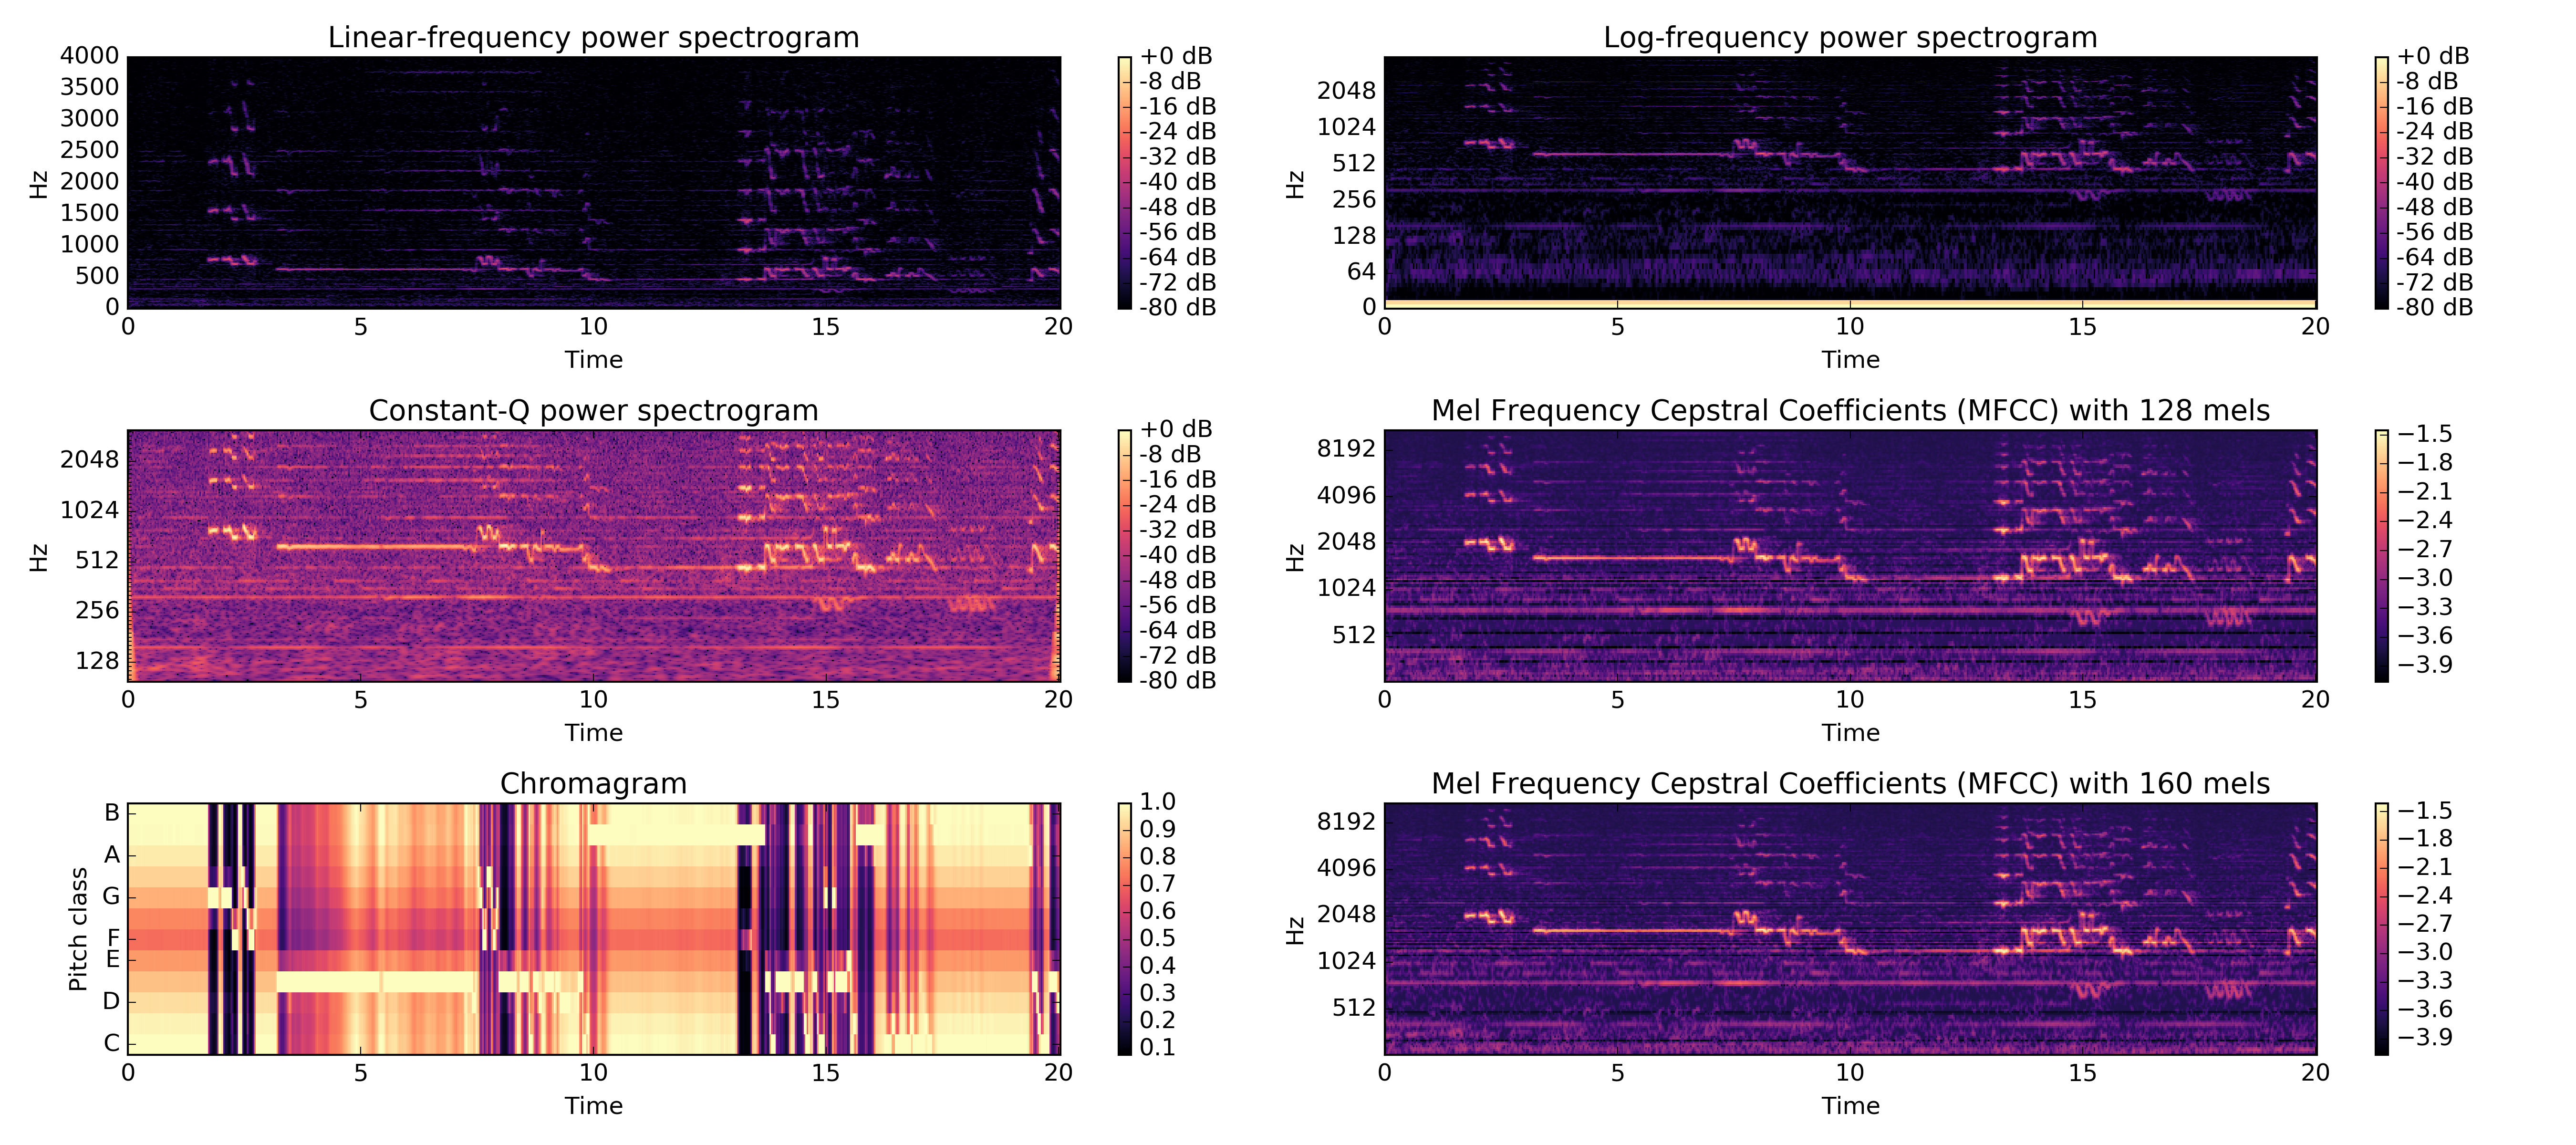
\includegraphics[scale=0.55]{audio_representations.png}
    \caption{Different Time-Frequency representations of the same fragment of carnatic music. In it, a t\=anpura plays a drone, while a flute plays a melody, responded by a violin in seconds 16 and 18.}
    \label{fig:representations}
  \end{sidewaysfigure}


  \subsubsection{Short-Term Fourier Transform (STFT)}

  The basic idea behind the STFT is, instead of performing a single Fourier transform for the whole waveform, to perform many transforms for small, overlapped chunks, a technique called {\it windowing} \cite[p.459]{musimathics}. The frequency resolution is given by the size of that window, and the time resolution by the overlapping factor. And since both parameters are independent from each other, it is possible to get arbitrary precission in both of them. The STFT also provides an inverse transform that allows a perfect reconstruction of the waveform (the exact details needed for a proper implementation can be seen in \cite[ch.10]{musimathics}). See the linear-frequency power spectrogram in Figure \ref{fig:representations} for an example of STFT.\\

  The STFT of a real, discrete analysis of size \(N\), with a window size \(W\) and an overlapping factor of \(O\), outputs a complex-valued matrix of heigth \(W\) and length \(\frac{ON}{W}\). The computational complexity of the STFT of a signal is in \(\mathcal{O}(ON log(W))\).

  \subsubsection{Log-STFT, CQT and MFCC}

  As we have seen, the discrete version of the Fourier transform ``carves up the spectrum of a sound into bins of constant bandwidth. But the sensitivity of the ear to frequency is logarithmic, that is, the ear's sensitivity to pitch diminishes with increasing pitch. From the ear's perspective, the DFT overspecifies high frequencies and underspecifies low frequencies''\cite[p.154]{musimathics}.\\

  This speaks against the criterium for a representation of conveying the relevant information in a convenient and accurate way: with a linear frequency scale, intervals that are perceived as identical have different sizes depending on the register; big portions of the representation convey rather irrelevant data and vice versa.\\

  One approach to overcome this problem is simply to map the vertical axis to a logarithmic scale and interpolate. See log-frequency power spectrogram (Log-STFT) in Figure \ref{fig:representations} for an example. But this doesn't actually solve any of the mentioned issues: the representation of the intervals still varies depending on the register; the lower end becomes very sparse and blurry, and the information in the higher end collapses and is hardly perceivable.\\

  A different approach involves analyzing the waveform with a different set of filters. As already seen, the set of filters that serves as basis for the STFT has the advantage of being linear and orthogonal. But this is mostly an advantage when performing real-time processing, and/or when a lossless signal reconstruction is needed. If none of those conditions apply, as in the case of the preprocessing stage of this thesis, other representations like the CQT and the MFCC may be considered:\\

  The Constant-Q transform (CQT) achieves a representation in which the vertical size of a musical interval remains constant across the whole frequency axis. But not only that: as noted in chapter \ref{about-car}, many musical systems are octave-neutral. The CQT captures this properties by arranging the positions of its filter bank to be repeated periodically every octave. In fact, in its original implementation\cite{cqt}, it is ``equivalent to a \(1/24^{th}\) bank of filters'', that, ``in addition to advantages for resolution, has the advantage that note identification, instrument recognition and signal separation can be done elegantly by a straightforward pattern recognition algorithm''\cite{cqt}. See the Constant-Q power spectrogram in Figure \ref{fig:representations} for an example.\\

  The Chromagram is a derived representation of the CQT: taking advantage of the fact that all the CQT filters are repeated every octave, it collapses all the octaves into one, showing the spectral intensity by pitch. The example of Figure \ref{fig:representations} was performed for 12 filters per octave, and shows clearly how the flute in the audio recording plays the notes G, F,  E${\flat}$ and B${\flat}$.\\


  The Mel Frequency Cepstral Coefficients (MFCC), on the other side, provide a more ``perceptually relevant representation''\cite{choi-robustness}, by  mapping `` the frequencies to the mel scale, which models human perception of changes in pitch, which is approximately linear below 1kHz and logarithmic above 1kHz.''\cite{haggblade}. Similarly to the CQT, it acts like a filter bank (with a more involved computation as further described in \cite{haggblade}), but as it can be seen in Figure \ref{fig:melscale}, the mel scale is not exactly logarithmic.\\

  \begin{figure}[h]
    \centering
    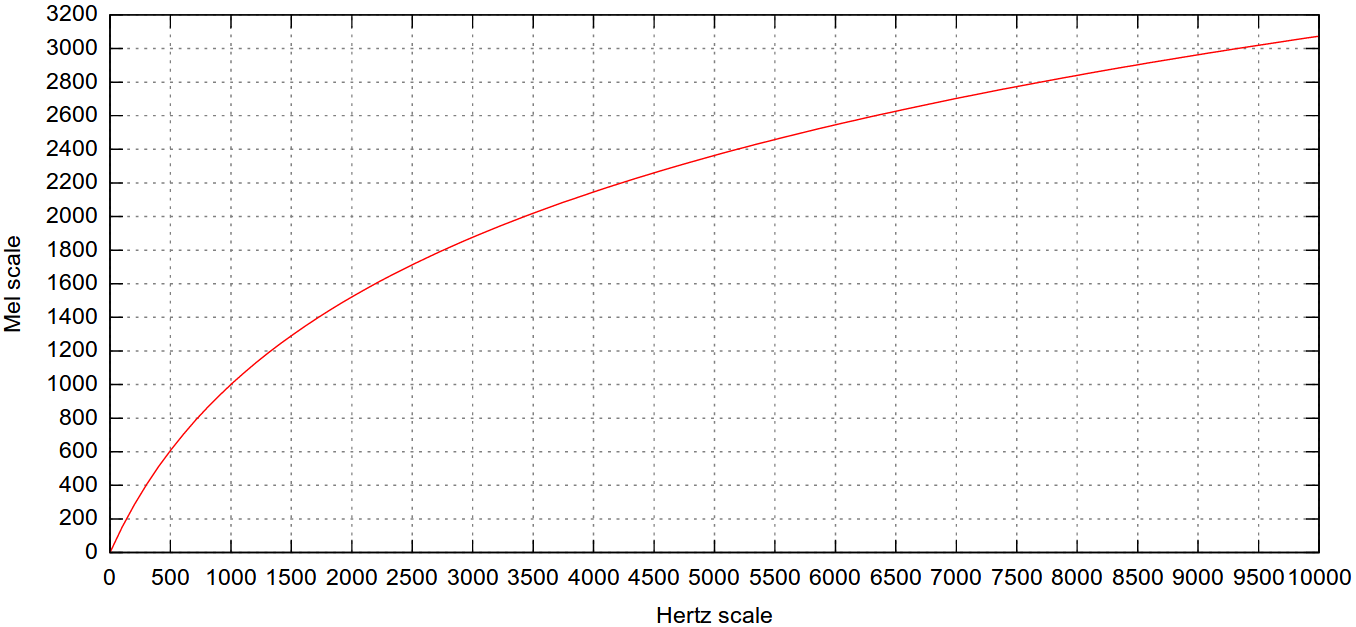
\includegraphics[scale=0.3]{mel_scale.png}
    \caption{A plot of the pitch mel scale versus Hertz scale}
    \label{fig:melscale}
  \end{figure}

  Since both the CQT and the MFCC representations are basically filter banks, their frequency domain is highly customizable, and they can be tweaked to convey the most convenient representation: in the LibROSA implementation, the CQT places the filters across the specified ambitus, with the specified interval resolution in filters per octave. The MFCC, on the other side, requires only the total number of filters to be used, and distributes them evenly across the mel scale. See the fifth section of the \texttt{3\_main\_pipeline.py} Python script for more details.\\

  Another interesting time-frequency representation, and the last one covered here is the one provided by the wavelet transform (WT). It is analogous to the Fourier transform, but instead of complex sinusoidals, the WT is based on wavelets, which are ``discrete families of functions obtained by dilations and translations of a finite number of well chosen moter functions.''\cite[1]{wavelets}. The emphasis is here on the ``well chosen'' attribute: as the sinusoidals, wavelets can also provide a linear orthogonal basis. This allows the nice computational properties as well as a lossless transformation, with the extra advantage of being both frequency and time localized. For that, the wavelet transform is considered ``more appropiate than Fourier series to represent the abrupt changes in non-stationary signals''\cite[1]{wavelets} and is used in many applications in the signal processing field.\\

  The Python script \texttt{6\_wavelet\_test.py} provides an implementation that calculates and plots the STFT and WT of selected .wav files, using the \texttt{PyWavelets} Python module\cite{pywt}. See Figures \ref{fig:rock_stft} and \ref{fig:rock_wt} for a possible output.



  \begin{sidewaysfigure}
    \centering
    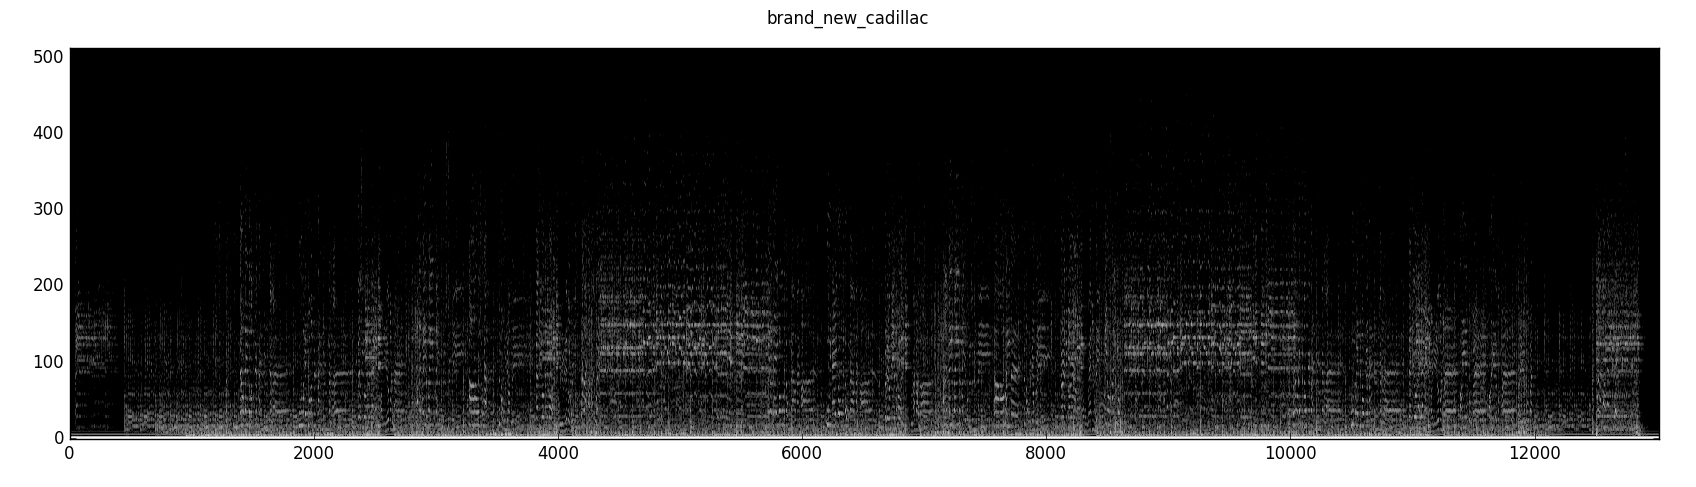
\includegraphics[width=\textheight*9/10,height=5.3cm]{brand_new_cadillac_stft.png}
    \caption{The STFT of a rock song, for a window size of 512, and an overlapping factor of 50\%.}
    \label{fig:rock_stft}
    \vspace{1.6cm}
    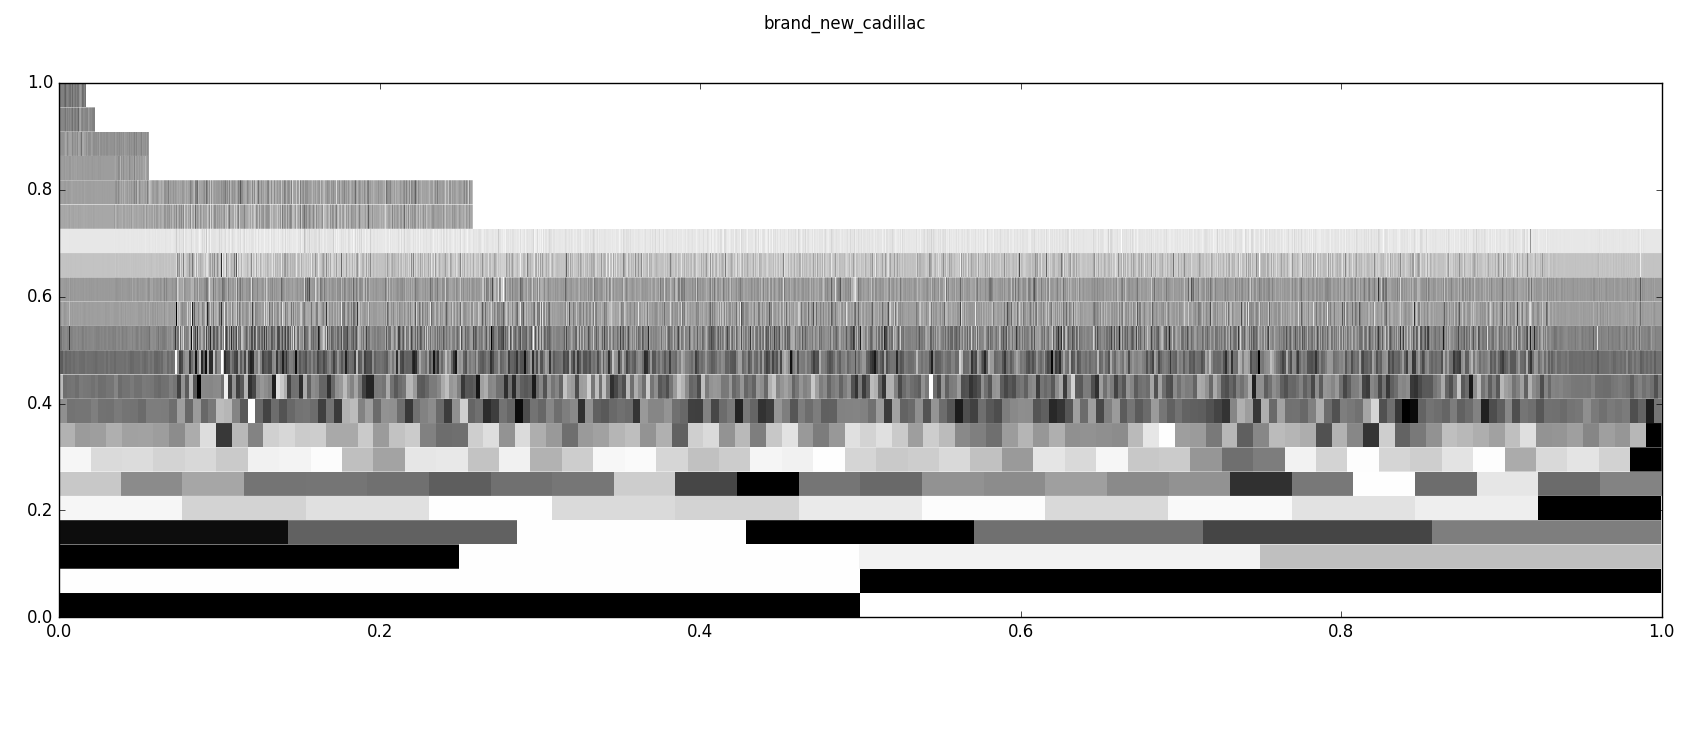
\includegraphics[width=\textheight*9/10,height=7cm]{brand_new_cadillac_wavelet.png}
    \vspace{-0.5cm}
    \caption{The wavelet transform of the same song, computed for the simplest Daubechies wavelet.}
    \label{fig:rock_wt}
  \end{sidewaysfigure}


  \section{Data Splitting} \label{datasplit}

  As explained in \label{crossvalidation}, the machine learning setups usually split the dataset into disjoint subsets. For that, it is important that the distribution of each resulting subset is as similar as possible to the distribution of the whole dataset. The problem that this poses is that, in many cases, a split that is similar with respect to some parameter becomes very different with respect to another.\\

  Take, for example, a set of 10 recordings that has to be fairly split into two equal subsets, having one recording with a duration of 9 hours, and the other 9 recordings being 1 hour long each. Taking apart the 9 hour recording for training and the rest for testing would be a perfect 50\%/50\% split with respect to the total duration, but an awful 90\%/10\% split with respect to the number of samples.\\

  To the best of my knowledge there is no general algorithm that performs a fair split for a given dataset in a fair an efficient way. This is usually a task that is undertaken by highly specialized curators, as in the case of the \(RRD_{CMD}\) dataset described in \ref{rrd_cmd}. For this thesis, I implemented two algorithms, described in the following sections.

  \subsubsection{First Approach}
  The splitting algorithm contained in the \texttt{4\_data\_split\_alt.py} Python script implements a heuristic that intends to promote a healthy balance between quantity and variety of the data in both resulting subsets. Given the set to split and the desired proportion, loops over the samples (sorted from smallest to biggest), performing the split by the given ratio until the proportion is achieved or surpassed. Such an approach could be useful only if the dataset has classes with very few samples and high duration variance.

  \subsubsection{Second Approach}

  This approach is followed by the \texttt{split\_labels} function in section seven of the \texttt{3\_main\_pipeline.py} Python script. This approach is based only in the number of recordings, and disregards the total duration of the resulting splitted subsets. It also includes further mechanisms to reject unfeasible splitting ratios or prevent splits resulting in any class having no representation.



  \section{Data Augmentation}\label{data-augm}

  Data augmentation is a form of regularization consisting in creating fake data and add it to the training set\cite[p.240]{goodfellow}.Further quoting, ``This approach is easiest for classification. A classifier needs to take a complicated, high dimensional input \(x\) and summarize it with a single category identity \(y\). This means that the main task facing a classifier is to be invariant to a wide variety of transformations. We can generate new \((x,y)\) pairs easily just by transforming the \(x\) inputs in our training set''.\\

  One of the problems that data augmentation can help to solve is class imbalance of the training set: when one class has more data than other (inter-class imbalance), or specific samples of one class are much bigger than others (intra-class imbalance),  random sampling from the training set will cause the model to overfit the most represented regions of the sample space. In order to solve this, there are four popular strategies:\\

  The most straightforward is to truncate the overrepresented classes. This is undesirable since data is the currency of machine learning, and should not be thrown away if it can be avoided.\\

  A more popular option is to balance the cost function by introducing a weight that is inversely proportional to the representativity of the given training sample. Since gradient descent bases its steps on the derivative of the cost function, this strategy naturally balances the learning process.\\

  Another option is to force data redundancy, by, for example, picking the same amount of information from every class each time. This will cause the data in the underrepresented classes to appear more often.\\

  Data augmentation works similarly to the data redundancy, but instead of reappearing identically, some transformation is applied to it. This transformation has to be chosen very carefully, as it has to be feasible for the problem domain in question. For instance, in an OCR application, linear transformations like stretching and scaling are feasible, but symmetrical rotations along the vertical axis are not.  This is well summarized in the following sentence: ``it is difficult to generate new fake data for a density estimation task unless we have already solved the density estimation problem''\cite[p.240]{goodfellow}: augmenting the data implies a somewhat explicit knowledge of the ground truth, but is {\it not} the ground truth (otherwise it wouldn't be necessary to perform any kind of machine learning since the problem would be solved). This is also why augmentation should never be applied to the validation or test datasets: testing on augmented data would assert whether the model has learned the augmentation paradigm and would skew the diagnose.

  \subsection{Augmentation Paradigms}

  For the r\=aga classification, I considered basically three strategies: noise injection, time stretching and frequency transposition.\\

  The first one is effective for speech recognition tasks\cite[p.241]{goodfellow}, and could be feasible here too, but I refrained from implementing it since most of the recordings that I checked are already very noisy.\\

  Frequency transposition is a feasible data augmentation paradigm for carnatic music, due to the fact that the fundamental frequency is an arbitrary factor, as already exposed in chapter \ref{about-car}.\\

  At first sight, time stretching seems feasible too: mildly changing the speed of a certain fragment shouldn't have a deep impact in its identity. But, as the temporal aspects do play a role in the definition of the r\=agas, this has to be done very carefully. Figure \ref{fig:chalan-stretch} illustrates that conveniently.

  \begin{figure}[h]
    \centering
    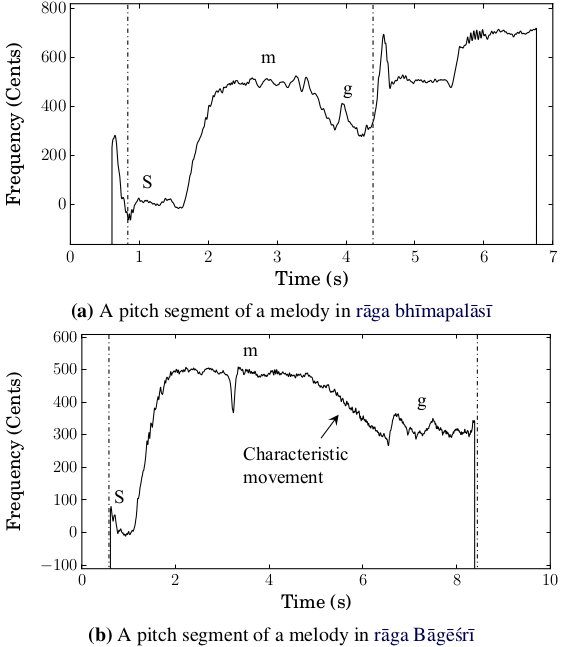
\includegraphics[scale=0.6]{chalan_stretch.png}
    \caption{Impact of temporal aspects in the r\=agas. Although the melodic transition in both r\=agas is made through the same set of svaras S, m, and g, in the same order, the characteristics of the transition regions in the melody and the duration of the svaras are different (from \cite[p.22]{gulati}).}
    \label{fig:chalan-stretch}
  \end{figure}


  \subsection{Implemented Augmentation}

  The \texttt{5\_data\_augmentation\_alt.py} Python script implements an augmentation algorithm that, by applying arbitrary transposition and stretching to given wav files, promotes intra-class and inter-class balance. The heuristic for the balance is very similar to the first approach explained in \ref{datasplit}.\\

  Note that the transposition and stretching factors are independent from each other. To achieve that, the script calls the third-party program \texttt{Rubber Band}\cite{rubberband}.


  \section{Data Feeding}\label{data_feeding}

  Once the required data has been loaded to the RAM, it has to be fed to the model. When performing stochastic gradient descent (explained in \ref{graddesc}), the model accepts data in the form of a batch, which is basically a vector of tensors. For that, the \texttt{3\_main\_pipeline.py} Python script implements two functions: \textt{get\_random\_batch} and \textt{cut\_sample\_to\_chunks}.\\

  The first one implements the functionality already explained as the ``data redundancy'' approach, in section \ref{data-augm}. This function is expected to be suitable for the training phase, since it provides a fair inter-class and intra-class balance:  for each element of the batch, all the classes have the same random probability of being represented, and the same happens for all the samples within a class. The sample is also expected to be fairly represented in the long run, since the position of the window extracted from it is also drawn from a random uniform distribution.\\

  The second one cuts a given sample of arbitrary size into chunks of the specified size, discarding the last chunk if it is smaller than the rest. This paradigm is more suitable for validation and testing purposes, since it allows an efficient and flexible implementation of voting mechanisms (voting only makes sense among chunks of the same sample, more details in section \ref{errormetrics}), and it doesn't matter that all the chunks belong to the same class, since the whole subset will be processed and taken into account for the error metrics.



  \section{Model Implementation}

  In every supervised learning setup, there is a set of tasks that has to be repeated almost identically every time, regardless of the exact model or parameters being used. Specialized machine learning libraries like TensorFlow, described later, help to take care of many of these tasks.\\

  On a higher level, the tasks concerning the implementation of the model can be encapsulated into three functional groups: definition, training and testing. The software patterns resulting from that encapsulation are also described in this section.\\

  Visualizing the results can be also very helpful for debugging the model and interpreting its results. TensorBoard, explained at the end of the section, provides good functionality for that.

  \subsection{About TensorFlow}

  TensorFlow is an open source software library for numeric computation developed by Google\cite{tflow}. Originally developed for conducting machine learning and deep neural networks research, it makes very easy to work with GPUs, and has a broad built-in support for machine-learning related functionality. Tensorflow organizes the computation using data flow graphs: ``nodes in the graph represent mathematical operations, while the graph edges represent the multidimensional data arrays (tensors) communicated between them''\cite{tflow}.

  \subsubsection{Lifecycle and Namespaces}

  Most of the functionality of TensorFlow is written in C++. Therefore, the Python programs using TensorFlow have two distinct parts: building the computational graph (which has to be compiled into C++ and is statically typechecked) and running it.\\

  In order to access the previously compiled nodes, TensorFlow provides a global namespace system, which can be visited with the \texttt{get\_tensor\_by\_name} function or by applying Python's \texttt{with} context manager to the corresponding object (usually a \texttt{Graph} instance, a \texttt{Session} instance or a call to the \texttt{tf.name\_scope} function).



  \subsubsection{Building the Graph}

  The dataflow in a \texttt{Graph} usually starts with a \texttt{constant}, a \texttt{Variable} or a \texttt{placeholder} nodes, which are designed to contain tensors. The contents of the constant are statically bound when compiling the graph and cannot change. The contents of the Variable are more flexible: they can be updated while running the graph but have to be initialized for a fixed shape at the beginning of the session. The placeholders are the most flexible of all, since they don't have to be initialized: At the moment of evaluating the contents of a node, the mapping from every placeholder involved in the computation to its corresponding data has to be provided in the form of a dictionary called the \texttt{feed\_dict}. This matches very well the functionality described in section \ref{data_feeding}.\\

  The connection from one node to another is expressed by passing the existing node as an argument to the constructor of the following node. Mirroring the functionality of NumPy, TensorFlow provides support for most arithmetic and memory operations, as well as many machine-learning related computations, so most of the mainstream models (like neural networks) are very straightforward to implement. As an example of how to build a graph, see the function \texttt{make\_custom\_graph} in the \texttt{3\_main\_pipeline.py} Python script.\\

  Among the most specialized built-in nodes are the optimizers: when an optimizer is positioned in the graph (usually by passing a cost function to it), TensorFlow traverses all its underlying nodes, attaching the corresponding optimization operation to it (for the gradient descent optimizers, this is the backpropagation algorithm), and keeping track of the variables that it finds. Then, when its \texttt{minimize} method is run, the optimization is computed through the attached nodes, and the tracked variables are updated with the optimized values. See \cite[p.212]{goodfellow} for a more detailled explanation.


  \subsubsection{Running the Graph}

  The process of running the previously compiled graph is managed by an instance of the \texttt{Session} class, via its \texttt{run} method, which accepts a node or list of nodes as its first argument. Calling run for a node will traverse down the graph until reaching the initial nodes. Then, followning the topological ordering of the graph, the computation is propagated forward, until all the values for the required nodes are eventually calculated and returned by the method.\\

  The function \texttt{run\_training}  in the \texttt{3\_main\_pipeline.py} Python script illustrates how this can be done. Note that if any of the initial nodes is a placeholders, a value for it has to be provided in the feed\_dict.


  \subsection{Model Definition}

  All the models defined in the \texttt{3\_main\_pipeline.py} Python script are expected to receive a batch of data with its corresponding batch of labels, and some extra hyperparameters like, for example, the dropout rate to be applied. Then, they use their parameters, stored in variables, to propagate the given data and produce a hypothesis in the form of a logit vector, which is returned together with the L2 loss for all the model's parameters excluding the bias.\\

  If the model is defined in accordance to this interface, the \texttt{make\_custom\_graph} function will be able to integrate it successfully. This function takes care of creating a graph with the following functionality, common to every model:

  \begin{itemize}
  \item creates the placeholders for the different input batches and hyperparameters
  \item integrates the specified model and defines the cost function for it, with the given L2 regularization hyperparameter.
  \item instantiates the specified optimizer with the given learning rate, and sets it to optimize the cost function above mentioned.
  \item implements some basic metrics like correct predictions and mean accuracy of the given batch.
  \end{itemize}

  The function returns then the whole graph, as well as two dictionaries; one with the input nodes and one with the outputs.

  \subsection{Model Training}

  Following the idea of the  \texttt{make\_custom\_graph} function,  \texttt{run\_training} intends to provide a simple yet highly customizable interface to the user. Its parameter list is the following:

  \lstset{language=Python}
  \lstset{basicstyle=\footnotesize}
  \begin{lstlisting}

    def run_training(train_ddict, cv_ddict, test_ddict,
    model, optimizer_manager,
    batch_size, chunk_size, l2rate_fn, dropout_fn,
    log_path,
    batch_freq=100, cv_freq=500,
    cv_voting_size=1, test_voting_size=1,
    max_steps=float("inf"),
    extra_info="",
    normalize_chunks=True,
    max_gpu_memory_fraction=1)
  \end{lstlisting}

  Most of its parameters are self-explanatory: this function instantiates the graph for the given model, optimizer and hyperparameters. Then starts the session, and then runs the training loop. Every iteration loads a batch provided by \textt{get\_random\_batch} and trains the model by running the optimizer. Also, the statistics for the training and validation steps are output with the specified frequency.\\

  The \texttt{OptimizerManager} class is simply a wrapper for the existing tensorflow optimizers, to allow a better integration in the graph. Note that the regularization, dropout and learning rate hyperparameters are to be passed as functions that accept the current training step as parameter. This allows to model arbitrarily complex behaviors (like, for example, learning rate decay) without any structural changes in the code.

  \subsection{Model Testing}

  Every \texttt{cv\_freq} steps, the whole validation set is evaluated. This is done by converting all of its records to batches with \texttt{cut\_sample\_to\_chunks}, feeding the batches to the graph (by the specified \texttt{cv\_voting\_size}) and storing the results into an instance of the \texttt{ConfusionMatrix} class, which keeps track of the results and provides functionality for calculating the total and the by-class accuracy.\\

  When the whole subset has been tested, it is possible to create and export a plot of the matrix with the \texttt{add\_confmatrix} method of the \texttt{TensorBoardLogger} class.

  \subsection{Visualization with TensorBoard}  \label{tb-visualization}

  TensorBoard is a suite of visualization tools designed to run on a HTTP server, that can be then visited by a web browser. It provides real-time information on the implemented model, by showing its computational graph as well as the functions, images, audio files and/or histograms that it may generate. For that, the server visits a log directory that has to be specified when it starts with the \texttt{--logdir} flag, and serves to a given IP address (\texttt{localhost:6006} by default).\\

  This log directory contains a set of protocol buffers\cite{protobufs}, which are basically extensible strings that contain data like functions, images, audio files, as well as the metadata attached to them like date and title. This buffers are generated and interactively expanded by the \texttt{tf.summary.FileWriter}, and the contents are represented in TensorFlow by the \texttt{tf.Summary} objects.\\

  The \texttt{TensorBoardLogger} class in the \texttt{3\_main\_pipeline.py} Python script provides an implementation that outputs functions and matrix plots to the specified log directory.\\

  In some cases, the computer holding the log files is only accessible via SSH and prevents visiting the TensorBoard HTTP server. In that case, SSH tunneling can be performed: The following command forwards TensorBoard to \texttt{localhost:16006}, assuming it was started with the default IP address:\\
  \texttt{ssh -p <PORT> <USER>@<SERVER> -N -f -L localhost:16006:localhost:6006}


\chapter{Experiments and Results}\label{experiments}
After describing in chapter \ref{implementation}, the tools and ideas that I used and developed for the implementation of this thesis' setup, this chapter reports the specific experiments that I conducted using those tools, in order to explore the problem definition as discussed in chapter \ref{problem-def}.\\

For that, the chapter will follow an iterative structure: For each conducted experiment, the specific settings and motivations behind them will be described, followed by the obtained results, and finally, the conclusions that led to the subsequent experiment will be exposed. The decisions that I made are based in the domain-specific and technical knowledge presented in chapters \ref{about-ds},\ref{about-car}, \ref{context} and \ref{about-ml}.

Note that the following general considerations apply to the whole chapter:
\begin{itemize}
\item All the Python scripts can be found under the https://github.com/andres-fr/bachelor-thesis/code/ link.
\item The data and the labels can be found under the https://github.com/andres-fr/bachelor-thesis/datasets/ link.
\item The result logs are located in the corresponding \texttt{<PROJECT>/logs*} directories, wich can be consumed by TensorBoard as explained in section \ref{tb-visualization}.
\item The experiments and preprocessing were conducted on a server with an {\it Intel(R) Core(TM) i7-5930K CPU @ 3.50GHz} CPU, an {\it Nvidia GeForce GTX 1080} GPU and 128GB RAM.
\end{itemize}


\subsubsection{I. MNIST}

I started with this very well-known classification problem to made sure that the flexibility of my setup didn't hinder its effectivity. MNIST is a simple labeled dataset that contains images of hand-written digits in the form of 28x28 matrices, and divided in 55000 training samples, 5000 validation samples and 10000 test samples comprising 10 classes (the digits from 0 to 9).\\

In order to test it on my setup, I just had to add two things: the \texttt{load\_mnist\_as\_ddicts} data loader function, which adapted the native MNIST format to my data format (as explained in chapter \ref{implementation}), and the neural network architecture described in TensorFlow's ``Deep MNIST for Experts'' tutorial\cite{tf-cnn}, which I re-implemented in the \texttt{mnist\_model\_conv}. The architecture of the model is described in Table \ref{fig:mnist-arch}.\\

\begin{table}
  \centering
  \resizebox{\textwidth*1/2}{!}{%
    \begin{tabular}{*2l}\toprule
      \bfseries Layer  & \bfseries Shape\\\Midrule
      Input &       28\times28\times1\\\Midrule
      Conv5x5 &       28\times28\times32\\%\Midrule
      MaxPool2x2 &    14\times14\times32\\\Midrule
      Conv5x5 &       14\times14\times64\\%\Midrule
      MaxPool2x2 &    7\times7\times64\\\Midrule
      FullyHidden &   7\cdot7\cdot64\times hidden\_size\\\Midrule
      Logits &        hidden\_size\times num\_classes\\\Midrule
  \end{tabular}}
  \caption{The deep NN architecture suggested in \cite{tf-cnn}. There are ReLU layers between convolution and pooling. There is a ReLU and a dropout layer before the logits, in that order.}
  \label{fig:mnist-arch}
\end{table}

The results were the ones expected for a working setup: training an adam optimizer with an initial learning rate of \(10^{-4}\), a batch size of 200, no dropout and a L2 regularization factor of \(3\cdot 10^{-7}\) led to an accuracy consistently over 97\% on the test, with no voting and after training for less than one epoch (which took less than 1 minute on the hardware specified above). Switching to the simpler SGD and momentum optimizers led to similar results but a much slower convergence rate.\\

Since the pipeline consists of many elements connected in series, a pipeline working as expected is a strong indicator (but not a proof) that all of its elements are working as expected. This includes the data feeding model, the graph generation, the model implementation and integration, the optimization mechanism and the error metrics system.\\

\subsubsection{II. Rock vs. Merengue}

In this second stage of the experimental phase, I tested some of the implemented storage, conversion and representation segments of the pipeline, by working with music instead of handwritten digits. But before taking samples from the carnatic dataset, I opted for testing on a much simpler problem space, by collecting a few rock&roll and merengue songs, and classifying between them.\\

This problem was expected to be much easier than r\=aga classification, since this two genres are not only clearly distinguishable, but they also very consistent in their characteristical features (f.e. instrumentation, harmony, rhtythmic patterns and structure). The selected dataset features 80 songs, 40 of each class. The selected songs are very characteristical of their genre and feature different bands, singers and tonalities.\\

After reading some of the related work described in chapter \ref{context}, I considered meaningful to train end-to-end models based on the raw waveform, as well as models based on the STFT of the waveform. The two applied architectures, defined in the  \texttt{model\_conv1d} and \texttt{model\_conv2d} functions of the \texttt{7\_rock\_vs\_merengue.py} script, responded to the only requirement of having to fit such data (conv1d for the one-dimensional waveforms and conv2d for the STFT), and to be able to learn meaningful features of both classes.\\

For instance, the model trained on the raw waveforms obtained an accuracy consistently above 80\%, using an adam optimizer with an initial learning rate of \(10^{-4}\), a dropout of 50\%, a L2 regularization rate of 0.3 and batches of 100 randomly selected 2-second chunks. Since this classification problem wasn't the main focus of this thesis, I didn't put an emphasis on optimizing the results, or finetuning the architectures.\\

At that point, it sufficed for me to note that both models performed noticeably better than pure random guessing; so, after looking at some plots like the ones showed in Figure \ref{fig:representations} and \label{fig:rock_wt}, I assumed that the conversion, storing and loading operations as well as the different representations for the musical contents worked as expected, and I decided to move onto the carnatic corpus.


\subsubsection{III. Augmented Carnatic Corpus}

For the first batch of experiments, I preprocessed the training data by timestretching it as explained in section \ref{data-augm}. This yielded a HDF5 file that, with the highest zip compression index, occuped over 300GB of disk memory. The (parallelized) computation of this augmentation with the processor specified above took over 12 hours, and loading the data to the RAM took about 4-5MB per second.\\

The rationale behind this data augmentation, as explained, was to enhance intra- and inter- class balance while not enforcing data duplication: mild time stretches were assumed to enhance generalization ability. Also, I fixed the chunk duration to 20 seconds, which seemed also a feasible size to contain r\=aga relevant information.\\

In order to select the representations and architectures I regarded two factors, which are codependent: the reported efficiency of the representation and the reported efficacy of the network, based on its performance, size and required training time. Among all the combinations, the fully-convolutional architectures reported in \cite{choi-fcn} and explained in chapter \ref{context} based on the MFCC representation with 128 filters seemed a good start.\\

For instance, the \texttt{fcn4} function of the \texttt{3\_main\_pipeline.py} Python script is a close implementation of the paper's FCN4 network, slightly adapted to fit the exact dimensions (128 height and 860 width).\\

It followed a series of experiments in which no combination of hyperparameters was able to learn meaningful features at all. I tried all the different variations of the FCN architecture present in the \texttt{3\_main\_pipeline.py} script, with SGD, Momentum and Adam optimizers (choosing learning rates below \(10^{-4}\) and training for at least 150000 optimization steps), and applied grid search for the regularization L2 and dropout rates.\\

The observed behaviour was always the following: The different regularization strategies, as well as the network capacity, had an impact in the network's ability and celerity in fitting the training data. Lower L2 and dropout rates with bigger models lead to good training but bad validation results (overfitting), and increasing this regularization measures would only decrease the training results, without increasing the validation accuracy.\\

Such bad results are not only discouraging but also difficult to interpret, so I decided to minimize the problem space, in order to have some more control on the data space and discard the possibility of a flaw in the augmentation process.

\subsubsection{IV. RRD\(\boldsymbol{^*}\) Dataset}

In order to decrease the problem space, I drastically reduced the data space: instead of taking the whole corpus, I focused on the \(RRD^*\) dataset, which, as explained in section \ref{rrd_cmd}, has been curated by Gulati et al. following, among others the criteria of completeness and quality. Since this is a dataset that he uses for testing purposes, it is much more balanced across classes, and the hope was that it would contain a selection of the most characteristic samples of the problem space, facilitating the learning of the relevant features. Eventually, I also reduced the amount of classes to two, by taking special care in choosing r\=agas that are well represented and share a minimal set of svaras (see Figure \label{fig:rrd-ragasvaras} and the \texttt{raaga\_list.txt} file for more details).\\

It followed a batch of experiments analogous to the ones that I did in III, with similar results: Figures \ref{fig:tb-overfit} and \ref{fig:confmatrices} exemplify for this minimal 2 class setup the inability of the tested models to capture the features relevant for r\=aga classification, regardless of the amount of regularization.\\

This behaviour can be described as overfitting: note that the model learns features that are orthogonal to the r\=aga invariances, which can be observed in the fact that, although the accuracy on the training data may rise, the distribution for all columns in the confusion matrix is proportional, and far away from the ``independence'' among rows and columns that a confusion matrix displays for a successful classification.


\begin{figure}[h]
  \centering
  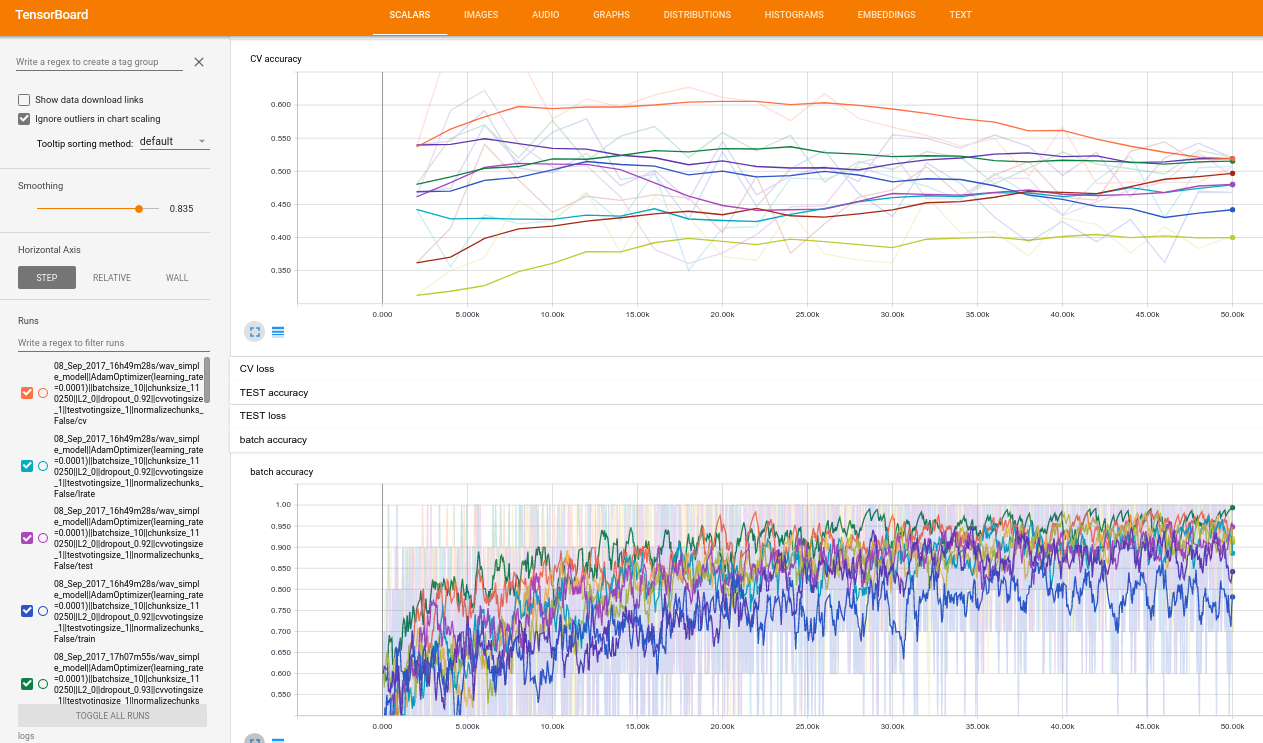
\includegraphics[scale=0.33]{tb_overfit.png}
  \caption{The validation (above) and batch (below) accuracy for many different models tested on two classes of the \(RRD^*\) dataset.}
  \label{fig:tb-overfit}
\end{figure}




\begin{figure}
  \centering
  \begin{subfigure}[b]{0.48\textwidth}
    \centering
    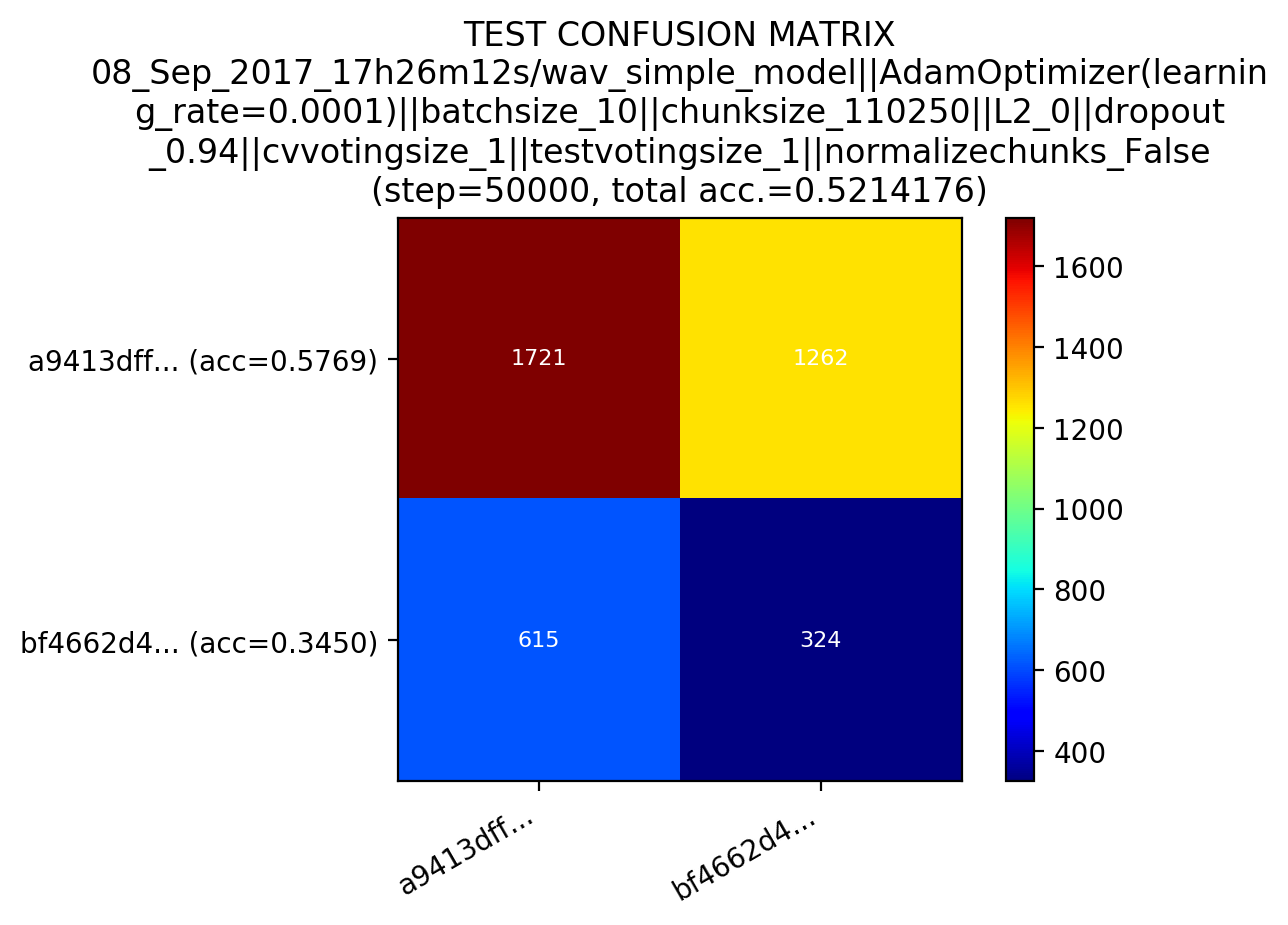
\includegraphics[width=\textwidth]{confmat1.png}
  \end{subfigure}
  \hfill
  \begin{subfigure}[b]{0.48\textwidth}
    \centering
    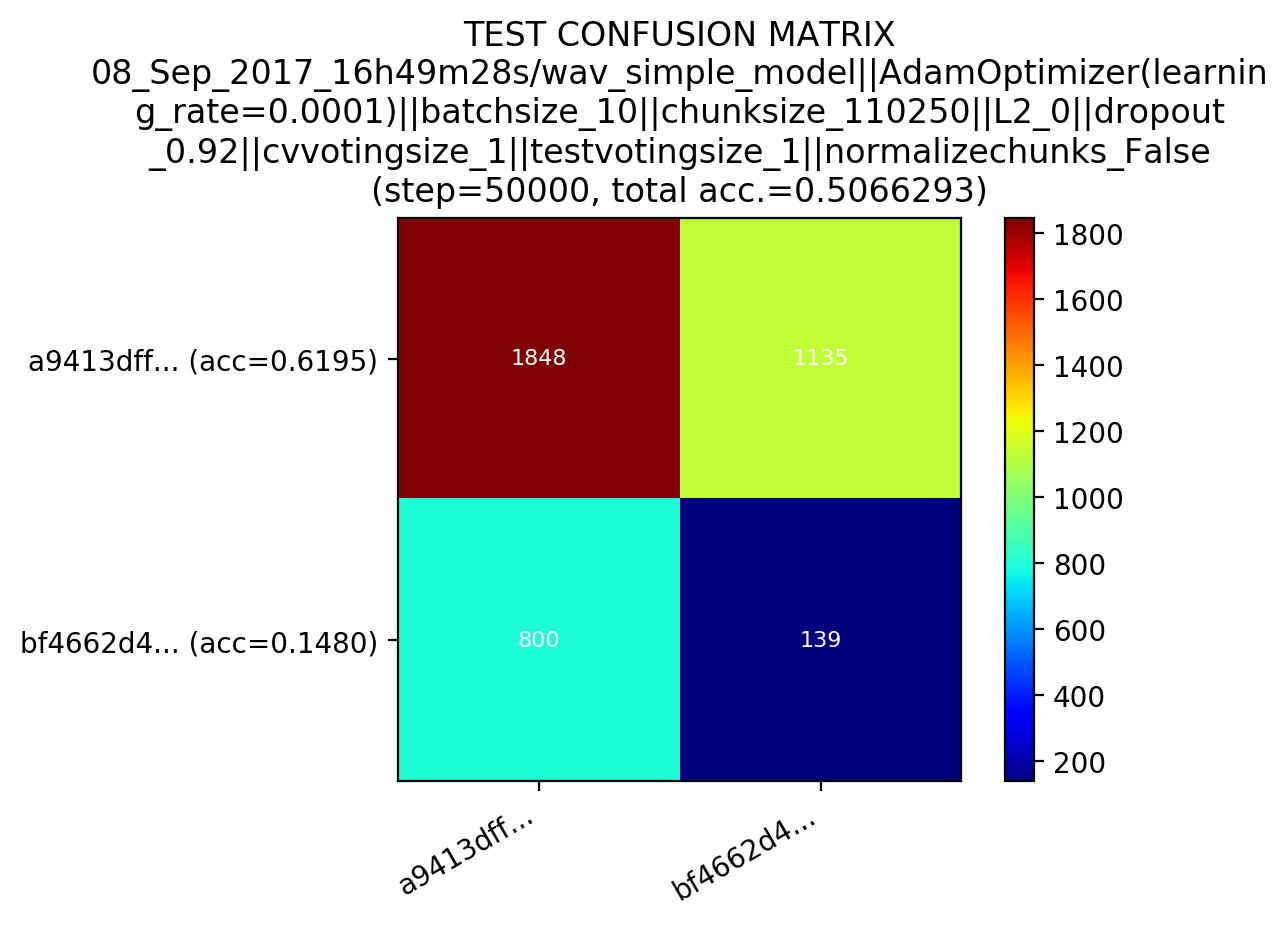
\includegraphics[width=\textwidth]{confmat2.png}
  \end{subfigure}
  \hfill
  \caption{The confusion matrices for two different models tested on two classes of the \(RRD^*\) dataset.}
  \label{fig:confmatrices}
\end{figure}


\chapter{Conclusions and Future Work}\label{conclusion}
In the present thesis I performed end-to-end, supervised learning with neural networks to learn and perform r\=aga classification based on the Dunya corpus of carnatic music and on the \(RRD^*\), a smaller subset of it.\\

In this context, and contravening the precepts of the CompMusic project, I explicitly refrained from applying domain-specific solutions: the models and concepts that I applied were mainly based on literature that follows more closely the mainstream of the machine learning field. Whereas I based some of the decisions (like the duration of the datachunks or the augmentation model) in domain-specific musical aspects, these remain very general and could apply as well for many other domains.\\

The preprocessing stage remained as well very general, in order to leverage and test the capacity of such neural networks to learn meaningful information in the context of r\=aga classification. The results of the experiments were that the different tested setups were unable to learn any relevant features for this task.\\

Without excluding practical explanations for this (like flaws in my thinking process and/or implementation), one possible explanation could be that the sparseness of the relevant r\=aga information across the chosen representations used makes the learning process extremely inefficient and error-prone. The importance of a dense representation can be clearly seen in the state-of-the-art approaches (see section \ref{context_raaga}), and especially in the  the TDMS representation, which ``improves the accuracy of r\=aga recognition by large margins, without the use of any elaborated classification schema''\cite[p.192]{gulati}.\\

In order to allow a neural network to learn such specialized and sparse features (and assuming this explanation as valid), two possible strategies could be to feed more data (by collecting it or via some feasible augmentation paradigm) and/or applying a more efficient preprocessing approach (for example cutting out the non-melodic sections).\\

Also, for a better diagnose of the problems presented here, analyzing the histograms for the different convolutional weights, and applying the auralization techniques explained in \cite{choi-explaining} would definitely be two strategies worth exploring.


%%%%%%%%%%%%%%%%%%%%%%%%%% APPENDIX
\appendix



\chapter{Dataset Statistics} \label{ds-stats} %***
\begin{sidewaysfigure}[H]
  % \hspace*{-0.6cm}
  \centering
  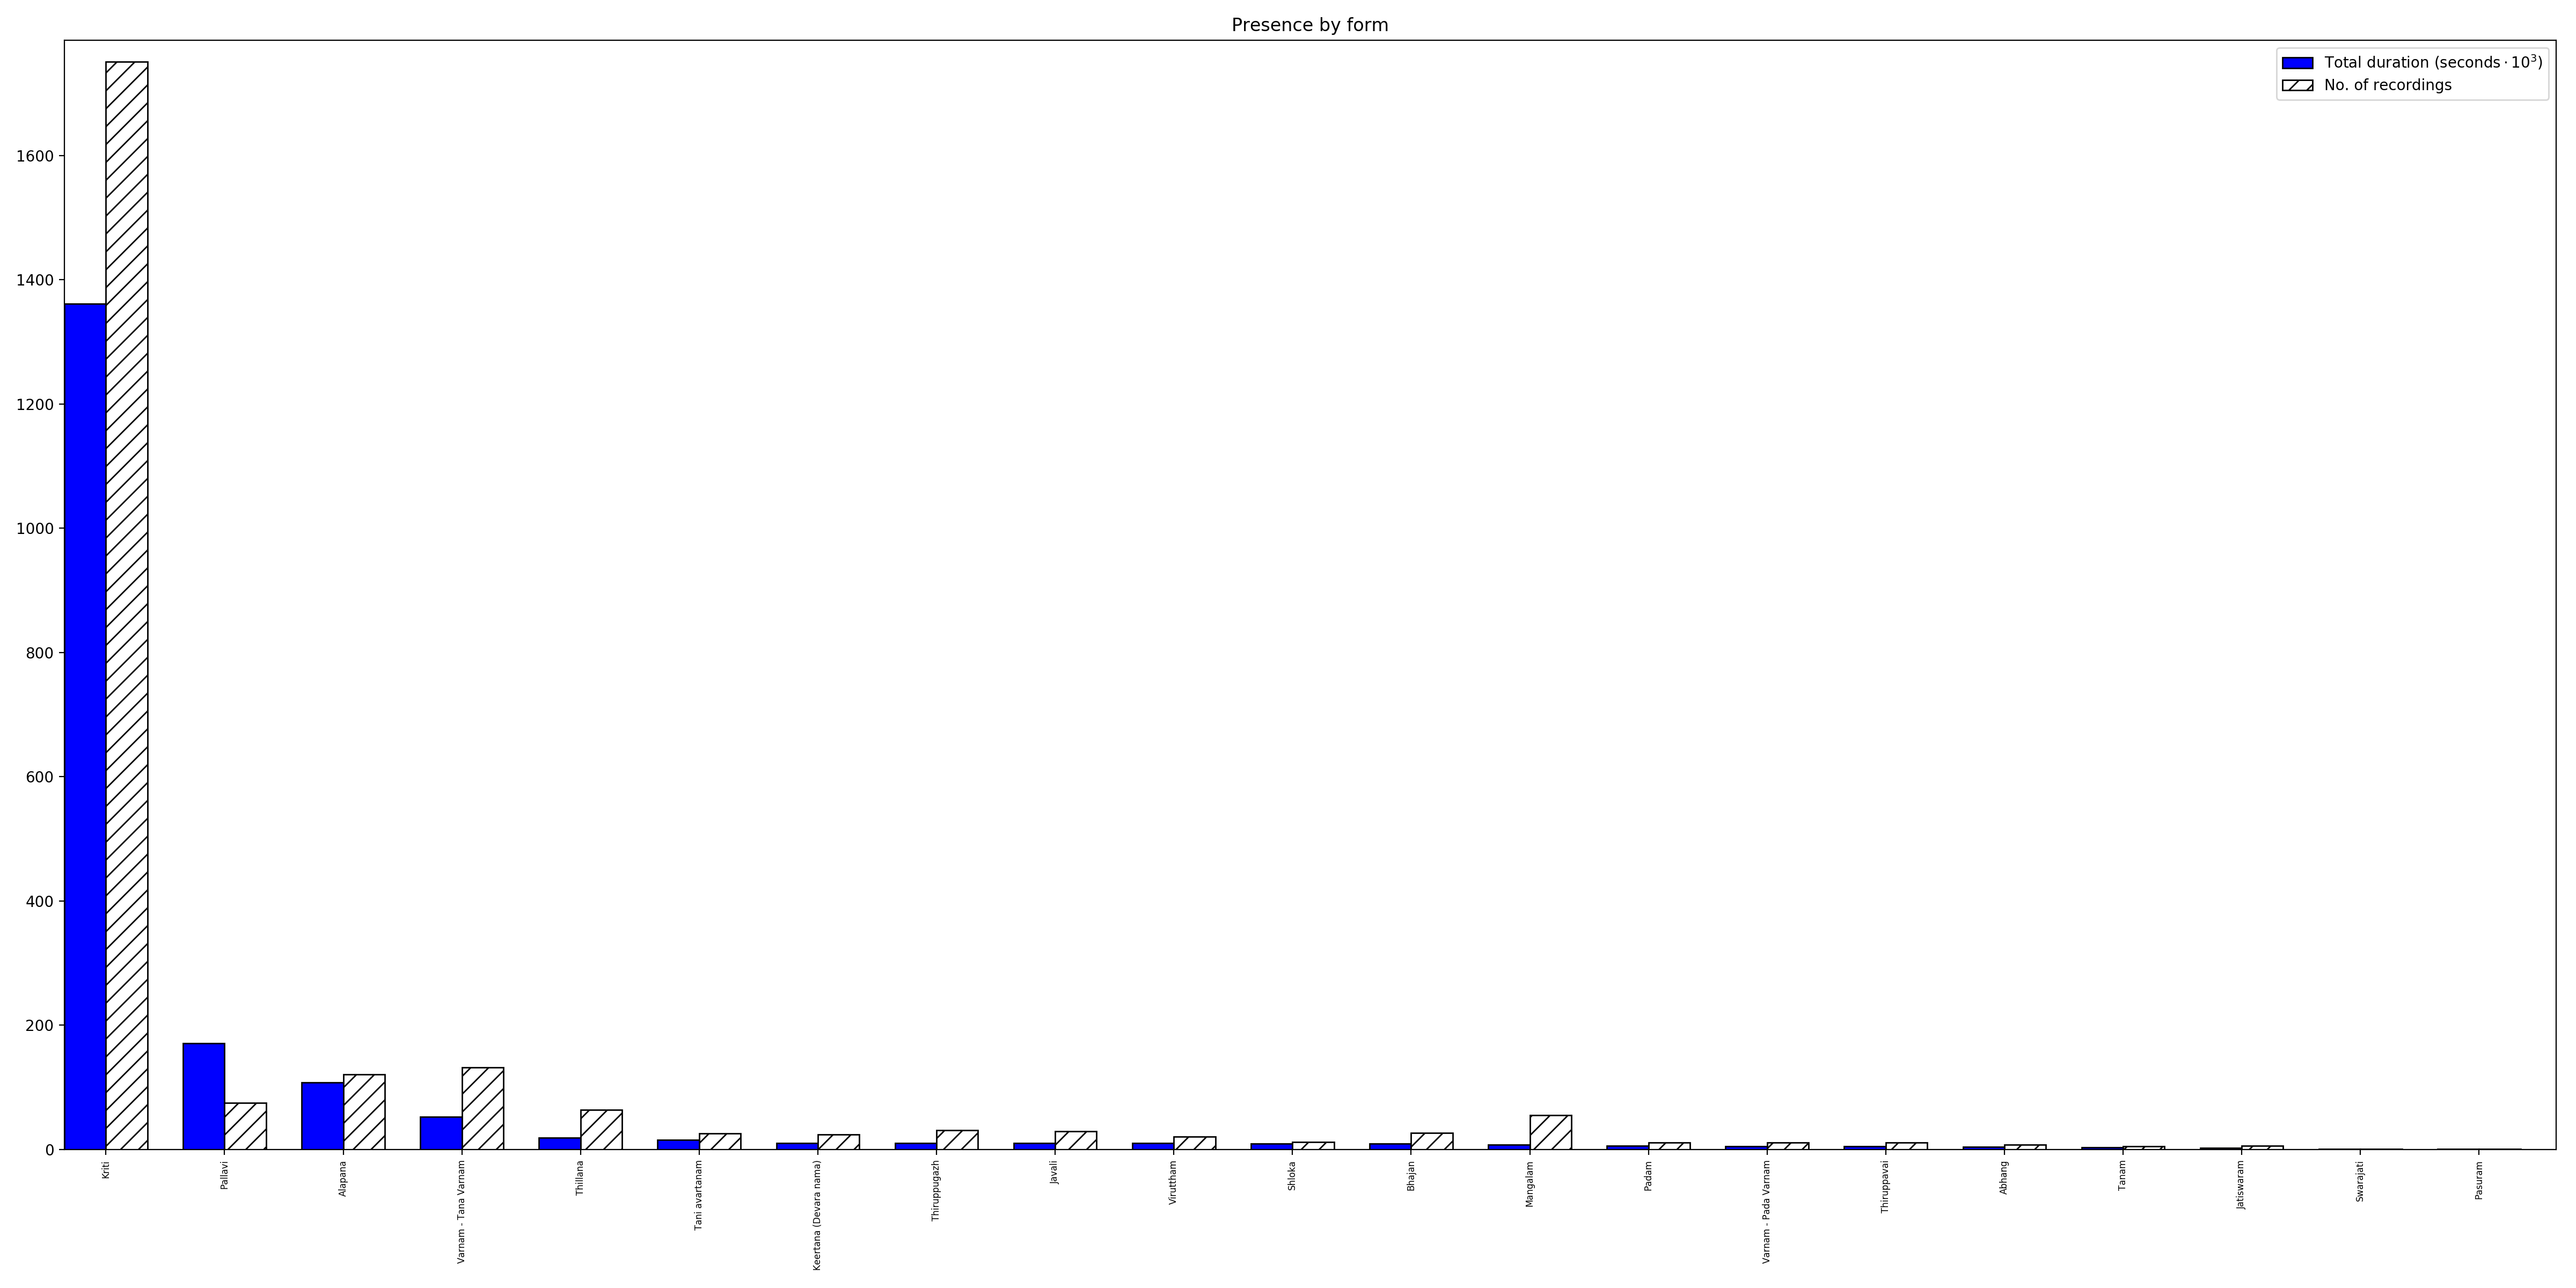
\includegraphics[scale=0.41]{histogram_form.png}
  \caption{The number and total duration of the recordings labeled with form.}
  % \label{fig:_}
\end{sidewaysfigure}

\begin{sidewaysfigure}%[h]
  % \hspace*{-0.6cm}
  \centering
  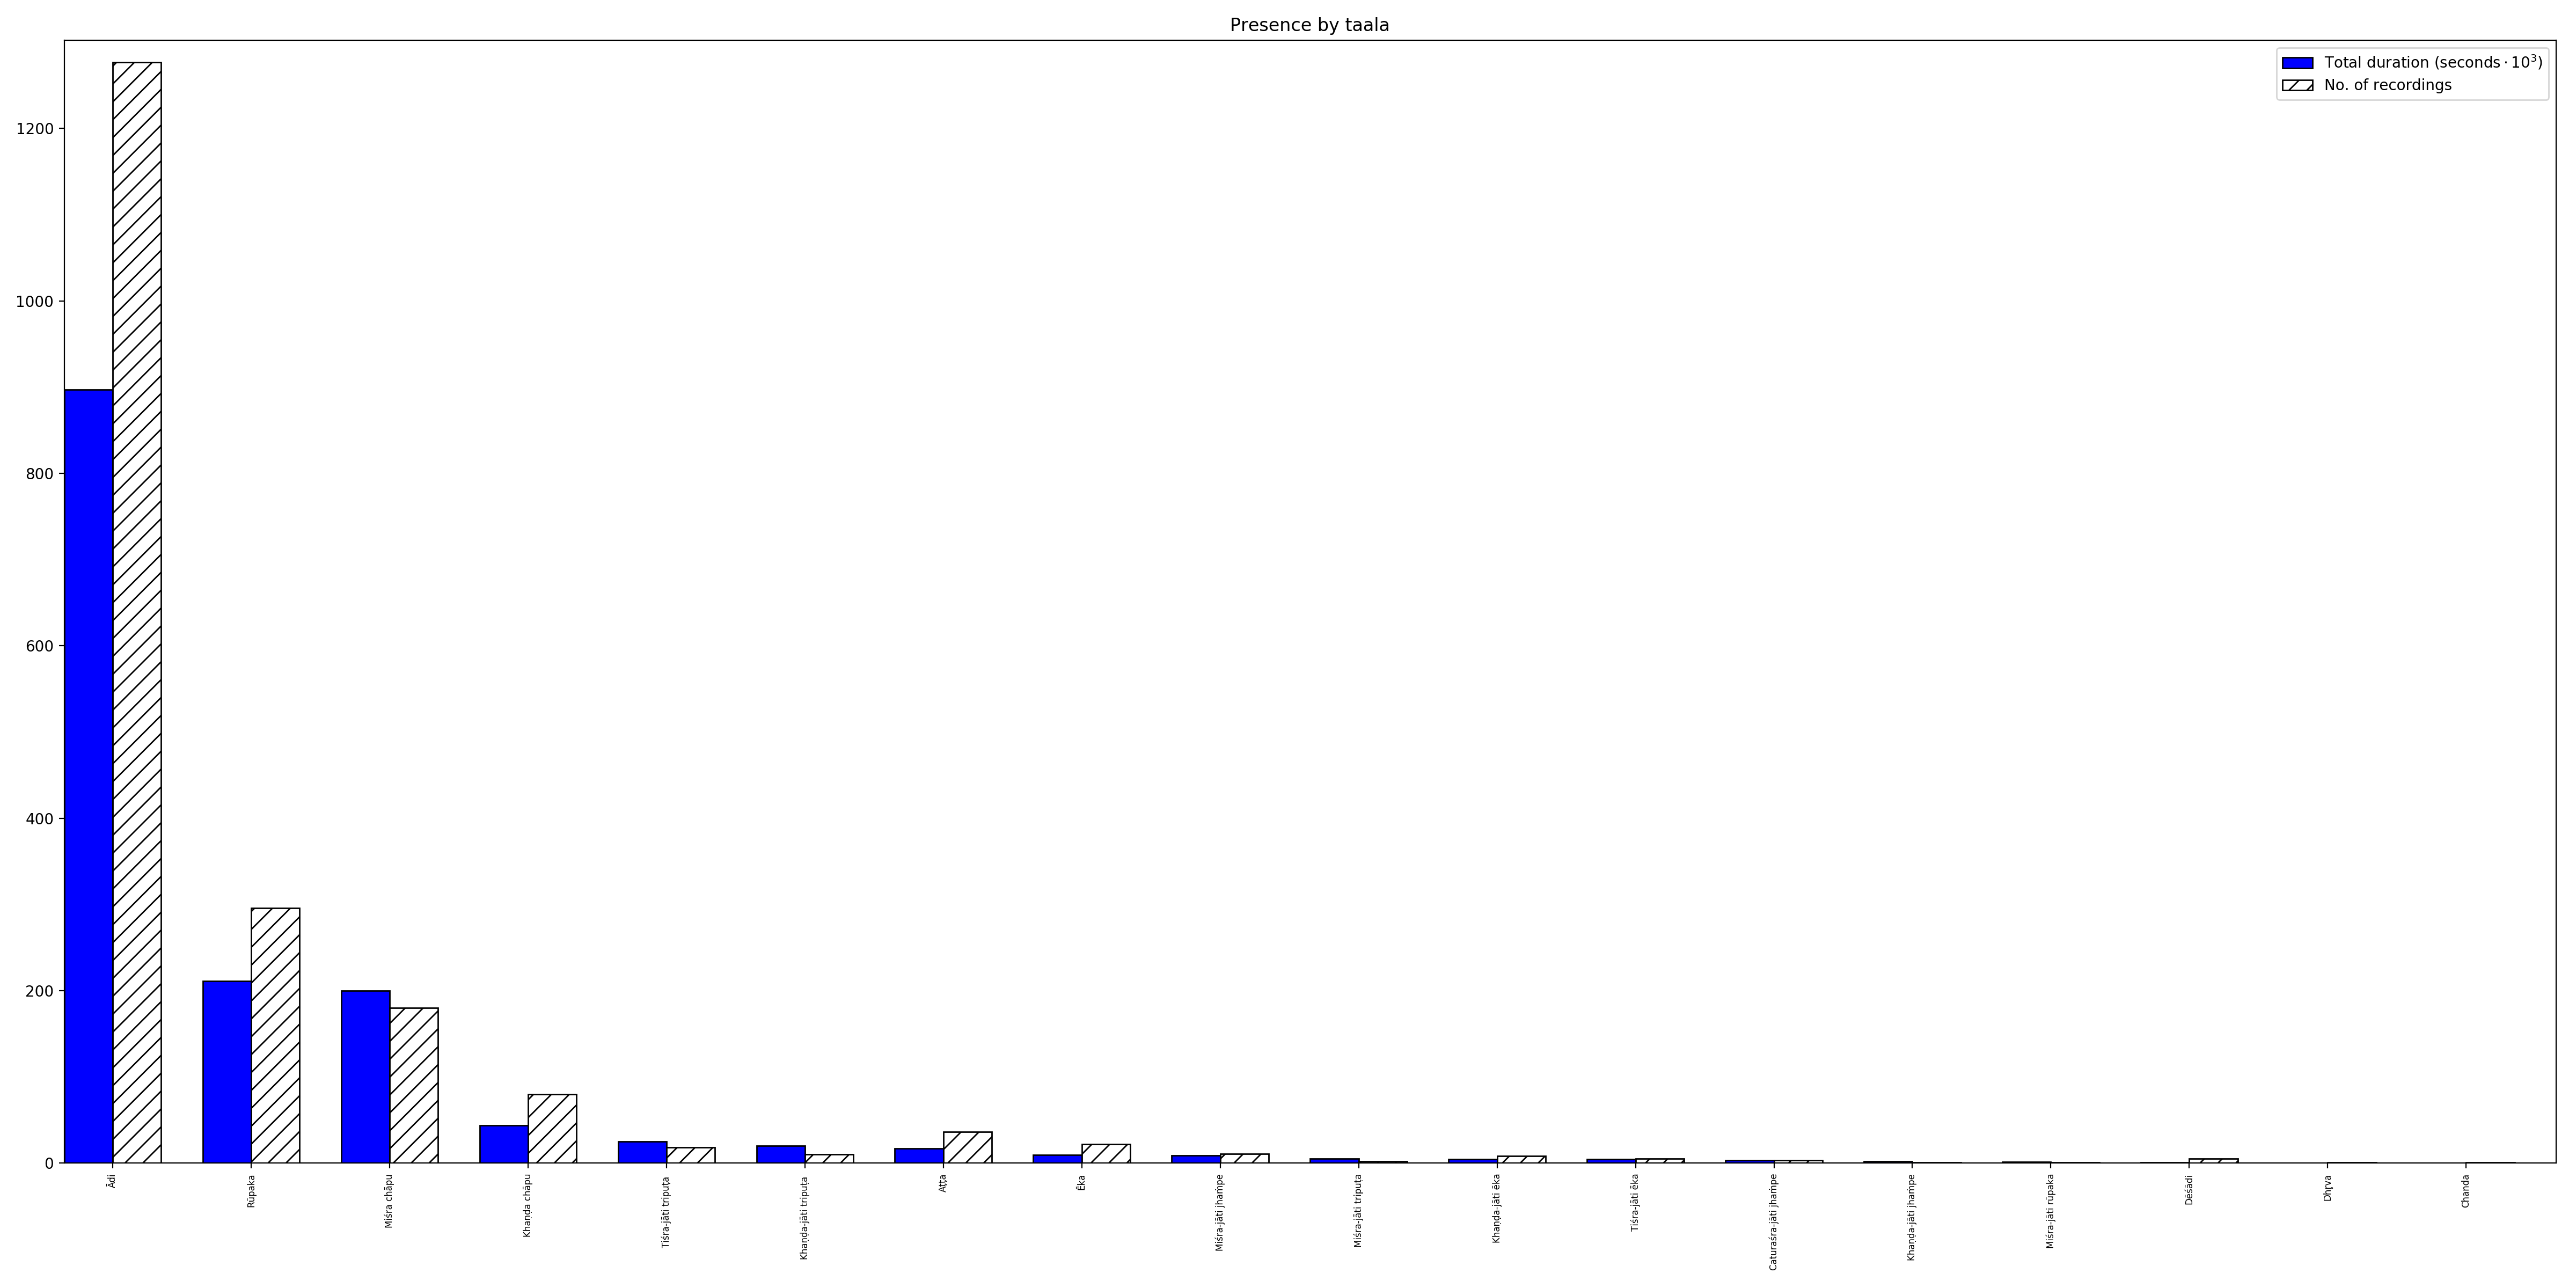
\includegraphics[scale=0.41]{histogram_taala.png}
  \caption{The number and total duration of the recordings labeled with t\=ala.}
  % \label{fig:_}
\end{sidewaysfigure}


\begin{sidewaysfigure}%[h]
  % \hspace*{-0.6cm}
  \centering
  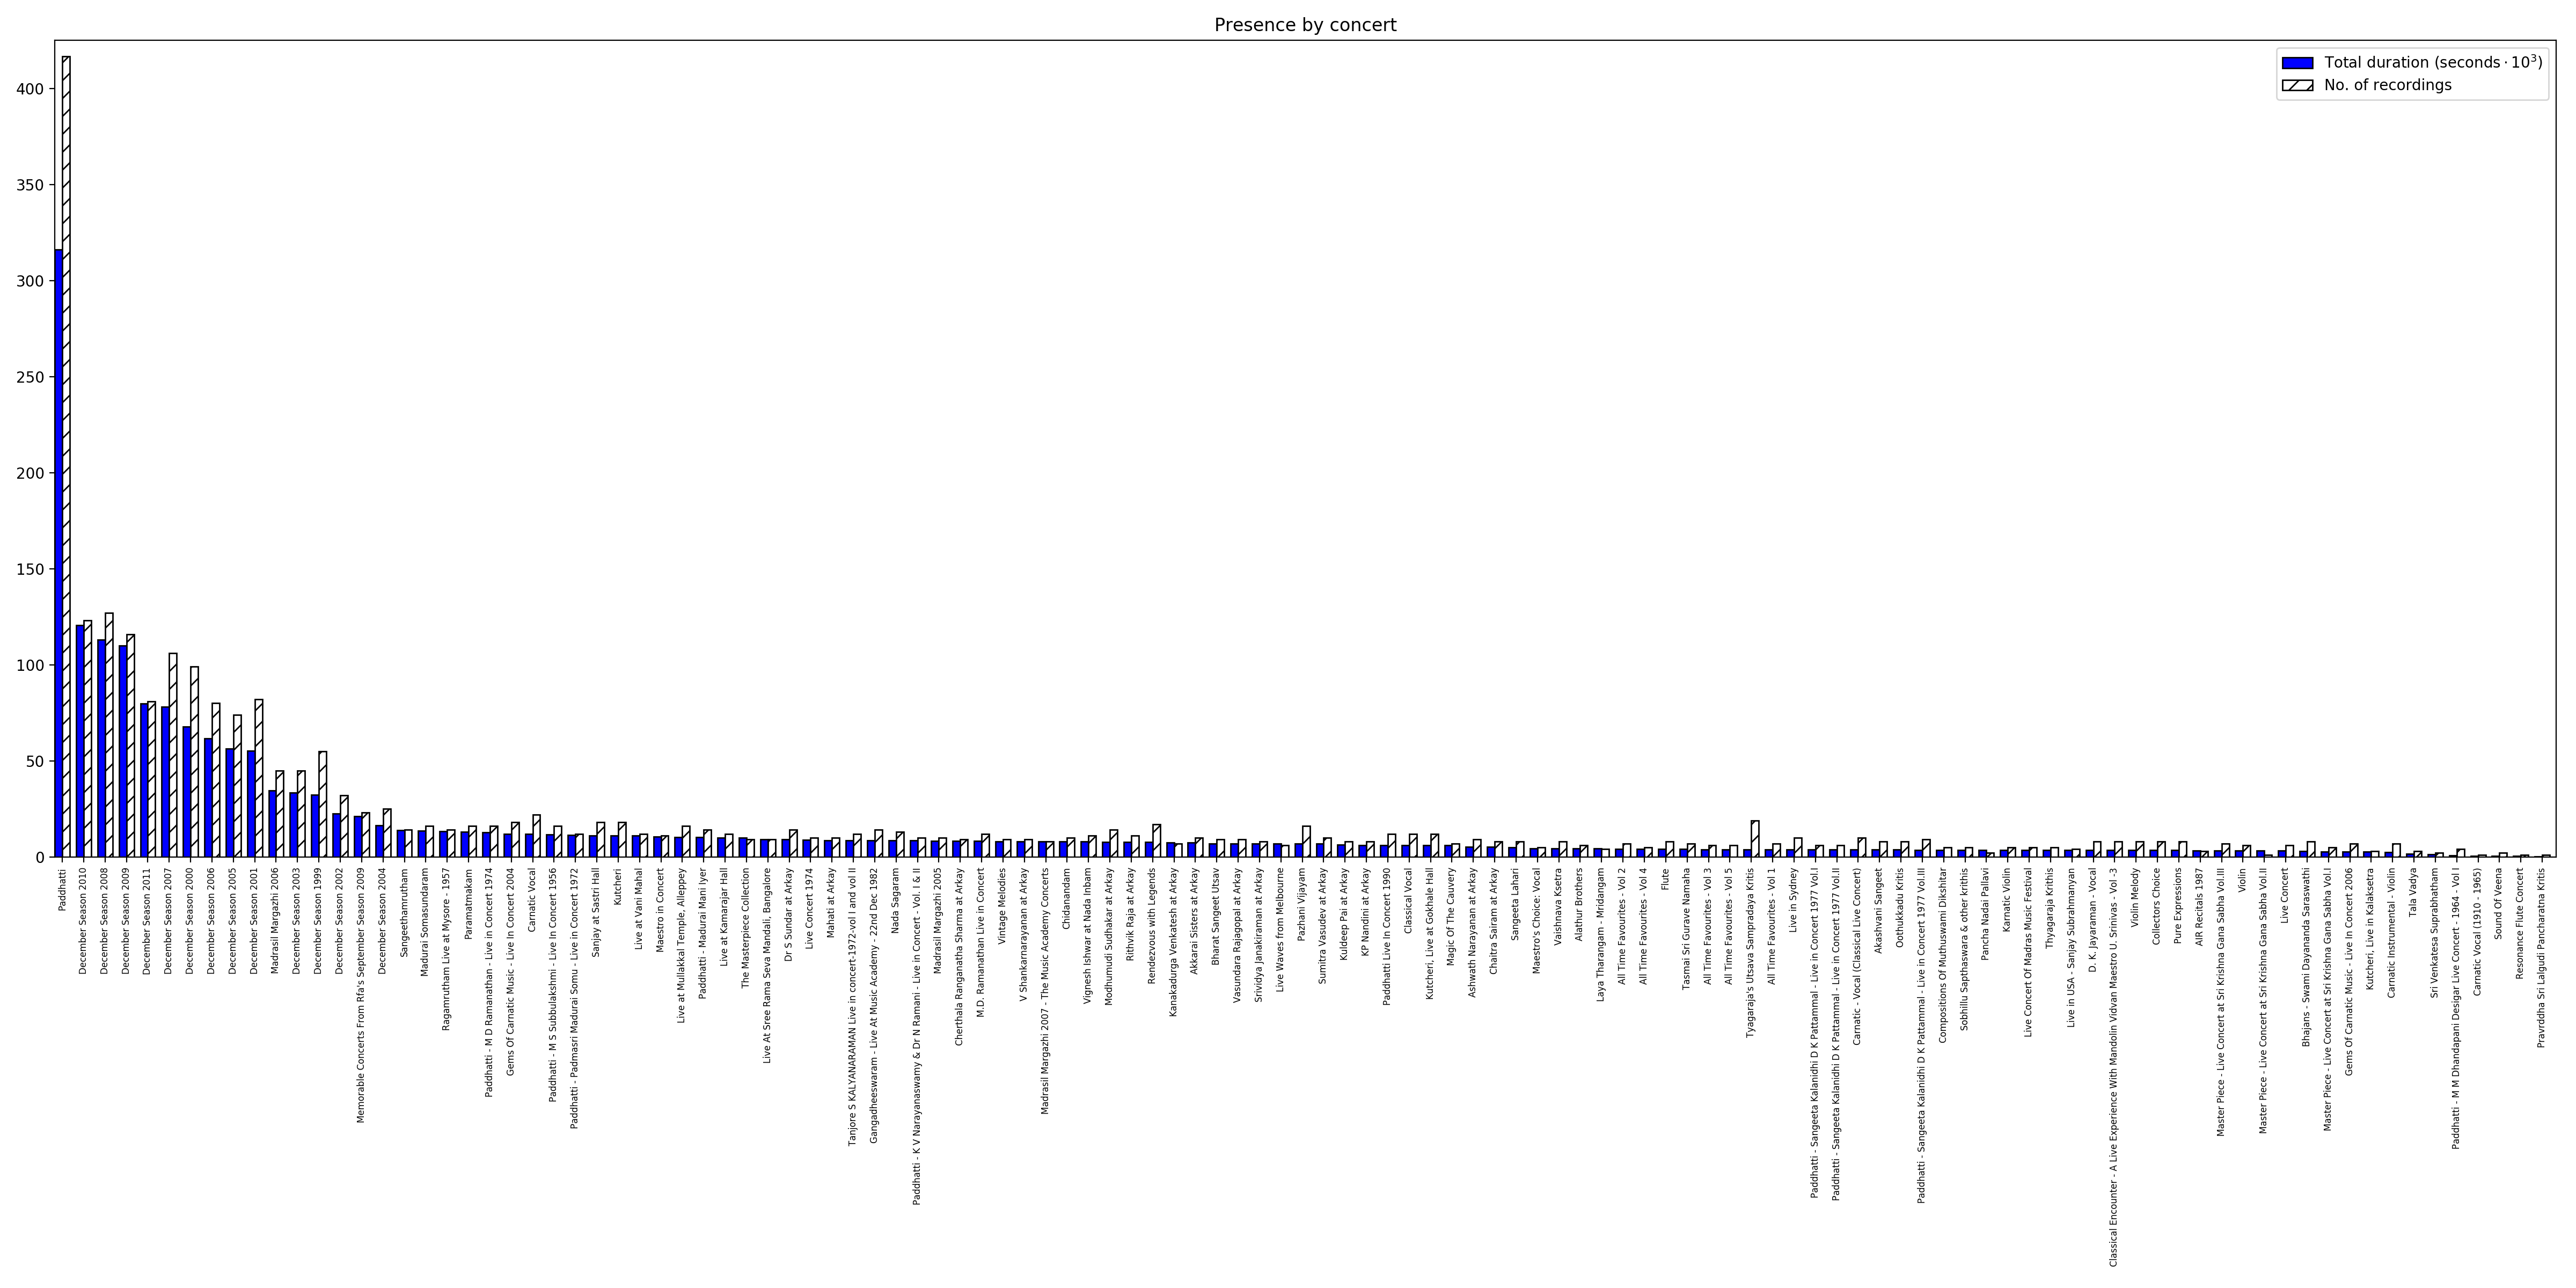
\includegraphics[scale=0.41]{histogram_concert.png}
  \caption{The number and total duration of the recordings labeled with concert.}
  % \label{fig:_}
\end{sidewaysfigure}

\begin{sidewaysfigure}%[h]
  % \hspace*{-0.6cm}
  \centering
  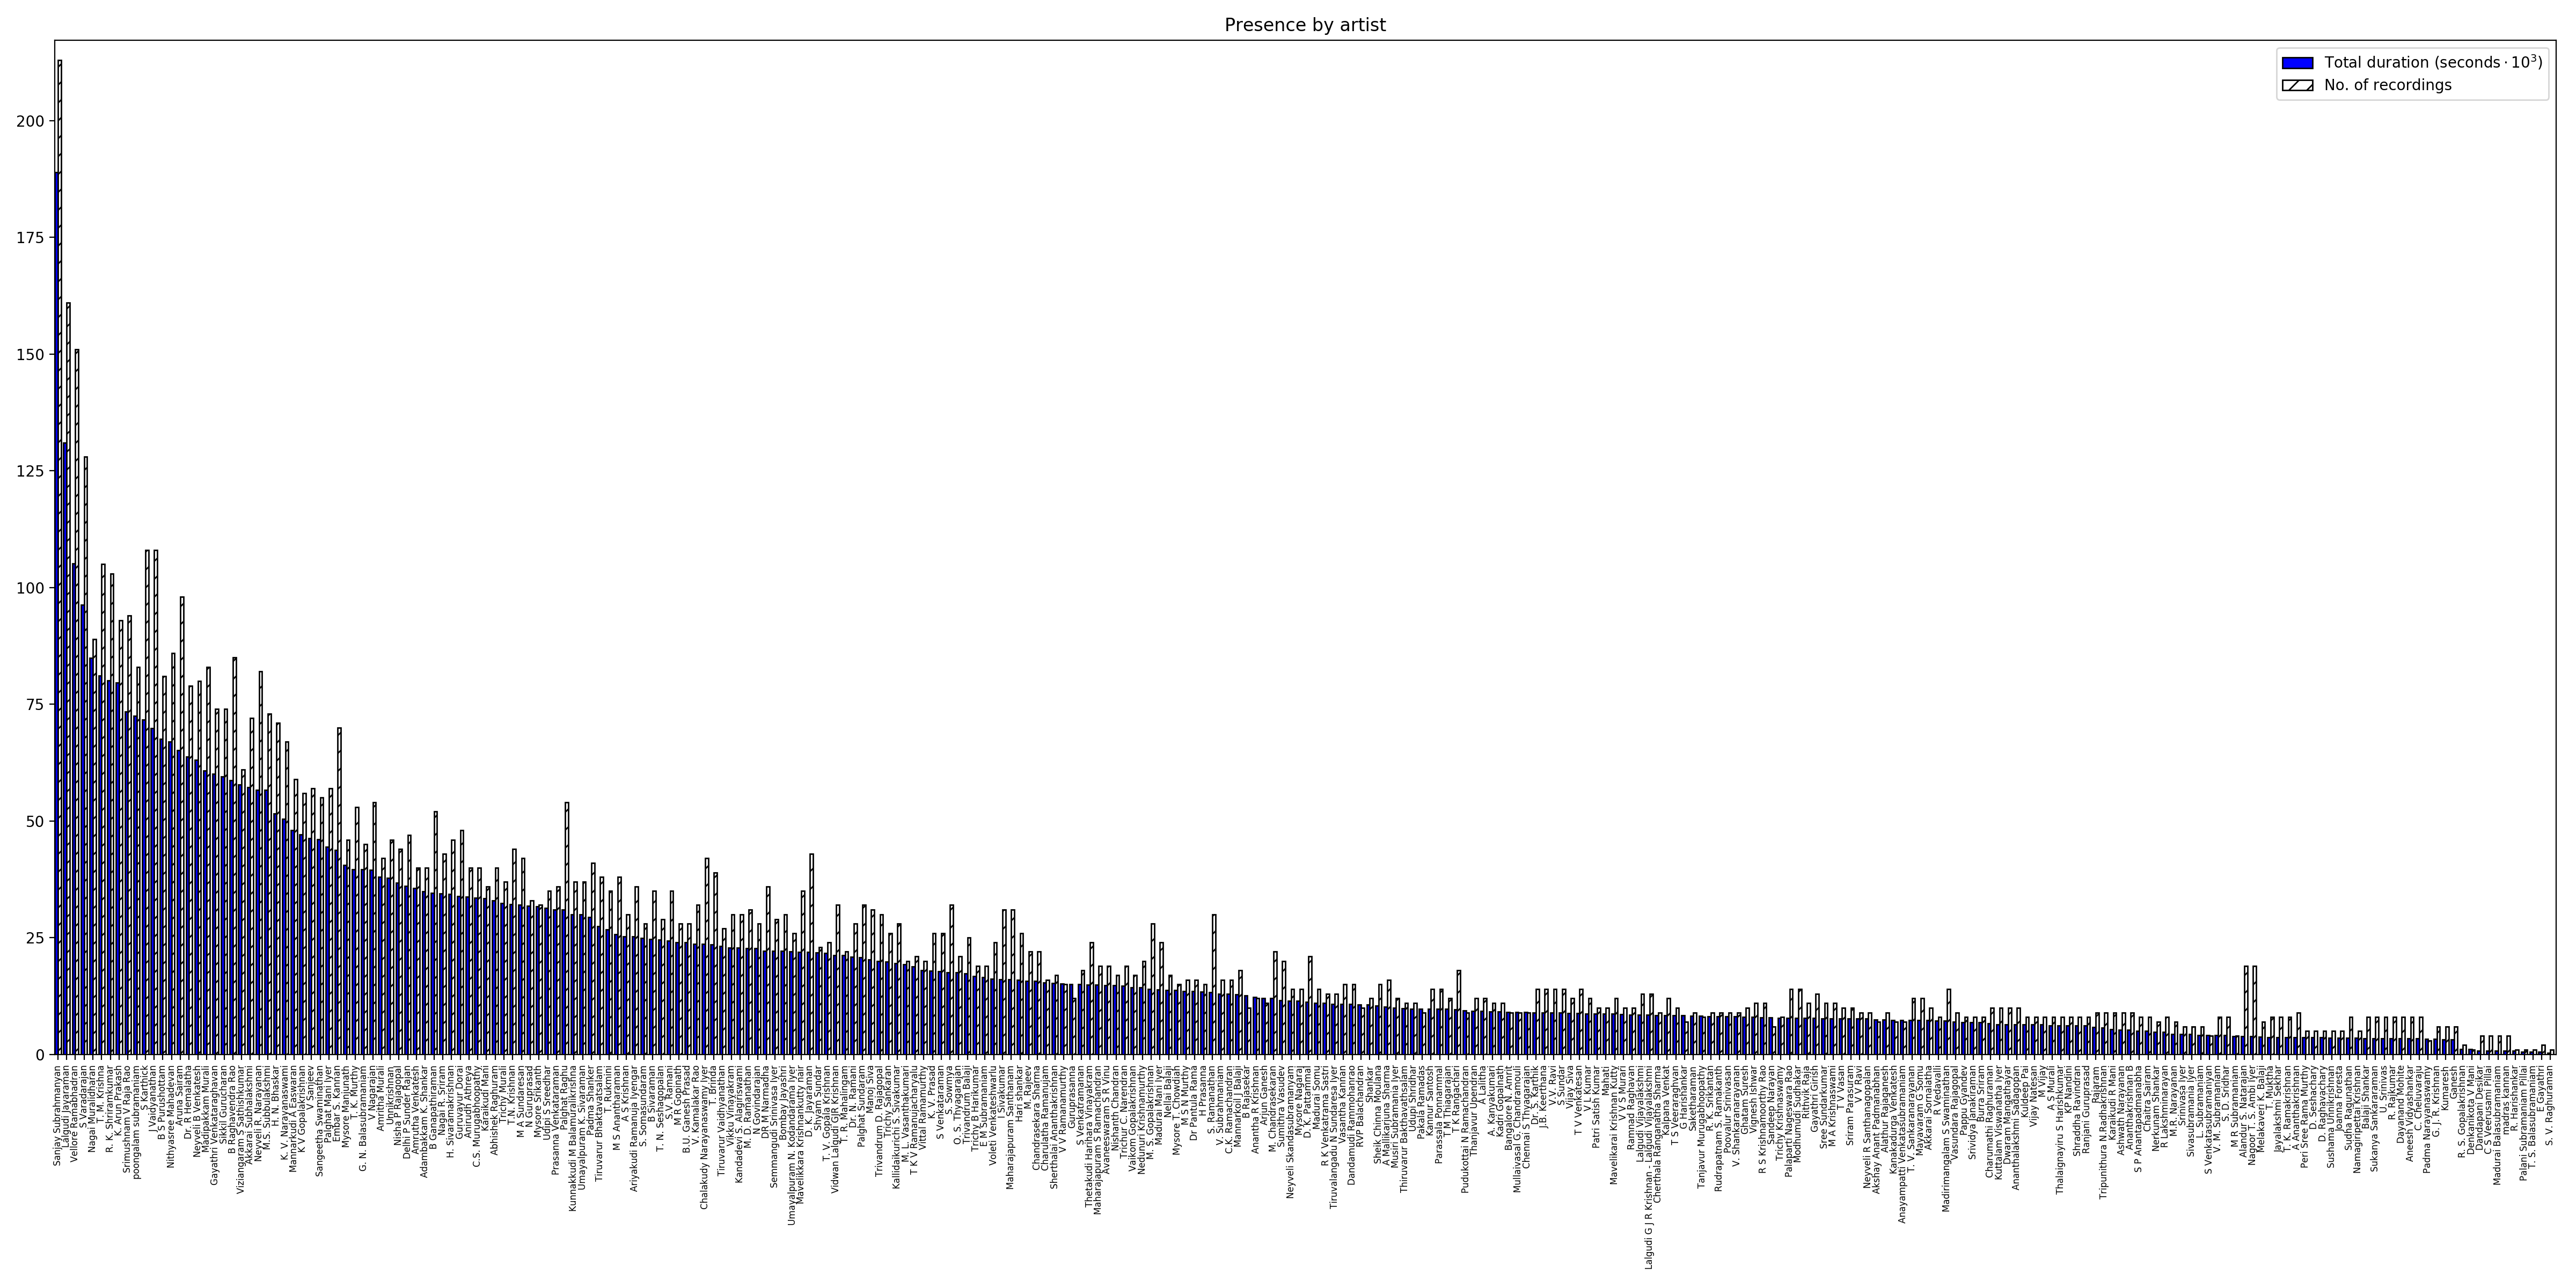
\includegraphics[scale=0.41]{histogram_artist.png}
  \caption{The number and total duration of the recordings labeled with artist.}
  % \label{fig:_}
\end{sidewaysfigure}


\begin{sidewaysfigure}%[h]
  % \hspace*{-0.6cm}
  \centering
  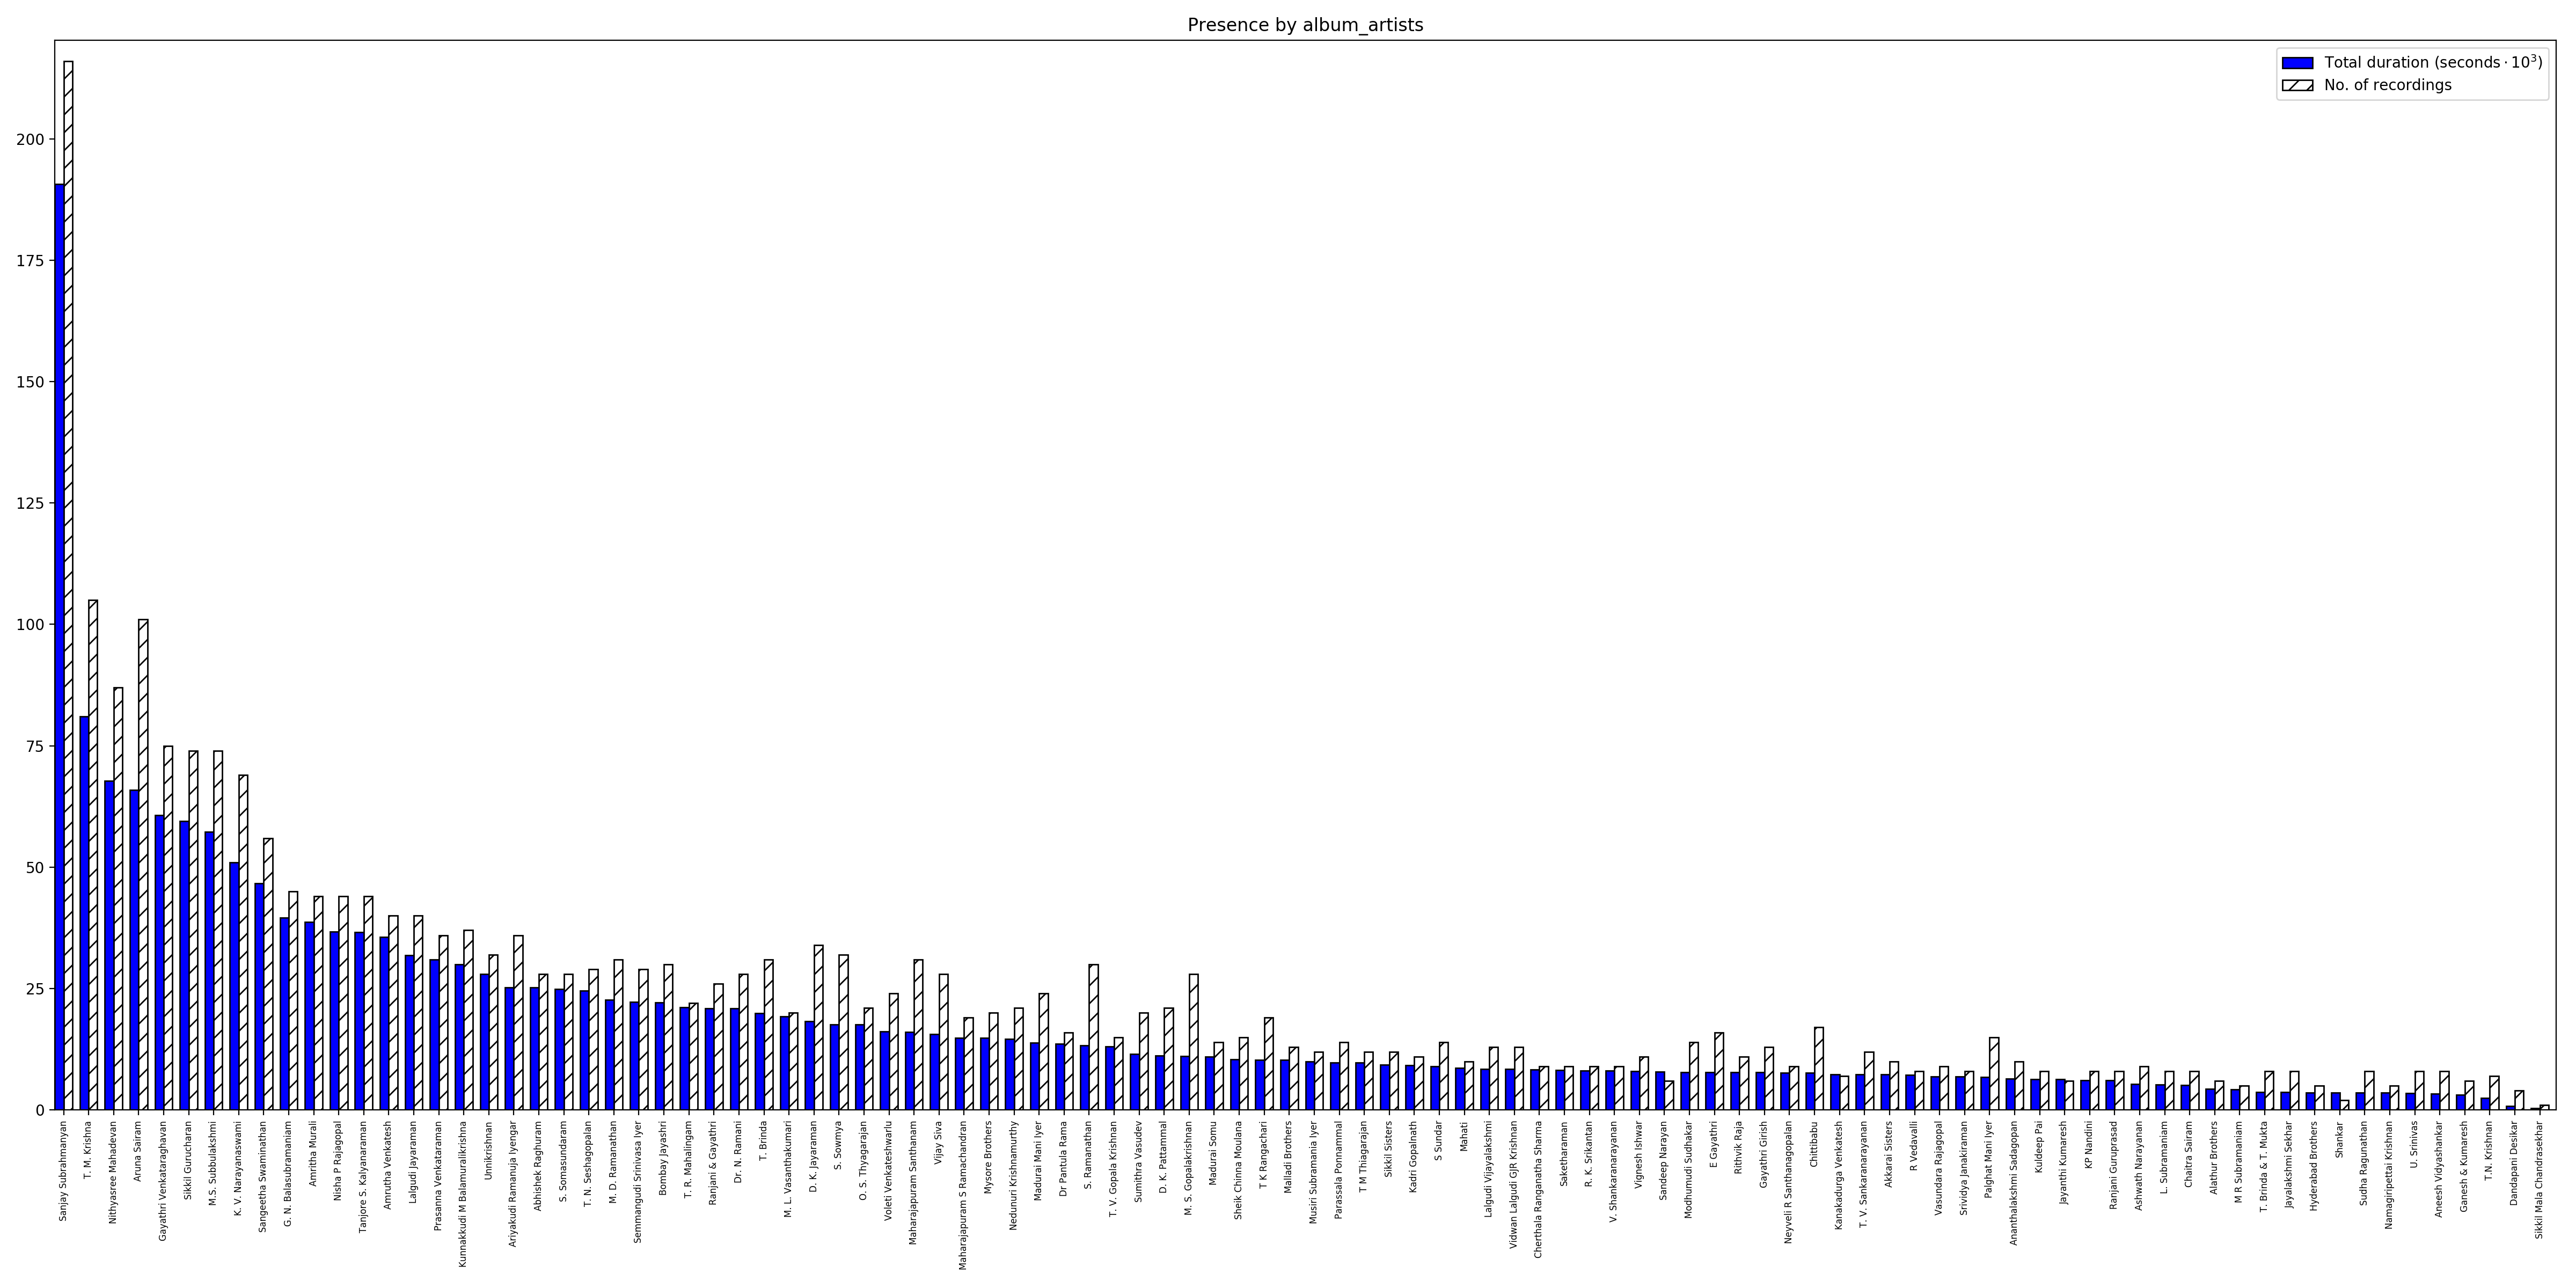
\includegraphics[scale=0.41]{histogram_album_artists.png}
  \caption{The number and total duration of the recordings labeled with album artist.}
  % \label{fig:_}
\end{sidewaysfigure}


\begin{sidewaysfigure}%[h]
  % \hspace*{-0.6cm}
  \centering
  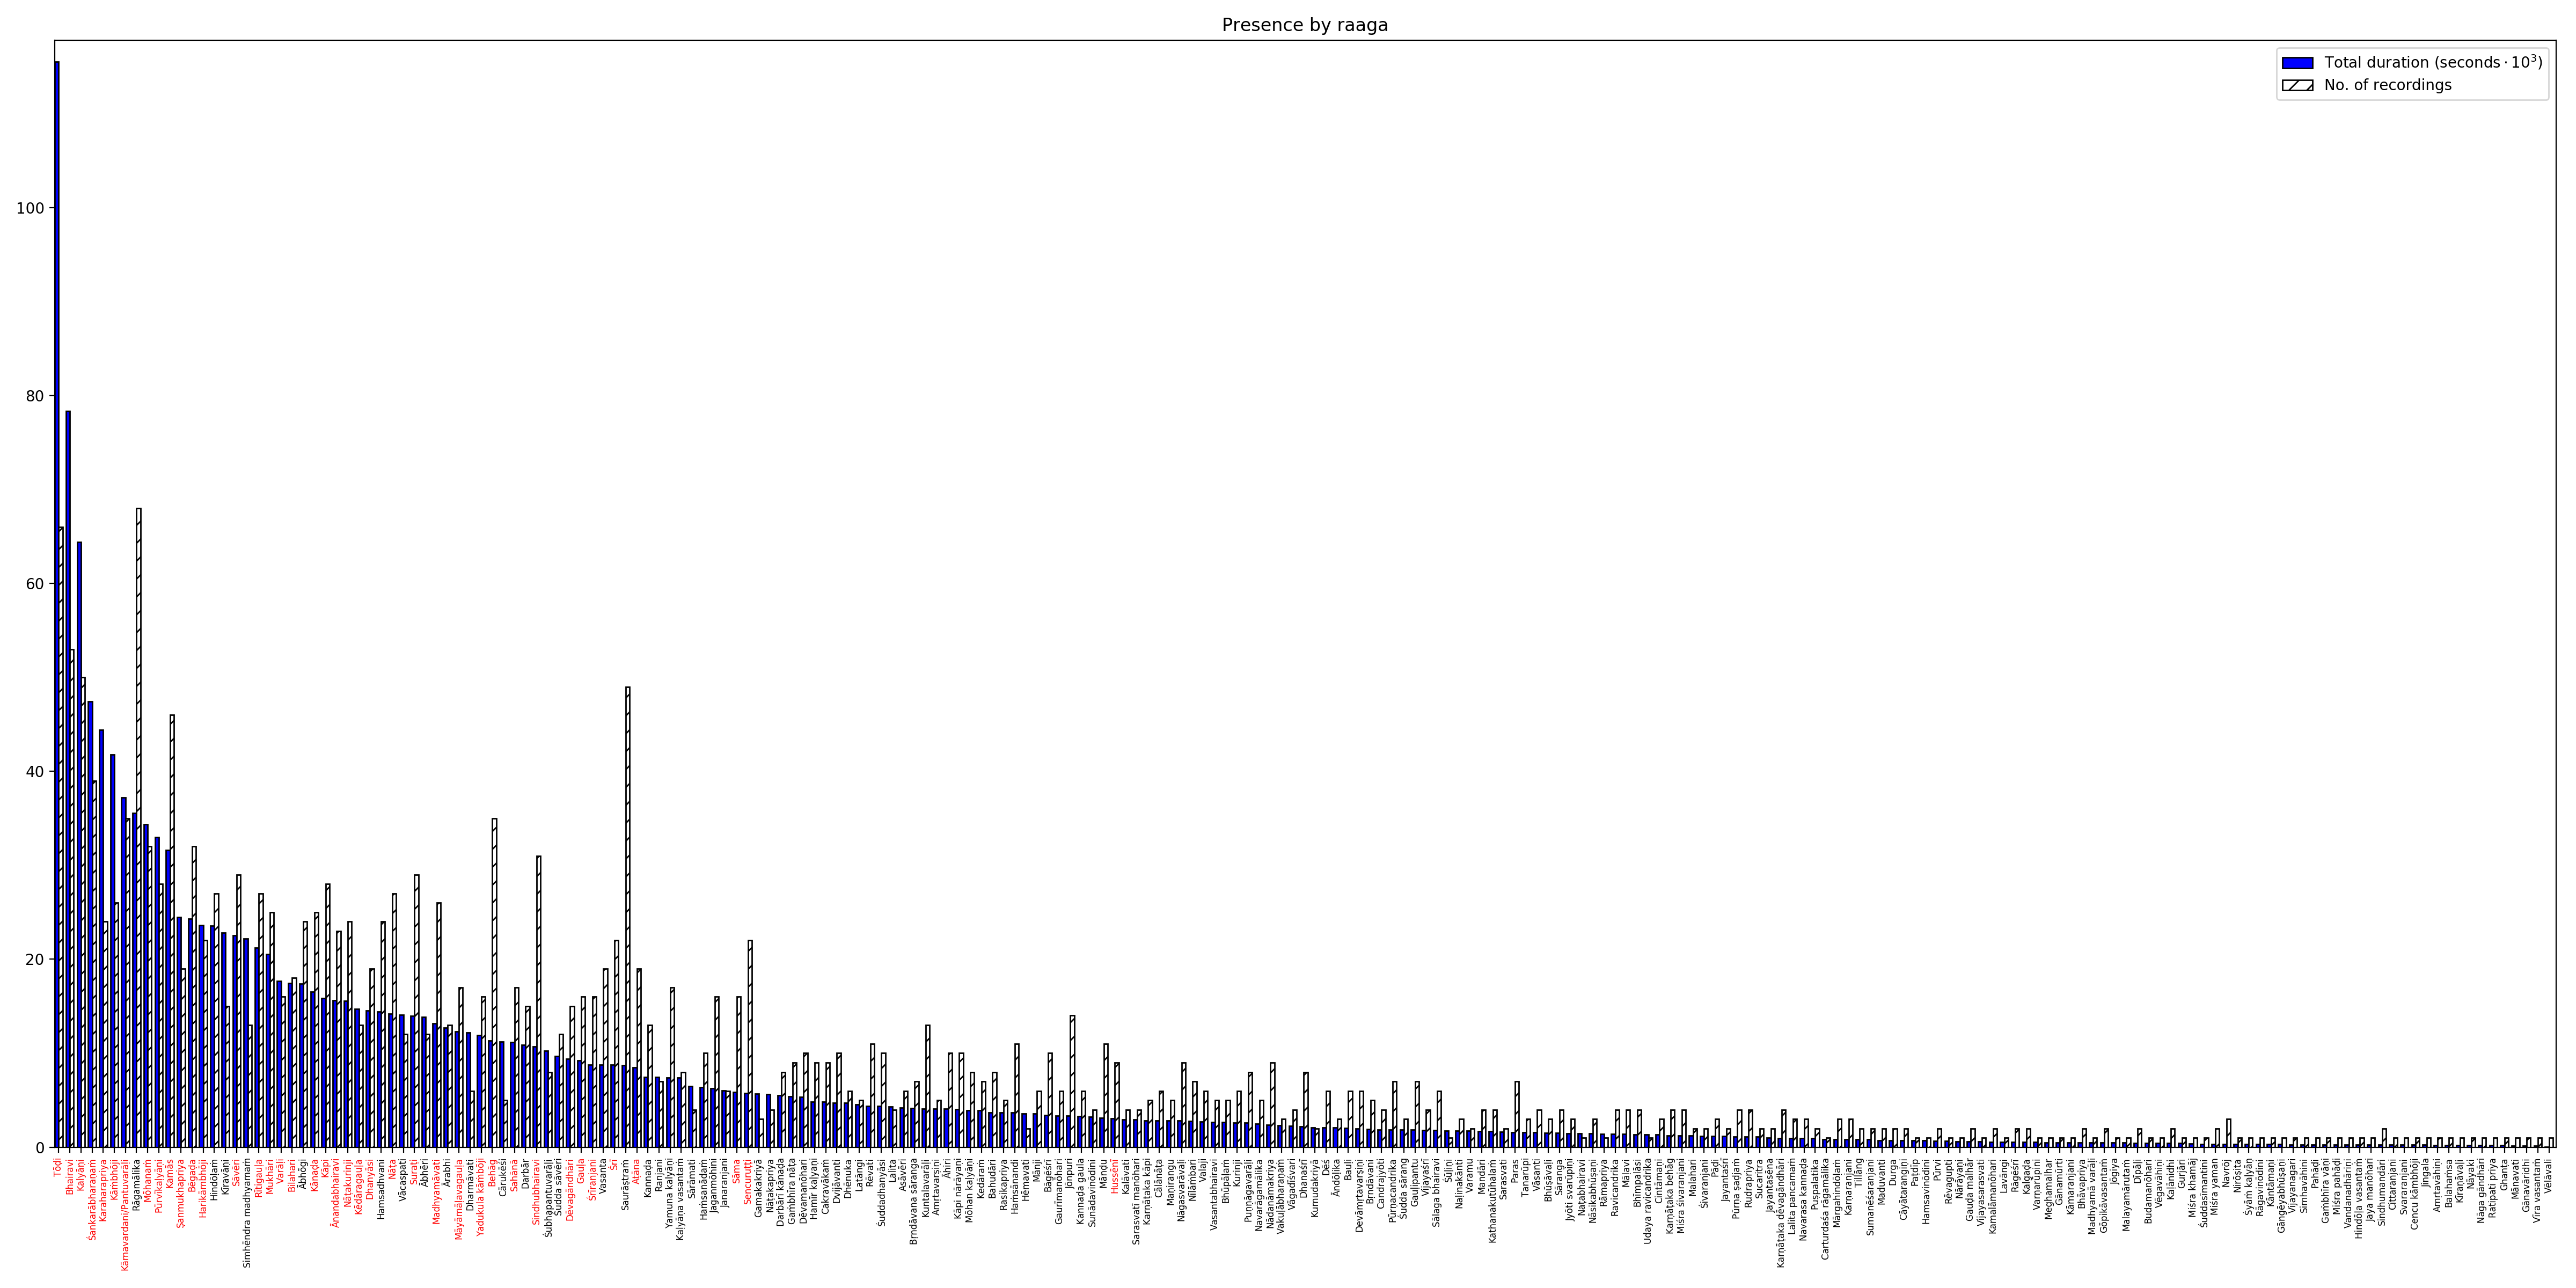
\includegraphics[scale=0.41]{histogram_raaga.png}
  \caption{The number and total duration of the recordings labeled with r\=aga. In red are the r\=agas present in Gulati's \(RRD_{CMD}\) test set.}
  % \label{fig:_}
\end{sidewaysfigure}


\begin{table}
  \centering
  \resizebox{\textwidth*7/8}{!}{%
    \begin{tabular}{*5c}\toprule
      \bfseries R\=aga & \bfseries \#Recordings & \bfseries Total duration & \bfseries Dur. in RRD_{CMD} & \bfseries Dur. in corpus\\\Midrule
      T\=o\d{d}i                       & 12 & 7h15m31s &      6.38\% &      12.15\%  \\\midrule
      Bhairavi                         & 12 & 5h18m19s &      4.66\% &      8.24\%  \\\midrule
      Kaly\=a\d{n}i                    & 11 & 5h17m19s &      4.65\% &      6.77\%  \\\midrule
      Śankar\=abhara\d{n}a\.{m}        & 10 & 3h42m47s &      3.26\% &      4.99\%  \\\midrule
      Karaharapriya                    & 11 & 6h42m03s &      5.89\% &      4.67\%  \\\midrule
      K\=a\.{m}bh\=oji                 & 10 & 5h19m24s &      4.68\% &      4.39\%  \\\midrule
      K\=amavardani                    & 12 & 3h30m49s &      3.09\% &      3.91\%  \\\midrule
      M\=ohana\.{m}                    & 12 & 4h40m04s &      4.10\% &      3.61\%  \\\midrule
      P\=urv\={\i}ka\d{l}y\=a\d{n}i    & 12 & 5h51m54s &      5.15\% &      3.47\%  \\\midrule
      Kam\=as                          & 11 & 2h13m00s &      1.95\% &      3.33\%  \\\midrule
      \d{S}anmukhapriya                & 12 & 2h59m15s &      2.63\% &      2.58\%  \\\midrule
      B\=ega\d{d}a                     & 12 & 2h51m39s &      2.51\% &      2.56\%  \\\midrule
      Harik\=ambh\=oji                 & 11 & 3h57m57s &      3.49\% &      2.49\%  \\\midrule
      S\=av\=eri                       & 10 & 2h23m58s &      2.11\% &      2.37\%  \\\midrule
      R\={\i}tigau\d{l}a               & 12 & 3h13m50s &      2.84\% &      2.23\%  \\\midrule
      Mukh\=ari                        & 12 & 3h17m55s &      2.90\% &      2.16\%  \\\midrule
      Var\=a\d{l}i                     & 9  & 2h56m58s &      2.59\% &      1.86\% \\\midrule
      Bilahari                         & 10 & 3h05m57s &      2.72\% &      1.83\%  \\\midrule
      K\=ana\d{d}a                     & 11 & 2h43m42s &      2.40\% &      1.74\%  \\\midrule
      K\=api                           & 11 & 1h05m28s &      0.96\% &      1.67\%  \\\midrule
      \=Anandabhairavi                 & 11 & 1h42m04s &      1.50\% &      1.64\%  \\\midrule
      N\=a\d{t}akurinji                & 12 & 1h45m13s &      1.54\% &      1.64\%  \\\midrule
      K\=ed\=aragau\d{l}a              & 11 & 3h58m17s &      3.49\% &      1.55\%  \\\midrule
      Dhany\=asi                       & 11 & 2h24m28s &      2.12\% &      1.53\%  \\\midrule
      N\=a\d{t}a                       & 11 & 1h37m13s &      1.42\% &      1.49\%  \\\midrule
      Sura\d{t}i                       & 12 & 2h17m57s &      2.02\% &      1.47\%  \\\midrule
      Madhyam\=avati                   & 10 & 2h15m56s &      1.99\% &      1.39\%  \\\midrule
      M\=ay\=am\=a\d{l}avagau\d{l}a    & 10 & 2h06m07s &      1.85\% &      1.30\%  \\\midrule
      Yaduku\.{l}a k\=a\.{m}b\=oji     & 10 & 1h53m48s &      1.67\% &      1.26\%  \\\midrule
      Beh\=ag                          & 12 & 1h12m59s &      1.07\% &      1.19\%  \\\midrule
      Sah\=an\=a                       & 11 & 2h30m08s &      2.20\% &      1.18\%  \\\midrule
      Sindhubhairavi                   & 12 & 1h01m05s &      0.89\% &      1.12\%  \\\midrule
      D\=evag\=andh\=ari               & 12 & 2h13m36s &      1.96\% &      0.99\%  \\\midrule
      Gau\d{l}a                        & 12 & 2h00m09s &      1.76\% &      0.97\%  \\\midrule
      Śr\={\i}ranjani                  & 9  & 1h19m32s &      1.17\% &      0.92\% \\\midrule
      Śr\={\i}                         & 9  & 0h52m09s &      0.76\% &      0.92\% \\\midrule
      A\d{t}\=ana                      & 11 & 1h35m05s &      1.39\% &      0.89\%  \\\midrule
      S\=ama                           & 10 & 0h55m48s &      0.82\% &      0.62\%  \\\midrule
      Sencuru\d{t}\d{t}i               & 12 & 0h53m35s &      0.78\% &      0.60\%  \\\midrule
      Huss\=en\={\i}                   & 8  & 0h43m18s &      0.63\% &      0.32\%  \\\bottomrule
  \end{tabular}}
  \caption{The number of recordings and total duration for each of the 40 r\=agas present in Gulati's \(RRD_{CMD}\) test set that were found in the Dunya database, as well as their relative durations with respect to the \(RRD_{CMD}\) dataset and the whole downloaded carnatic corpus.}
  \label{fig:rrd-stats}
\end{table}


\chapter{Bibliography}
\printbibliography






\end{document}
